% For printing in a4
\documentclass[a4,10pt,twoside,openright,italian,english]{book}% twoside!

% For printing with the A5 format
%\documentclass[10pt,twoside,openright,english,italian]{book}% twoside!

% Set paper size
\usepackage[twoside=true]{geometry}

%For printing with the weird format
%\geometry{
%	paperwidth=17cm,
%	paperheight=24cm,
%	margin=2cm,
%	top=2.3cm,
%	bindingoffset=0.4cm
%}
% For printing in a4
\geometry{a4paper,
  margin=3cm,
  top=3.8cm,
  bindingoffset=0.4cm
}

%Uncomment this for final prints: this just enables printing on a4 paper
\usepackage[cam,center,a4,pdflatex,axes]{crop}

\usepackage{phdthesis}

\usepackage{fancyhdr}
\usepackage{color}
\usepackage{array}
\usepackage{mdwmath}
\usepackage{mdwtab}
\usepackage{amsmath,amssymb}
\usepackage{cite}
\usepackage{graphicx}
\usepackage{listings}
\usepackage{subfig}
\usepackage{booktabs}
\usepackage{latexsym}
\usepackage{color}
\usepackage{url}
\usepackage{bnf}
\usepackage{rotating}
\usepackage{multirow}
\usepackage{phdtitle}
\usepackage{paralist}
\usepackage{xcolor}

\usepackage{bibentry}
%\usepackage[algochapter]{algorithm2e}
\usepackage[bookmarks=true,
%pdftex=false,
bookmarksopen=true,hidelinks]{hyperref}
\usepackage[toc,acronym]{glossaries}
\usepackage{lscape}
\usepackage{algorithmic}
\usepackage{algorithm}
\usepackage{longtable}
\usepackage[T1]{fontenc} 
%\usepackage[latin1]{inputenc}
\usepackage[utf8]{inputenc}
%\usepackage{fontspec}
%\setmainfont{Calibri}
%% \hyphenation{} is used to force the 
\hyphenation{}
%%%%%%%%%%%%%%%%%%%%%%%%%%%
%% For Jupyter outputs %%
%%%%%%%%%%%%%%%%%%%%%%%%%%%
%%%%%%%%%%%%%%%%%%%%%%%%%%%
%%%%%%%%%%%%%%%%%%%%%%%%%%%
%%%%%%%%%%%%%%%%%%%%%%%%%%%


\usepackage{xcolor}
\usepackage[mathletters]{ucs}
\usepackage{fancyvrb}

\newcommand{\cfr}[1]{{\textcolor{blue}[\textcolor{orange}{\bf{FR: }}{ \textcolor{blue}
              {#1}]}}}

% For linebreaks inside Verbatim environment from package fancyvrb. 
    \makeatletter
        \newbox\Wrappedcontinuationbox 
        \newbox\Wrappedvisiblespacebox 
        \newcommand*\Wrappedvisiblespace {\textcolor{red}{\textvisiblespace}} 
        \newcommand*\Wrappedcontinuationsymbol {\textcolor{red}{\llap{\tiny$\m@th\hookrightarrow$}}} 
        \newcommand*\Wrappedcontinuationindent {3ex } 
        \newcommand*\Wrappedafterbreak {\kern\Wrappedcontinuationindent\copy\Wrappedcontinuationbox} 
        % Take advantage of the already applied Pygments mark-up to insert 
        % potential linebreaks for TeX processing. 
        %        {, <, #, %, $, ' and ": go to next line. 
        %        _, }, ^, &, >, - and ~: stay at end of broken line. 
        % Use of \textquotesingle for straight quote. 
        \newcommand*\Wrappedbreaksatspecials {% 
            \def\PYGZus{\discretionary{\char`\_}{\Wrappedafterbreak}{\char`\_}}% 
            \def\PYGZob{\discretionary{}{\Wrappedafterbreak\char`\{}{\char`\{}}% 
            \def\PYGZcb{\discretionary{\char`\}}{\Wrappedafterbreak}{\char`\}}}% 
            \def\PYGZca{\discretionary{\char`\^}{\Wrappedafterbreak}{\char`\^}}% 
            \def\PYGZam{\discretionary{\char`\&}{\Wrappedafterbreak}{\char`\&}}% 
            \def\PYGZlt{\discretionary{}{\Wrappedafterbreak\char`\<}{\char`\<}}% 
            \def\PYGZgt{\discretionary{\char`\>}{\Wrappedafterbreak}{\char`\>}}% 
            \def\PYGZsh{\discretionary{}{\Wrappedafterbreak\char`\#}{\char`\#}}% 
            \def\PYGZpc{\discretionary{}{\Wrappedafterbreak\char`\%}{\char`\%}}% 
            \def\PYGZdl{\discretionary{}{\Wrappedafterbreak\char`\$}{\char`\$}}% 
            \def\PYGZhy{\discretionary{\char`\-}{\Wrappedafterbreak}{\char`\-}}% 
            \def\PYGZsq{\discretionary{}{\Wrappedafterbreak\textquotesingle}{\textquotesingle}}% 
            \def\PYGZdq{\discretionary{}{\Wrappedafterbreak\char`\"}{\char`\"}}% 
            \def\PYGZti{\discretionary{\char`\~}{\Wrappedafterbreak}{\char`\~}}% 
        } 
        % Some characters . , ; ? ! / are not pygmentized. 
        % This macro makes them "active" and they will insert potential linebreaks 
        \newcommand*\Wrappedbreaksatpunct {% 
            \lccode`\~`\.\lowercase{\def~}{\discretionary{\hbox{\char`\.}}{\Wrappedafterbreak}{\hbox{\char`\.}}}% 
            \lccode`\~`\,\lowercase{\def~}{\discretionary{\hbox{\char`\,}}{\Wrappedafterbreak}{\hbox{\char`\,}}}% 
            \lccode`\~`\;\lowercase{\def~}{\discretionary{\hbox{\char`\;}}{\Wrappedafterbreak}{\hbox{\char`\;}}}% 
            \lccode`\~`\:\lowercase{\def~}{\discretionary{\hbox{\char`\:}}{\Wrappedafterbreak}{\hbox{\char`\:}}}% 
            \lccode`\~`\?\lowercase{\def~}{\discretionary{\hbox{\char`\?}}{\Wrappedafterbreak}{\hbox{\char`\?}}}% 
            \lccode`\~`\!\lowercase{\def~}{\discretionary{\hbox{\char`\!}}{\Wrappedafterbreak}{\hbox{\char`\!}}}% 
            \lccode`\~`\/\lowercase{\def~}{\discretionary{\hbox{\char`\/}}{\Wrappedafterbreak}{\hbox{\char`\/}}}% 
            \catcode`\.\active
            \catcode`\,\active 
            \catcode`\;\active
            \catcode`\:\active
            \catcode`\?\active
            \catcode`\!\active
            \catcode`\/\active 
            \lccode`\~`\~ 	
        }
    \makeatother

    \let\OriginalVerbatim=\Verbatim
    \makeatletter
    \renewcommand{\Verbatim}[1][1]{%
        %\parskip\z@skip
        \sbox\Wrappedcontinuationbox {\Wrappedcontinuationsymbol}%
        \sbox\Wrappedvisiblespacebox {\FV@SetupFont\Wrappedvisiblespace}%
        \def\FancyVerbFormatLine ##1{\hsize\linewidth
            \vtop{\raggedright\hyphenpenalty\z@\exhyphenpenalty\z@
                \doublehyphendemerits\z@\finalhyphendemerits\z@
                \strut ##1\strut}%
        }%
        % If the linebreak is at a space, the latter will be displayed as visible
        % space at end of first line, and a continuation symbol starts next line.
        % Stretch/shrink are however usually zero for typewriter font.
        \def\FV@Space {%
            \nobreak\hskip\z@ plus\fontdimen3\font minus\fontdimen4\font
            \discretionary{\copy\Wrappedvisiblespacebox}{\Wrappedafterbreak}
            {\kern\fontdimen2\font}%
        }%
        
        % Allow breaks at special characters using \PYG... macros.
        \Wrappedbreaksatspecials
        % Breaks at punctuation characters . , ; ? ! and / need catcode=\active 	
        \OriginalVerbatim[#1,codes*=\Wrappedbreaksatpunct]%
    }
    \makeatother





%%%%%%%%%%%%%%%%%%%%%%%%%%%
%%%%%%%%%%%%%%%%%%%%%%%%%%%
%%%%%%%%%%%%%%%%%%%%%%%%%%%
%%%%%%%%%%%%%%%%%%%%%%%%%%%
%%%%%%%%%%%%%%%%%%%%%%%%%%%
%%%%%%%%%%%%%%%%%%%%%%%%%%%


\newcommand{\posit}[2]{% \deriv[<order>]{<func>}{<var>}
  Posit\ensuremath{\left<#1,#2\right>}}

%%%%%%%%%%%%%%%%%%%%%%%%%%%
%% FOR BYTEFIELD %%%%%%%%%%

\usepackage{bytefield}
\usepackage{amsmath}
\newcommand{\colorbitbox}[3]{%
\rlap{\bitbox{#2}{\color{#1}\rule{\width}{\height}}}%
\bitbox{#2}{#3}}

\definecolor{lightcyan}{rgb}{0.84,1,1}
\definecolor{lightgreen}{rgb}{0.64,1,0.71}
\definecolor{darkgreen}{rgb}{0,0.6,0}
\definecolor{lightred}{rgb}{1,0.7,0.71}
%\definecolor{lightcyan}{rgb}{0.34,1,1}
\definecolor{asparago}{rgb}{0.48,0.62,0.36}
\definecolor{lightgreen}{rgb}{0.64,0.64,0.71}
\definecolor{lightblue}{rgb}{0,0.0,0.75}
\definecolor{amber}{rgb}{0.9, 0.75, 0.0}
\definecolor{darkamber}{rgb}{0.8, 0.65, 0.0}

\definecolor{javared}{rgb}{0.6,0,0} % for strings
\definecolor{javagreen}{rgb}{0.25,0.5,0.35} % comments
\definecolor{javapurple}{rgb}{0.5,0,0.35} % keywords
\definecolor{javadocblue}{rgb}{0.25,0.35,0.75} % javadoc
\definecolor{solarized@base03}{HTML}{002B36}
\definecolor{solarized@base02}{HTML}{073642}
\definecolor{solarized@base01}{HTML}{586e75}
\definecolor{solarized@base00}{HTML}{657b83}
\definecolor{solarized@base0}{HTML}{839496}
\definecolor{solarized@base1}{HTML}{93a1a1}
\definecolor{solarized@base2}{HTML}{EEE8D5}
\definecolor{solarized@base3}{HTML}{FDF6E3}
\definecolor{solarized@yellow}{HTML}{B58900}
\definecolor{solarized@orange}{HTML}{CB4B16}
\definecolor{solarized@red}{HTML}{DC322F}
\definecolor{solarized@magenta}{HTML}{D33682}
\definecolor{solarized@violet}{HTML}{6C71C4}
\definecolor{solarized@blue}{HTML}{268BD2}
\definecolor{solarized@cyan}{HTML}{2AA198}
\definecolor{solarized@green}{HTML}{859900}

%%%%%%%%%%%%%%%%%%%%%%%%%%%%%%%%%%%%%%%%%%%%%%%%%%%%%%%%%%%%%%%%

\newtheorem{Definition}{Definition}[section]

\lstset{tabsize=2,basicstyle=\footnotesize,breaklines=true}

\usepackage[english,italian]{babel}
\usepackage{ulem}
\normalem

\hypersetup{pdftitle={Title}, pdfauthor={Federico Rossi}}

\nobibliography*

\department {Dottorato di ricerca in Ingegneria dell'Informazione}

% Please fulfil the followed fields with your data
\author{Federico Rossi} 
\title{TBD TBD TBD TBD TBD}
\tutor{}
\supervisor{M. Cococcioni, S. Saponara}
\titleimage{img/unipi.png} %please not change
\phdyear{2022}
\phdmonth{Month}
\phdcycle{XXXV}

%%%%%%%%%%%%%%%%%%%%%%%%%%%%%%%%%%%%%%
% Let's Start The Real Document
%%%%%%%%%%%%%%%%%%%%%%%%%%%%%%%%%%%%%%
\newglossaryentry{matrix_channel}
{       name={$H^*$},
        description={Conjugate operation}
}
\newglossaryentry{trasp_x}
{       name={$[ x ]^{\rm T}$},
        description={transpose operator}
}
\newglossaryentry{vec_x}
{       name={\textbf{x}},
        description={vectors are in bold}
}
\newglossaryentry{floor_funct}
{       name={$\left\lfloor x \right\rfloor$},
        description={round to the lower integer of $x$}
}

\newacronym[longplural={Frames per Second}]{fpsLabel}{FPS}{Frame per Second}
\newacronym[longplural={Signal to Noise Ratio}]{SNRLabel}{SNR}{Signal to Noise Ratio}
\makeglossaries

\begin{document}
\selectlanguage{english}

\maketitle

\pagestyle{empty}

\cleardoublepage
\newpage

%%%%%%%%%%%%%%%%%%%%%%%%%%%%%%%%%%%%%%
% Dedication - For removing dedication, please comment or delete the code inside \thispagestyle{empty}
%%%%%%%%%%%%%%%%%%%%%%%%%%%%%%%%%%%%%%
\thispagestyle{empty}

%% change numbering into Roman numbers for the introductory part
%\setcounter{page}{1}
%\pagenumbering{Roman}

%%%%%%%%%%%%%%%%%%%%%%%%%%%%%%%%%%%%%%
% Quotes - For removing quotes, please comment or delete the code inside \thispagestyle{empty}
%%%%%%%%%%%%%%%%%%%%%%%%%%%%%%%%%%%%%%
\thispagestyle{empty}
  

%% change numbering into Roman numbers for the introductory part
\setcounter{page}{1}
\pagenumbering{Roman}

%%%%%%%%%%%%%%%%%%%%%%%%%%%%%%%%%%%%%%
% Acknowledgement
%%%%%%%%%%%%%%%%%%%%%%%%%%%%%%%%%%%%%%

\pagestyle{fancy}
% change numbering into Roman numbers for the introductory part

%%%%%%%%%%%%%%%%%%%%%%%%%%%%%%%%%%%%%%
% Summary
%%%%%%%%%%%%%%%%%%%%%%%%%%%%%%%%%%%%%%
\selectlanguage{english}
\chapter*{Summary}
\lettrine{S}{ummary} goes here.

\selectlanguage{english}

%%%%%%%%%%%%%%%%%%%%%%%%%%%%%%%%%%%%%%
% Italian Summary
%%%%%%%%%%%%%%%%%%%%%%%%%%%%%%%%%%%%%%

%There must be an Italian version of the summary
\selectlanguage{italian}
\chapter*{Sommario}
\lettrine{S}{ommario} va qui.


\selectlanguage{english}

%%%%%%%%%%%%%%%%%%%%%%%%%%%%%%%%%%%%%%
% Publications
%%%%%%%%%%%%%%%%%%%%%%%%%%%%%%%%%%%%%%

%List of publications of the PhD candidate
\selectlanguage{english}
\chapter*{List of publications}

\section*{International Journals}
\begin{enumerate}
    \item[J1)] M. Cococcioni, F. Rossi, E. Ruffaldi, S. Saponara and B. Dupont de Dinechin, "Novel Arithmetics in Deep Neural Networks Signal Processing for Autonomous Driving: Challenges and Opportunities," in IEEE Signal Processing Magazine (Q1), vol. 38, no. 1, pp. 97-110, Jan. 2021, doi: \url{https://doi.org/10.1109/MSP.2020.2988436}.
    \item[J2)] M. Cococcioni, F. Rossi, E. Ruffaldi, and S. Saponara. "Fast approximations of activation functions in deep neural networks when using posit arithmetic". Sensors 2020 (Q2), 20(5), 1515; \url{https://doi.org/10.3390/s20051515}.
    \item[J3)] M. Cococcioni, F. Rossi, E. Ruffaldi, and S. Saponara. "Fast deep neural networks for image processing using posits and ARM scalable vector extension". Journal of Real-Time Image Processing (Q2) 17, 759–771 (2020). \url{https://doi.org/10.1007/s11554-020-00984-x}
    \item[J4)] M. Cococcioni, F. Rossi, E. Ruffaldi and S. Saponara. "Vectorizing posit operations on RISC-V for faster deep neural networks: experiments and comparison with ARM SVE". Neural Comput \& Applic (Q1) 33, 10575–10585 (2021). \url{https://doi.org/10.1007/s00521-021-05814-0}
    \item[J5)] M. Cococcioni, F. Rossi, E. Ruffaldi and S. Saponara, "A Lightweight Posit Processing Unit for RISC-V Processors in Deep Neural Network Applications," in IEEE Transactions on Emerging Topics in Computing (Q1), doi: \url{https://doi.org/10.1109/TETC.2021.3120538}.
  

\end{enumerate}
\section*{International Conferences/Workshops with Peer Review}

\begin{enumerate} 
    \item [C1)] M. Cococcioni, F. Rossi, E. Ruffaldi and S. Saponara (2020). "A Fast Approximation of the Hyperbolic Tangent When Using Posit Numbers and Its Application to Deep Neural Networks". In: Applications in Electronics Pervading Industry, Environment and Society. ApplePies 2019. Lecture Notes in Electrical Engineering, vol 627. Springer, Cham. \url{https://doi.org/10.1007/978-3-030-37277-4_25}
    \item [C2)] M. Cococcioni, F. Rossi, E. Ruffaldi and S. Saponara, "Novel Arithmetics to Accelerate Machine Learning Classifiers in Autonomous Driving Applications," 2019 26th IEEE International Conference on Electronics, Circuits and Systems (ICECS), 2019, pp. 779-782, doi: \url{https://doi.org/10.1109/ICECS46596.2019.8965031}.
    \item [C3)] M. Cococcioni, F. Rossi, E. Ruffaldi and S. Saponara, "A Novel Posit-based Fast Approximation of ELU Activation Function for Deep Neural Networks," 2020 IEEE International Conference on Smart Computing (SMARTCOMP), 2020, pp. 244-246, doi: \url{10.1109/SMARTCOMP50058.2020.00053}.
    \item [C4)] M. Cococcioni, F. Rossi, E. Ruffaldi, S. Saponara, "Faster deep neural network image processing by using vectorized posit operations on a RISC-V processor," Proc. SPIE 11736, Real-Time Image Processing and Deep Learning 2021, 1173604 (12 April 2021); \url{https://doi.org/10.1117/12.2586565}
    \item [C5)] M. Cococcioni, F. Rossi, E. Ruffaldi and S. Saponara (2022). "Experimental Results of Vectorized Posit-Based DNNs on a Real ARM SVE High Performance Computing Machine". In: Applications in Electronics Pervading Industry, Environment and Society. ApplePies 2021. Lecture Notes in Electrical Engineering, vol 866. Springer, Cham. \url{https://doi.org/10.1007/978-3-030-95498-7_9}
    \item[C6)] M. Cococcioni,  F. Rossi,  E. Ruffaldi,  and S. Saponara. "Small reals representations for Deep Learning at the edge: a comparison", Next Generation Arithmetic: Third International Conference, CoNGA 2022, Singapore, March 1–3, 2022, Revised Selected Papers \url{https://doi.org/10.1007/978-3-031-09779-9_8}
    \item[C7)] F. Rossi, L. Fiaschi, M. Cococcioni, S. Saponara. Design and FPGA Synthesis of BAN Processing Unit for non-Archimedean Number Crunching, International Conference on Applications in Electronics Pervading Industry, Environment and Society (APPLEPIES 2022), to appear
\end{enumerate}



\selectlanguage{english}

%%%%%%%%%%%%%%%%%%%%%%%%%%%%%%%%%%%%%%
% List of Abbreviation and Symbols
%%%%%%%%%%%%%%%%%%%%%%%%%%%%%%%%%%%%%%
%Have a look at \gls command... you can refer a term in multiple ways
\printglossary[type=\acronymtype,title=List of Abbreviations]
\let\cleardoublepage\clearpage
\printglossary[title=Notation]
\cleardoublepage
\newpage
%%%%%%%%%%%%%%%%%%%%%%%%%%%%%%%%%%%%%%
% TOC
%%%%%%%%%%%%%%%%%%%%%%%%%%%%%%%%%%%%%%
\tableofcontents
\cleardoublepage
\newpage

% Now lets go back to normal numbering
\setcounter{page}{1}
\pagenumbering{arabic}

\cleardoublepage
\chapter{Introduction}



% A TOP DOWN APPROACH 
\chapter{Real number representations: a review}

Dealing with machine learning, linear algebra applications or whichever scientific task requires the use of real numbers. Mathematically speaking, a real number $r \in \mathbb{R}$, belongs to a continuous space. In a digital domain, where quantities are \textit{discrete}, we need to fallback to a discrete space to represent such numbers.  In particular we rely on the subset of \textit{rational} numbers $\mathbb{Q} \in \mathbb{R}$.

Theoreticaly, we could represent any rational number $q \in \mathbb{Q}$ using a couple of integer numbers $n,d \in \mathbb{Z}$ such that $\frac{n}{d} = q$. Therefore, all the operations involved between such numbers would be operations between integers, that are discrete quantities.

In practice, we typically resort to a subset $\mathbb{X} \in \mathbb{Q}$, where the different format representations lie.

\begin{figure}
    \centering
    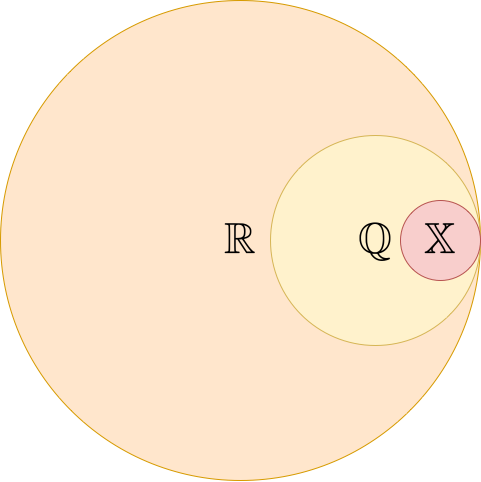
\includegraphics[width=0.3\linewidth]{img/real_sets.png}
    \caption{Visualization of real and rational number sets. $\mathbb{X}$ is the subset covered by a given format representation.}
    \label{fig:my_label}
\end{figure}

Hereafter, we will cover several real number representations, starting from the IEEE standards.


\section{The IEEE 754 Floating Point standard}

The IEEE 754 standard for floating point (\cite{893287}) defines a floating-point value as a 32,64 or 128-bit fixed-size format with three fields:
\begin{itemize}
    \item Sign (always on 1-bit) $s$
    \item Exponent $e$ (as signed integer) on $E$ bits
    \item Fractional part of the mantissa $f$ (as unsigned integer) on $F$ bits
\end{itemize}

The real value $r$ associated to a given float representation is the following:

\begin{equation}\label{eqn:float2real}
    r = (-1)^s \cdot 2^{e-k} \cdot (1.f)
\end{equation}

The expression $1.f$ is a shorthand for $1 + \frac{f}{2^F}$

The constant value $k$ is a \textit{bias} applied to the exponent for normalization purposes. The bias value is computed as follows: $k = 2^{E-1} - 1$.



\begin{table}[b]
\centering
\caption{Bit configuration for different IEEE754 floats}
\label{tab:ieee754configs}
\begin{tabular}{l|lll}
\hline
          & Exponent bits & Bias  & Fraction bits \\ \hline
Binary16 &  5             & 15    & 10            \\ \hline
Binary32  & 8             & 127   & 23            \\ \hline
Binary64  & 11            & 1023  & 52            \\ \hline
Binary128 & 15            & 16383 & 112           \\ \hline
\end{tabular}
\end{table}

The four different IEEE 754 configurations are called, respectively: binary16 (half-precision), binary32 (single-precision), binary64 (double-precision) and binary128 (quadruple-precision). Table \ref{tab:ieee754configs} summarizes the different bit configurations for the three formats.

Besides the \textit{normal} representation, there are \textit{special} bit patterns that represent special numbers:
\begin{itemize}
    \item $e = 0$ and $f \neq 0$: subnormal numbers
    \item $e = 2^{E} - 1$ and $f = 0$: infinity
    \item $e = 2^{E} - 1$ and $f \neq 0$: not a real/not a number
\end{itemize}

Subnormals are a class of numbers that fill the gap of real representations between zero and the minimum normal number. When the exponent $e$ is $0$ and the fraction is non-zero the exponent value in Equation \ref{eqn:float2real} is set to $2^{-k+1}$ and the leading $1$ in the mantissa part is removed (0.f instead of 1.f)

A particular mention goes to the representation for the real value $0$, that can be either positive or negative, having two representations.


\section{The Fixed Point representation}

Unlike floating point formats, the fixed point representation has a predefined amount of digits for the decimal part. Fixed point numbers are stored as plain integers with implicit scaling factors (e.g. the value $0.50$ can be stored as $50$ with an implicit scaling factor of 100).

Generally, a $N$-bit fixed point format has three \textit{fields}:

\begin{itemize}
    \item Sign $s$ on $1$ bit
    \item Integral part $i$ (as unsigned integer) on $I = \frac{N}{2} - 1$ bits
    \item Fractional part $f$ (as unsigned integer) on $F = \frac{N}{2}$ bit
\end{itemize}

The real value $r$ represented by a given fixed point in this format is:
\begin{equation}\label{eqn:fixed2real}
    r = (-1)^s \cdot \left( i + .f \right)
\end{equation}

Note that we can see the term $.f$ in \eqref{eqn:fixed2real} as:
\[
    \sum_k^F f_k \cdot 2^{-k} = \frac{f}{2^F}
\]

Where $f_k$ is the k-th bit of the integer $f$.

As an example we report the representation of the real number $6.25$ for a 16-bit fixed-point format.

Such format has a 7-bit integral part, that can be represented as $(6)_{10} = {(0000110)}_{2}$.
The fractional part is on 8 bits and can be represented as $ .(25)_{10} = .(0100000)_{2}$

Fixed point numbers are peculiar thanks to the fact that operations that involve such numbers can be implemented efficiently using integer arithmetic.

The algebraic sum of two fixed points can be represented as follows:
\begin{equation}\label{eqn:fixedSum}
    r_1 + r_2 = \left(i_1 \pm i_2 + \frac{f_1 \pm f_2}{2^{F}}\right)
\end{equation}

This is equivalent to sum the two fixed point representations.

Differently, the multiplication can be represented as follows:
\begin{equation}\label{eqn:fixedMul}
    r_1 \cdot r_2 = -1^{s_1 \oplus s_2}\cdot \left(i_1 * i_2 + \frac{i_1 \cdot f_2 + f_1\cdot i_2 + f_1 \cdot f_2}{2^F}\right) 
\end{equation}

As we can see this is not directly relatable to the multiplication of representations due to the cross-products between integral and fractional parts.

\section{The BFloat family: BFloat16 and BFloat8}

The Brain Float16 (BFloat16) format (\cite{burgess2019bfloat}) is a revision of the IEEE binary16 that modifies the number of allocated bits for the different fields:

\begin{itemize}
    \item Sign (always on 1-bit) $s$
    \item Exponent $e$ (as signed integer) on $8$ bits
    \item Fractional part of the mantissa $f$ (as unsigned integer) on $7$ bits
\end{itemize}

The format definition stands out for the fact that it shares the same number of bits for the exponent as binary32 does. Therefore, the exponent offset is the same, $127$ and the real value $r$ associated to a given BFloat16 is:

\begin{equation}\label{eqn:bfloat162real}
    r = (-1)^s \cdot 2^{e-127} \cdot \left(1 + \frac{f}{2^7} \right)
\end{equation}

Thanks to its similarity to the binary32 format, the BFloat16 can be seen as a truncated version of the former. This means that the conversion between the two formats is just a matter of shifting 16 positions left or right.

The Brain Float8 (BFloat8) format (\cite{naveen2019mixed}) is a further compression of the binary16 format, with the following fields:

\begin{itemize}
    \item Sign (always on 1-bit) $s$
    \item Exponent $e$ (as signed integer) on $5$ bits
    \item Fractional part of the mantissa $f$ (as unsigned integer) on $2$ bits
\end{itemize}

The format definition highlights the similarity with binary16, having the same number of exponent bits (hence, the same exponent offset). The real value $r$ associated to a given BFloat8 is:

\begin{equation}\label{eqn:bfloat82real}
    r = (-1)^s \cdot 2^{e-15} \cdot \left(1 + \frac{f}{2^2} \right)
\end{equation}

Since it shares the same number of exponent bits with binary16, the conversion between the two formats is just a matter of shifting 8 positions left or right.

The authors of \cite{naveen2019mixed} also introduced the concept of \textit{stochastic rounding}, mainly used during training of neural networks.

Suppose we want to round a floating point number $x$, with $s,e,m$ being, respectively, sign, exponent and mantissa (where $m = f/F$). The mantissa $m$ is originally represented on $k'$ bits and needs to be truncated into $\lfloor m \rfloor$ on $k$ bits. Let us define the probability: 
\begin{equation}\label{eqn:bfloat8StochProb}
    p = \frac{m - \lfloor m \rfloor}{\epsilon}
\end{equation}

where $\epsilon = 2^{-k}$.

Following the \textit{stochastic rounding approach}, the rounded value of $x$ will be:
\begin{equation}\label{eqn:bfloat8Rounded}
\text{Round}(x) = 
\left\{\begin{matrix}
s \cdot 2^e \cdot ( 1 + \lfloor m \rfloor + \epsilon) & \text{with probability } p \\ 
s \cdot 2^e \cdot ( 1 + \lfloor m \rfloor) & \text{with probability } 1-p 
\end{matrix}\right.
\end{equation}

\section{Flexpoint}
The Flexpoint format \cite{koster2017flexpoint,popescu2018flexpoint} combines fixed and floating point arithmetic. In particular, given a tensor $T$, all the values inside it are represented with a shared exponent. Each of these values is represented as a fixed-point with $N$-bits mantissa. All the values then share a common exponent on $M$ bits. The authors call such a format $\text{flex}N+M$; the counterpart for a binary32 number is $\text{flex}16+5$, according to the authors.

Thank to this approach the memory footprint of tensors are heavily reduced and, consequently, the bandwidth required by the hardware is reduced. In particular, if we employ GPU computing, we only need to transfer the integral part to the device while the shared exponent can be left on the host domain. 

The authors also propose an automatic exponent management, that adjust the exponent scale according to historical predictions of exponent changes. In particular, if the dataset contains independent and identically distributed samples, we can expect exponent values to change slowly during training epochs.

\section{Logarithmic Number System (LNS)}

The Logarithmic Number System is a system where any number $X$ is represented as follows:
\begin{equation}\label{eqn:logNumSysSet}
    X \xrightarrow[]{}\{ s,x = \log_b(\left| X \right|) \}
\end{equation}

Where $b$ is the logarithm base and $s$ the sign of the number $X$. The value $x$ is typically represented as an integer in two's complement format.

The first property that stands out from this representation is that division, multiplication and exponentiation can be transformed as follow:
\begin{equation}
    X\cdot Y \xrightarrow[]{} (s_x \oplus s_y)\cdot \left[ \log_b(X \cdot Y) \right] = (s_x \oplus s_y)\cdot \left[ \log_b(X) +  \log_b(Y) \right] = (s_x \oplus s_y)\cdot \left[ x+y \right]
\end{equation}

\begin{equation}
    \frac{X}{Y} \xrightarrow[]{} (s_x \oplus s_y)\cdot \left[ \log_b\left(\frac{X}{Y}\right) \right] = (s_x \oplus s_y)\cdot \left[ \log_b(X) -  \log_b(Y) \right] = (s_x \oplus s_y)\cdot \left[ x-y \right]
\end{equation}

\begin{equation}
    X^Y \xrightarrow[]{} \left[ \log_b(X ^ Y) \right] = (s_x \oplus s_y)\cdot \left[Y \cdot  \log_b(X)  \right] = Y\cdot x
\end{equation}

However, addition and subtraction operations are more complicated to represent. In particular, we need to employ Gaussian Logarithms:
\begin{equation}
    s_b(z) = \log_b (1 + b^z)
\end{equation}
\begin{equation}
    d_b(z) = \log_b (\left | 1 - b^z \right |)
\end{equation}

Using those two definition we can define the sum and subtraction operations as follows:
\begin{equation}
    \log_b(|X + Y|) = x + s_b(y - x) 
\end{equation}

\begin{equation}
    \log_b(|X + Y|) = x + d_b(y - x) 
\end{equation}

%\chapter{Real number representations: a review}


 % uncomment if you want part I
\chapter{Posit numbers}\label{chap:posit_num}


\lettrine{P}{osit} numbers made their first appearance in the work of John L. Gustfason "Beating Floating Point at its Own Game: Posit Arithmetic" \cite{gustafson2017beating}. The idea behind the format was to create a drop-in replacement for binary32 numbers. Posit numbers can be also seen as a new iteration of Universal Numbers (also called \textit{unum}). We can consider Posits as TypeIII unums.


Type I unums are a super-set of binary32 numbers, that is extended with an additional bit, called \textit{ubit}, that states whether the real number represented by that Unum is an exact binary32 or lies between two consecutive representations. Another difference with binary32 numbers is that unums do not have a predefined length for exponent and fraction fields. 

The second iteration of Type I unums - namely, Type II unums - points in the direction of totally abandoning the compatibility with binary32 numbers, nearing the concept of \textit{projective reals}\footnote{\url{https://en.wikipedia.org/wiki/Real_projective_line}}. The final iteration of unums is represented by the Type III Unum, also called Posit.


\section{Format and general properties}

Posit numbers are stored in two's complement integers. As shown in Figure \ref{fig:positFormat}, a Posit number is comprised of at most four fields. It can be configured on two parameters: the number of total bits \textit{nbits} and the maximum number of exponent bits \textit{esbits}
\begin{itemize}
    \item  \textcolor{asparago}{S} is the sign bit as commonly used in IEEE binary formats.
    \item \textcolor{amber}{Regime} is the regime field, on variable length; it can take up to the entire bit-space of the format after the sign bit.
    \item \textcolor{lightred}{Exponent} is the exponent field, without any bias offset; depending on $esbits$ and regime length it can span from $0$ to $esbits$ bits.
    \item \textcolor{lightgreen}{Fraction} is the fractional part of the mantissa; depending on the other fields it can be absent.
\end{itemize}


Sign, exponent and fraction have the same identical meaning as the homonymous fields in IEEE binary numbers. 

The regime field is instead new and different: its length depends on the value of the bits. In particular, the regime length depends on the number of subsequent identical bits that we find after the sign until a bit of opposite value is found. This means that, if we have this bit-string:
\begin{equation}
    b_1, b_2, b_3 \dots b_l, \overline{b_{l}}
\end{equation}
 where $b_1 = b_2 = \dots = b_l = b$, the regime length will be $l$. Depending on the value of $b$ the regime value $k$ will be computed as follows:
 
\begin{equation}\label{eqn:regimeValue}
k = \left\{\begin{matrix}
 l-1& b = 1  \\
 -l & b = 0  \\
\end{matrix}\right.
\end{equation}

The regime value is a scale factor for a special constant, that depends on the posit configuration, called \textit{useed}. The \textit{useed} value is computed as follows:
\begin{equation}\label{eqn:useed}
    \text{useed} = 2^{2^{esbits}}
\end{equation}

Wrapping everything up, the real value associated with a posit $p$ represented by the integer $P$ on two's complement (with sign $s$) is computed as in Equation \eqref{eqn:positRealValue}. The value $F$ is the length of the fraction field. Note that there will be always an implicit $1.$ in front of the fraction (i.e. $1.f_1,f_2, \dots, f_F$), without any subnormal number differently from IEEE binary numbers.

\begin{equation}\label{eqn:positRealValue}
 r =   \left\{\begin{matrix}
0 & P = 0  \\
\pm \infty & P = -2^{nbits-1}  \\
(-1)^s \cdot \text{useed}^{k} \cdot 2^e \cdot \left ( 1+ \frac{f}{2^F} \right) &  \text{otherwise} \\
\end{matrix}\right.
\end{equation}


Having the exponent and the fraction bits depending on the length of the regime is a clever way to express the so-called \textit{tapered accuracy}: numbers near $1$ (in magnitude) will have more bits allocated for the fractional part than extremely large (or small) numbers farther from $1$, thus having higher decimal accuracy. Although it highly depends on the application, the probability of encountering such extremely large or small numbers is far smaller than the one for numbers near to 1. This theoretically gives a substantial boost to posit accuracy in computations.

Figures \ref{fig:positCloseToOne} and \ref{fig:positFarFromOne} show this concept with an example. The real value $1.125$ is closer to $1$ than the value $32704$: as we can see, the number of fraction bits in the former is far greater than the one on the latter. This also reflects on the \textit{denominator} of the fraction, being $2048$ in the case of the real value $1.125$ and a quarter of that i.e. $256$ for the real value $32704$.

\begin{figure}[t]
	\centering    
    \begin{bytefield}[bitwidth=1em]{32}
       \colorbitbox{asparago}{1}{{\scriptsize{S}}}&
       \colorbitbox{amber}{10}{\scriptsize{Regime(1..$rebits$)}} &
       \colorbitbox{lightred}{9}{\scriptsize{Exponent (0..$esbits$)}} &
       \colorbitbox{lightgreen}{12}{\scriptsize{Fraction (0...)}} 
    \end{bytefield}
    \caption{The posit format}
	\label{fig:positFormat}
\end{figure}


\begin{figure}\centering\begin{bytefield}[bitwidth=0.66em]{16}\bitbox{16}{0\,1\,0\,0\,0\,0\,0\,1\,0\,0\,0\,0\,0\,0\,0\,0}\\\\\bitheader[endianness=big]{0-15}\\\colorbitbox{lightcyan}{1}{{S}}&\colorbitbox{lightgreen}{2}{R}&\colorbitbox{lightred}{2}{E}\colorbitbox{amber}{11}{F}\\\bitbox{1}{\color{cyan}0}&\bitbox{2}{\color{amber}1\!\;\color{darkamber}0}&\bitbox{2}{\color{lightred}0\!\;0}&\bitbox{11}{\color{darkgreen}0\!\;0\!\;1\!\;0\!\;0\!\;0\!\;0\!\;0\!\;0\!\;0\!\;0}&\end{bytefield}\caption{An example of Posit configuration with 16 bits and 2 exponent bits. The associated real value to the shown Posit is:$\textcolor{cyan}{1}\cdot 16^{\textcolor{darkamber}{0}}\cdot 2^{\textcolor{lightred}{0}}\cdot ( 1 + \textcolor{darkgreen}{256}/2048)= 1.125$}\label{fig:positCloseToOne}\end{figure}

\begin{figure}\centering\begin{bytefield}[bitwidth=0.66em]{16}\bitbox{16}{0\,1\,1\,1\,1\,0\,1\,0\,1\,1\,1\,1\,1\,1\,1\,1}\\\\\bitheader[endianness=big]{0-15}\\\colorbitbox{lightcyan}{1}{{S}}&\colorbitbox{lightgreen}{5}{R}&\colorbitbox{lightred}{2}{E}\colorbitbox{amber}{8}{F}\\\bitbox{1}{\color{cyan}0}&\bitbox{5}{\color{amber}1\!\;1\!\;1\!\;1\!\;\color{darkamber}0}&\bitbox{2}{\color{lightred}1\!\;0}&\bitbox{8}{\color{darkgreen}1\!\;1\!\;1\!\;1\!\;1\!\;1\!\;1\!\;1}&\end{bytefield}\caption{An example of Posit configuration with 16 bits and 2 exponent bits. The associated real value to the shown Posit is:$\textcolor{cyan}{1}\cdot 16^{\textcolor{darkamber}{3}}\cdot 2^{\textcolor{lightred}{2}}\cdot ( 1 + \textcolor{darkgreen}{255}/256)= 32704.0$}\label{fig:positFarFromOne}\end{figure}

Differently from binary32 numbers, the posit format does not have subnormal numbers. Indeed, the mantissa always has an implicit 1 and all numbers are considered in the same way. Furthermore, again in contrast with binary32 numbers, there is only one representation for infinite values or Not a Real (NaR) values. This particular bit string is represented by the integer $i = 2^{nbits - 1}$.

Given a \posit{nbits}{esbits} we can identify some important values that characterize the behaviour of the format, starting from the \textit{useed} value seen in \eqref{eqn:useed}:
\[
\text{maxposit} = useed^{(nbits - 2)}
\]

\[
\text{minposit} = \frac{1}{maxposit}
\]

As explained at the beginning of this chapter, posit numbers can be projected on a circle, called \textit{posit ring}.

\begin{figure}
\centering
\begin{minipage}{.5\textwidth}
  \centering
  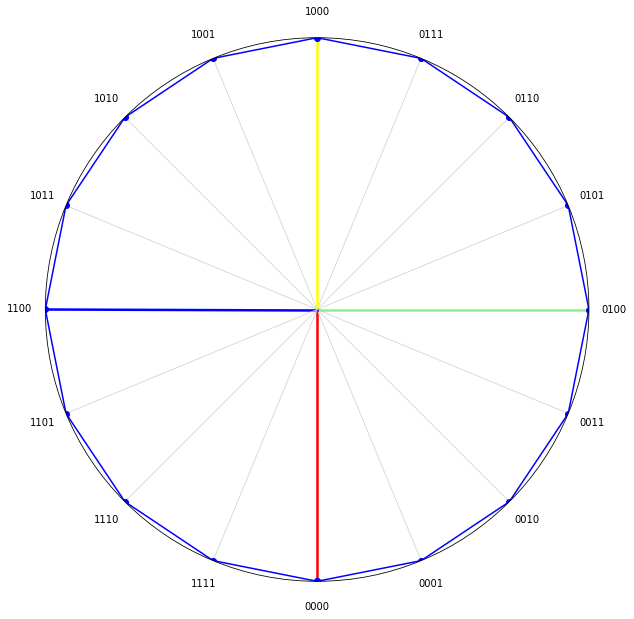
\includegraphics[width=0.9\linewidth]{img/posit4xRing.png}
  \captionof{figure}{Projection of a \posit{4}{x}}
  \label{fig:posit4xRing}
\end{minipage}%
\begin{minipage}{.5\textwidth}
  \centering
  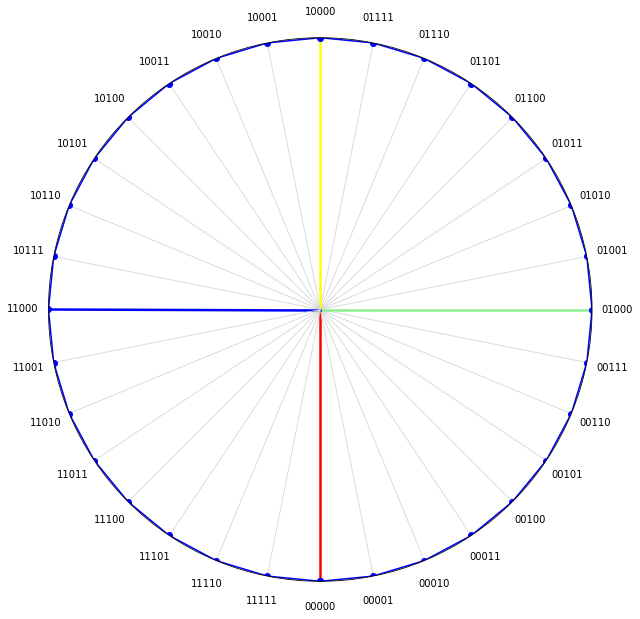
\includegraphics[width=0.9\linewidth]{img/posit5ring.png}
  \captionof{figure}{Projection of a \posit{5}{x}}
  \label{fig:posit5xRing}
\end{minipage}
\end{figure}

Figures \ref{fig:posit4xRing} and \ref{fig:posit5xRing} show the ring plot for a \posit{4}{x} and a \posit{5}{x} (exponent size is not relevant for the shape of the ring plot). The axis highlighted in \textbf{\textcolor{red}{red}} represents the real value $0$. The axis highlighted in \textbf{\textcolor{lightgreen}{green}} represents the real value $1$ and closes the first quarter of posit representations. The axis highlighted in \textbf{\textcolor{yellow}{yellow}} represents $\pm \infty$ (or \texttt{NaR}, depending on the configuration); this axis closes the quadrant where real values represented by posits are positive (note that also the integer representing the posit is positive). The axis highlighted in \textbf{\textcolor{blue}{blue}} represents the value $-1$. Note that these 4 points are fixed at south, west, north and east for any posit configuration. Indeed, they corresponds to the following posit integer representations: \textcolor{red}{0}, \textcolor{lightgreen}{$2^{nbits-2}$}, \textcolor{yellow}{$2^{nbits - 1}$} and \textcolor{blue}{$3 \cdot 2^{nbits-2}$}.

According to these two values, we can explicate the rounding, overflow and underflow behaviour of the format:
\begin{itemize}
    \item If we are trying to represent a real value $0 < r < \text{minposit}$ we will saturate it to $minposit$ to avoid underflow to $0$.
    \item If we are trying to represent a real value $r > \text{maxposit} $ we will saturate it to $\text{maxposit}$.
    \item If we are trying to represent a real value that lies between two exact posits, we need to round it to the nearest value (in terms of L2 distance).
\end{itemize}




\section{A focus on decimal accuracy}

As we said in the previous Section, since the posit format has a variable length field for the fraction, the decimal accuracy (i.e. the number of allocated fraction bits for a given number) varies across the posit domain.

In particular, the fraction field depends on the length of the regime and exponent fields; given a \posit{nbits}{esbits} the regime field can have a length 
\[
l_r \in [2,\text{nbits}-2]
\]
Consequently, the exponent field can have a length 
\[
l_e = \text{min}(\text{esbits},\text{nbits}-1-l_r)
\]

Finally, the fraction field can have a length:
\begin{equation}\label{eqn:fracFieldLength}
l_f = \text{nbits} - 1 - l_r - l_e
\end{equation}

Looking at the fraction field length in \eqref{eqn:fracFieldLength}, we see that, when the regime value $k$ (see \eqref{eqn:regimeValue}) increases in absolute value, the fraction field length decreases; this means that, when numbers are very large or very small (in absolute value) - i.e. numbers with large positive or negative regime values - the fraction field has fewer bits available for allocation. On the other hand, when the regime value decreases (in absolute value), the fraction field length increase; this means that, when numbers are very close to $1$ (in absolute value), the fraction field has more bits available for allocation. 

Having more bits available for the fraction means that we can represent more precisely numbers after the decimal dot.

\begin{figure}
    \centering
    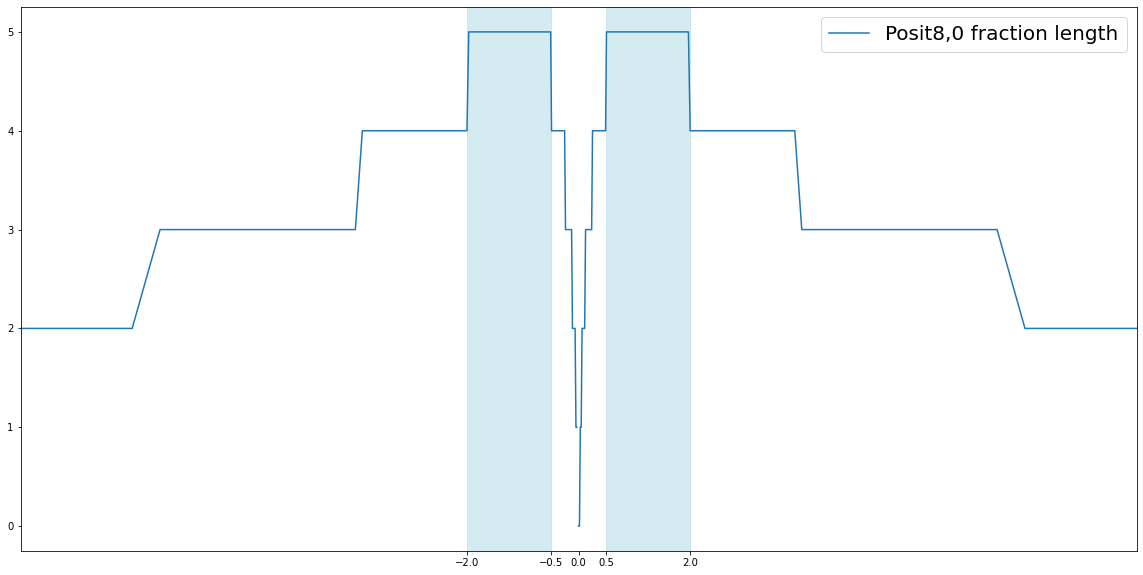
\includegraphics[width=\linewidth]{img/posit80fractionsWithZoom.png}
    \caption{\posit{8}{0} fraction length across the domain}
    \label{fig:posit80Fractions}
\end{figure}

Figure \ref{fig:posit80Fractions} shows this behaviour across the domain for a \posit{8}{0} configuration. In the plot we can see the region highlighted with the highest number of fraction bits with the associated real values $r \in [-1.9785,-0.5] \cup [0.5,1.9785]$


\begin{figure}
    \centering
    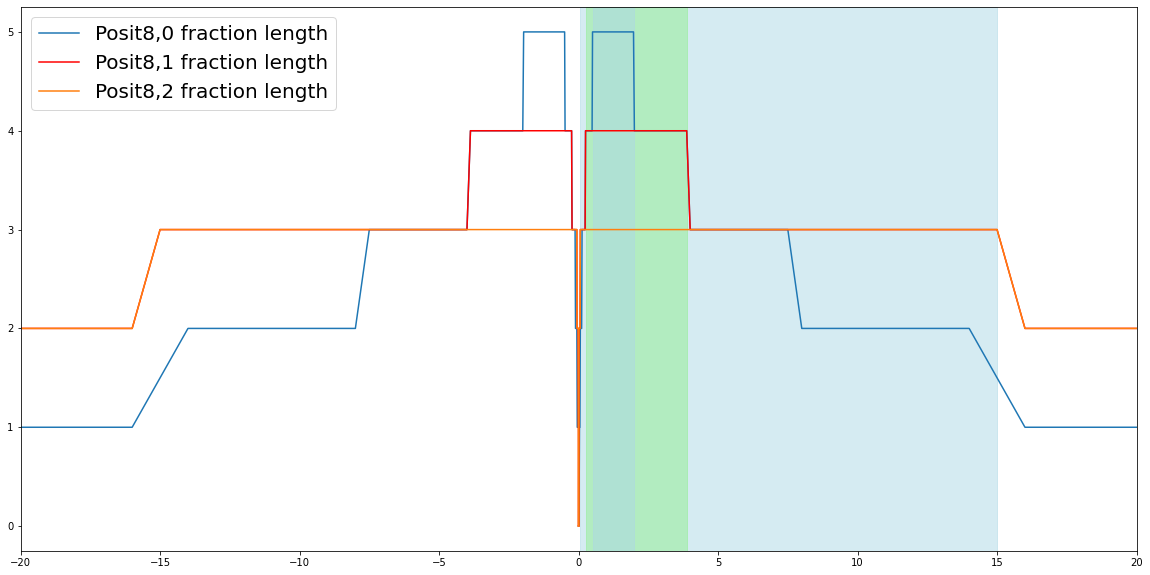
\includegraphics[width=\linewidth]{img/posit8xFractions.png}
    \caption{\posit{8}{x} fraction length comparison}
    \label{fig:posit8xFractions}
\end{figure}

Figure \ref{fig:posit8xFractions} shows the comparison of the fraction length between different configurations \posit{8}{[0,1,2]}. Obviously, if we allocate more bits for the exponent we are furtherly restricting the fraction bits, hence the different fraction bit lengths of the three configurations. However, with more exponent bits the range of maximum fraction bits is larger, despite containing the same number of distinct representations. This reflects on the format having a denser area of very high precision representation that thins out when we increase the exponent bits. 

We can generalize the range where the fraction has the highest amount of bits allocated:
\begin{equation}\label{eqn:highestFractionBits}
    \left [ \frac{1}{\text{useed}} , \text{useed} \right [ = \left [ \frac{1}{2^{2^{\text{esbits}}}}, 2^{2^{\text{esbits}}} \right [
\end{equation}

As we can see from Figure \ref{fig:posit8xFractions}, this range is always symmetric around the y-axis, so we have the two following ranges:
\begin{equation}\label{eqn:highestFractionBitsFull}
 \left ] -\text{useed}, -\frac{1}{\text{useed}} \right ]  ; \left [ \frac{1}{\text{useed}} , \text{useed} \right [ 
\end{equation}

Note that both in \eqref{eqn:highestFractionBits} and \eqref{eqn:highestFractionBitsFull}, the sets are open from the side of $\text{useed}$. This is because, by design, the last positive posit with the highest number of fraction bits is the one immediately preceding the posit representing $\text{useed}$.

\begin{table}
\caption{Ranges of the maximum fraction bits numbers for different posit configurations}
\label{tab:positXxMaxFractionRanges}
\centering
\begin{tabular}{c|rl}
Configuration               & Negative range                    & Positive range             \\ \hline
 \posit{8}{0}               & $[-1.96875, -0.5]$                  & $[0.5, 1.96875]$         \\
 \posit{8}{1}               & $[-3.875, -0.25] $                  & $[0.25, 3.875]$       \\
 \posit{8}{2}               & $[-15.0, -0.0625]   $               & $[0.0625, 15.0]$         \\
 \posit{16}{0}              & $[-1.9998779296875, -0.5]$          & $[0.5, 1.9998779296875]$ \\
 \posit{16}{1}              & $[-3.99951171875, -0.25] $          & $[0.25, 3.99951171875]$  \\
 \posit{16}{2}              & $[-15.99609375, -0.0625]$           & $[0.0625, 15.99609375]$ 
\end{tabular}
\end{table}

Table \ref{tab:positXxMaxFractionRanges} summarizes the ranges of maximum fraction length for different posit configurations. As we can see the range span depends on the exponent bits (\textit{esbits}), while the decimal accuracy of the range bounds depends on the total number of bits (\textit{nbits}).

Another useful concept to understand the behaviour of posits across their domain is the \textit{resolution}. Given a pair of consecutive posit representations $p_1, p_2 = p_1 + 1; p_1, p_2 \in \mathbb{Z}$, we define resolution the value:
\begin{equation}\label{eqn:positResolution}
    \overline{r} = r_2 - r_1
\end{equation}

Where $r_1,r_2 \in \mathbb{R}$ are the real values associated, respectively, to $p_1, p_2$. Resolution represents the inverse of \textit{density} of a given format in a given range of numbers: the lower the resolution, the closer the real values associated with two consecutive representations.

\begin{figure}
    \centering
    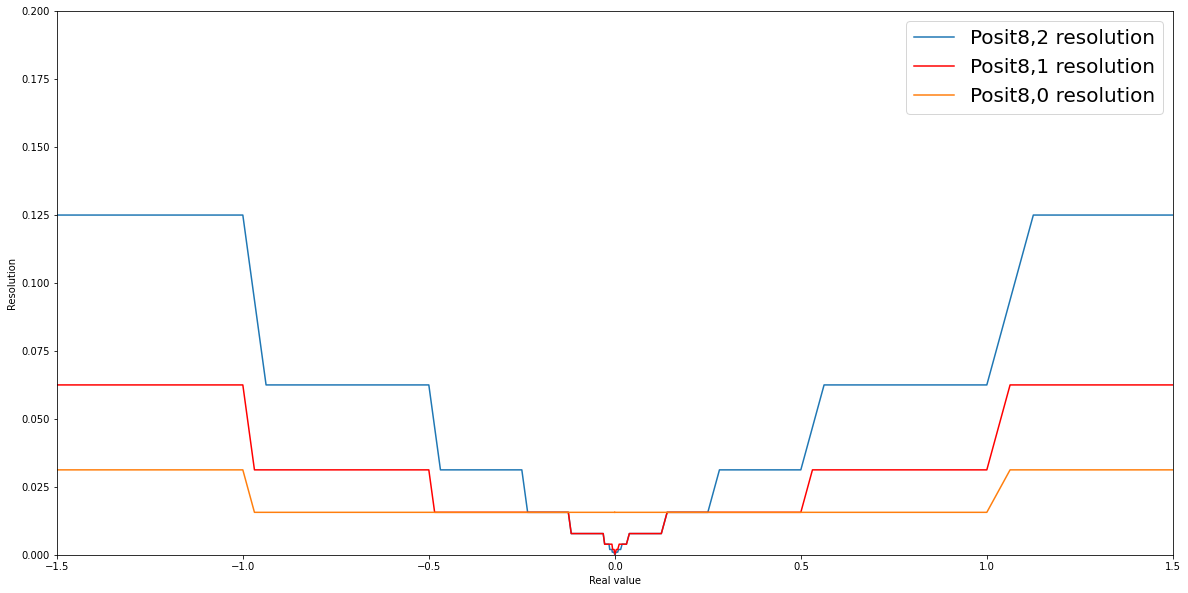
\includegraphics[width=\linewidth]{img/posit8xResolutions.png}
    \caption{\posit{8}{\{0,1,2\}} resolution across a portion of domain}
    \label{fig:posit8xResolutions}
\end{figure}

Figure \ref{fig:posit8xResolutions} shows the plot of $\overline{r}$ as function of $p_1$ for three configurations of \posit{8}{x}. As we can see, the \textit{resolution} decreases when approaching the value $0$ on the x-axis. Furthermore, the value of $\overline{r}$ is always smaller when using fewer exponent bits, this means that real numbers represented by successive posits are closer if compared to other posit configurations with a higher number of bits. As reported, the configurations for \posit{x}{0} have a flat resolution in the range $\left [ -1, 1 \right]$. This behaviour will be deeply analyzed in Section \ref{sec:Posit0bitExponent}.

\section{Posit and IEEE binary interoperability}\label{sec:fir}

One of the core concepts we deal with when bringing together the posit and the floating point domains is the interoperability between the two worlds. This means that we need to have two functions $f,g$ such that, given a set of Posits $\mathbb{P}$ and a set of floating point numbers $\mathbb{F}$:
\begin{equation}
    f: \mathbb{P} \xrightarrow[]{} \mathbb{F}
\end{equation}
\begin{equation}
    g: \mathbb{F} \xrightarrow[]{} \mathbb{P}
\end{equation}

Note that these two functions must be independent of the posit configuration \posit{nbits}{esbits} and the floating point type.

We introduce a \textit{float intermediate representation} (FIR) - i.e. a contact interface between any posit and any float configuration. Similarly to an IEEE binary, an FIR interface has three fixed-length fields:
\begin{itemize}
    \item sign $s_f$ on $1$ bit
    \item exponent $e_f$ on $\text{E}_f$ bits
    \item fraction $f_f$ on $\text{F}_f$ bits
\end{itemize}

Differently from the IEEE binary formats, the exponent here is a \textit{pure} one, without any offset applied. This means that the correspondent real value $r$ is:
\begin{equation}\label{eqn:firEquation}
    r = (-1)^{s_f} \cdot 2^{e_f} \cdot \left(1 + \frac{f_f}{2^{F_f}} \right)
\end{equation}

This interface allows us to decouple any posit configuration from any floating point configuration for conversion. Instead, we define another couple of functions $f_{fir}, 
g_{fir}$ that converts a posit into the FIR space and vice-versa.

On the other side, we need to provide another couple of functions for conversion between FIR and floating point space.

We can now characterize the two functions $f_{fir}, g_{fir}$ comparing Equations \eqref{eqn:positRealValue} and \eqref{eqn:firEquation}. If we take the general case from \eqref{eqn:positRealValue} and we expand the $useed$ term with \eqref{eqn:useed} we obtain:
\begin{equation}\label{eqn:positRealExpanded}
    r = (-1)^s_p \cdot 2^{2^{esbits} \cdot k + e_p} \cdot \left ( 1+ \frac{f_p}{2^{F_p}} \right)
\end{equation}

If we compare Equation \eqref{eqn:positRealExpanded} and \eqref{eqn:firEquation} we can impose equality on the three terms of the multiplication. The sign equality is straightforward: the sign of the number in FIR format must match the posit one.

If we are converting from posit to FIR, we can obtain the exponent $e_f$ as:
\begin{equation}
    e_f = 2^{esbits} \cdot k + e_p
\end{equation}

If we are converting the other way we can obtain $k$ and $e_p$ using modular arithmetic in base $2$: 
\begin{equation}
    k = e_f\ \mathbf{mod}\ 2^{esbits} = \left\lfloor \frac{e_f}{2^{esbits}} \right\rfloor
\end{equation},

\begin{equation}
    e_p = e_f\ \mathbf{rem}\ 2^{esbits}
\end{equation},
where $\mathbf{mod}$ is the integer division quotient and $\mathbf{rem}$ is the remainder.

For the fraction we need to impose the equality:
\begin{equation}\label{eqn:fractionalPartEquivalence}
    \frac{f_f}{2^{F_f}} = \frac{f_p}{2^{F_p}}
\end{equation}

Then we can solve for $f_f$ as:
\begin{equation}
    f_f = f_p \cdot 2^{F_f - F_p}
\end{equation}

and we can solve for $f_p$ as:
\begin{equation}
    f_p = f_f \cdot 2^{F_p - F_f}
\end{equation}

Note that, depending on the fraction sizes, the operation may result in loss of information, when we shrink a fraction with more bits to one with fewer bits.  Therefore, we need to take into account the bits we are discarding to eventually round the destination format according to their value.

So far, we have covered the conversion between FIR and posit numbers. The conversion between FIR and IEEE binary (or whichever floating point format) is similar, if not simpler.

Let us consider the IEEE binary32 conversion from/to a given FIR format. 

The exponent $e_{b32}$ of a binary32 number must be offset by $127$ during the transition between the two formats. Therefore, given $e_f$ the FIR exponent, we obtain:
\begin{equation}
    e_{b32} = e_f + 127
\end{equation}

On the other hand:
\begin{equation}
    e_{f} = e_{b32} - 127
\end{equation}

The fractional part can be handled as in \eqref{eqn:fractionalPartEquivalence}. Note that, differently from posit numbers, when the exponent is $0$, the fractional part of a binary32 needs to be interpreted without the leading $1.$ (i.e. the number must be considered as a subnormal).

Note that, the approach of using an intermediate representation can be used between whichever formats for real numbers that can be represented in the sign, exponent and fraction format.


\section{Generalized posits}

As seen in Figures \ref{fig:posit80Fractions} and \ref{fig:posit8xFractions}, the regime length has a sensible impact on the number of fraction bits we can use across the domain. Such length can change to the point that we do not have sufficient decimal accuracy (depending on the application) in a given range of numbers. 

An ideal approach would be to impose an upper limit to the regime length such that we can be sure that we will always reserve at least some bits for the fraction.

In \cite{9151086}, the authors propose a new way to characterize posit numbers. Additionally to the \textit{nbits}  and \textit{esbits} parameters, there are two (mutually exclusive) new parameters that control the dynamic range:
\begin{itemize}
    \item $K_b$: a regime bias 
    \item $rs$: a limit on the regime length
\end{itemize}

This results in having the maximum posit value shifted at:
\begin{equation}
    2^{2^{esbits} \cdot (k-K_b)}
\end{equation}

if using the $K_b$ parameter, or if we use the $rs$ parameter:
\begin{equation}
    2^{2^{esbits} \cdot rs} \cdot (1 - 2^{es - t - 1})
\end{equation}
where $ t = n - rs - 1$.


\section{A special case: 0-bit exponent}\label{sec:Posit0bitExponent}

In this section we focus on the posit format when configured with 0 exponent bits (i.e. \posit{x}{0}), also referring to our work in \cite{coco2020sensors}. If we impose $esbits = 0$ - that means also $es = 0$ - in \eqref{eqn:positRealValue}, we get:
\begin{equation}\label{eqn:positRealValueExp0}
    (-1)^s \cdot \text{2}^{k} \cdot \left ( 1+ \frac{f}{2^F} \right)
\end{equation}


\begin{figure}
    \centering
    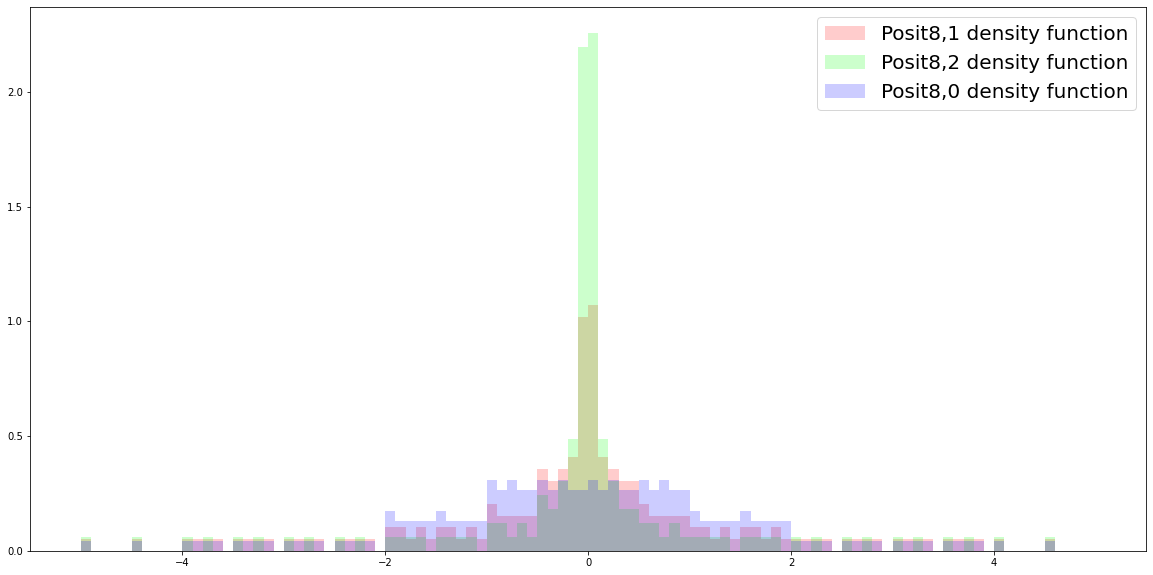
\includegraphics[width=\linewidth]{img/posit8xDensities.png}
    \caption{\posit{8}{x} density distribution around $0$.}
    \label{fig:posit8xDistributions}
\end{figure}

since $useed = 2^{2^0} = 2$. Having no exponent bits results in the behaviour shown in Figures \ref{fig:posit8xFractions} and \ref{fig:posit8xDistributions}. In particular, looking at Figure \ref{fig:posit8xDistributions}, the density distribution of a \posit{8}{0} tends to decay slower when moving away from the origin, thus having a better coverage in the range $[-useed,useed]$ when compared to posits with more exponent bits. This can be also seen in Figure \ref{fig:posit8xResolutions}, where the resolution of \posit{8}{0} is constant in $[-1,1]$ while the resolution of the other two posits increases also in this range. 

As we mentioned in the previous section, a 0-exponent bit posit in the range $[-1,1]$ has the property of having a constant resolution. 

We know that the fraction length $F_p$ depends on the regime length $l$ and, as a consequence, on the regime value $k$. In the range $[-1,1]$, we also know that the regime value is always $k \leq 0$, with the equality holding for posit representing real values of $\pm 1$. This means that in this region, the associated length (excluding the regime stop bit) is $l = - k$. Therefore, the fraction length $F$ can be written as $nbits - l - 2$, where $2$ includes the sign-bit and regime stop bit. We can rewrite \eqref{eqn:positRealValueExp0} as:
\begin{equation*}
    (-1)^s \cdot 2^k \cdot \left ( 1 + \frac{f_p}{2^{nbits + k - 2}} \right )
\end{equation*}

If we distribute the term $2^k$ inside the parenthesis we obtain:

\begin{equation*}
    (-1)^s \cdot \left ( 2^k + \frac{f_p\cdot 2^2}{2^{nbits}} \right )
\end{equation*}

\begin{equation*}
    (-1)^s \cdot \left ( \frac{2^{k+nbits}}{2^{nbits}} + \frac{f_p\cdot 2^2}{2^{nbits}} \right )
\end{equation*}

\begin{equation*}
    (-1)^s \cdot \left ( \frac{2^{k+nbits} + f_p\cdot 2^2}{2^{nbits}} \right )
\end{equation*}

\begin{equation*}
    (-1)^s \cdot \left ( \frac{2^2 \cdot (2^{k+ nbits - 2} + f_p)}{2^{nbits}} \right )
\end{equation*}

\begin{equation}\label{eqn:posit0exponentInUnitaryRange}
    (-1)^s \cdot \left ( \frac{2^2 \cdot (2^{F_p} + f_p)}{2^{nbits}} \right )
\end{equation}

Note that the value $2^{F_p} + f_p$ represents exactly the last $F_p + 1$ bits of the posit, since the fraction numerator $f_p$ is exactly $F_p$ bits long. Moreover, since the regime bits are in the format $000 \cdots 01$ and $2^{F_p}$ represents exactly the $1$ stopping bit, the integer $P$ representing the posit is exactly:
\begin{equation}\label{eqn:posit0expUnitary}
    P = 2^{F_p} + f_p
\end{equation}

Let us compare \eqref{eqn:posit0exponentInUnitaryRange} with \eqref{eqn:fixed2real}. In order to impose the equality between the two equations, $2^2 \cdot ( 2^{F_p} + f_p )$ must be equal to $f$ and $nbits$ must be equal to $F$ in \eqref{eqn:fixed2real}. Then, the integral part $i$ must be 0, since we are in the unitary range.

Therefore,  a \posit{x}{0} in the range $[-1,1]$ is equivalent to a fixed-point on $2\cdot x$ bits with a fractional part equal to $2^2 \cdot ( 2^{F_p} + f_p )$.

In practice, given a \posit{x}{0} we can just shift the posit representation two places left (hence the $2^2$ in \eqref{eqn:posit0exponentInUnitaryRange}) to obtain the fractional part of the correspondent fixed point number without any rounding.


\subsection{Fast arithmetic operation implementation
}\label{subsec:fastArithOps}

A format with $0$ exponent bits paves the way to implement several arithmetic operations in a way that does not require decoding of the posit itself, with the risk of introducing an approximation.

Hereafter, we will present the mathematical formulation of several functions, while in Section \ref{sec:cppPositCore} we will evaluate the performance and approximation error of such operations.

\subsubsection{Inverse}
 
Let us start with the reciprocating formulation:
\begin{equation}
    y = \frac{1}{x}
\end{equation}.

Firstly, we need to distinguish the formulations shown in \eqref{eqn:posit0exponentInUnitaryRange} from the range  $]-\infty,-1] \cup [1,\infty[$. When in this range, the regime value is always $k \geq 0$ ,  hence $l = k + 1$. This means that the number of bits for the fraction is $F = nbits - k - 3$. We can then write two different formulation for the real value associated to a \posit{x}{0}, where $r^- \in (-1,1)$ and $r^+ \in (-\infty, -1] \cup [1,\infty)$:
\begin{equation}
   r^- =  (-1)^s \cdot 2^k \cdot \left ( 1 + \frac{f_p}{2^{nbits + k - 2}} \right )
\end{equation},

\begin{equation}
   r^+ = (-1)^s \cdot 2^k \cdot \left ( 1 + \frac{f_p}{2^{nbits - k - 3}} \right )
\end{equation}.


\begin{figure}
    \centering
    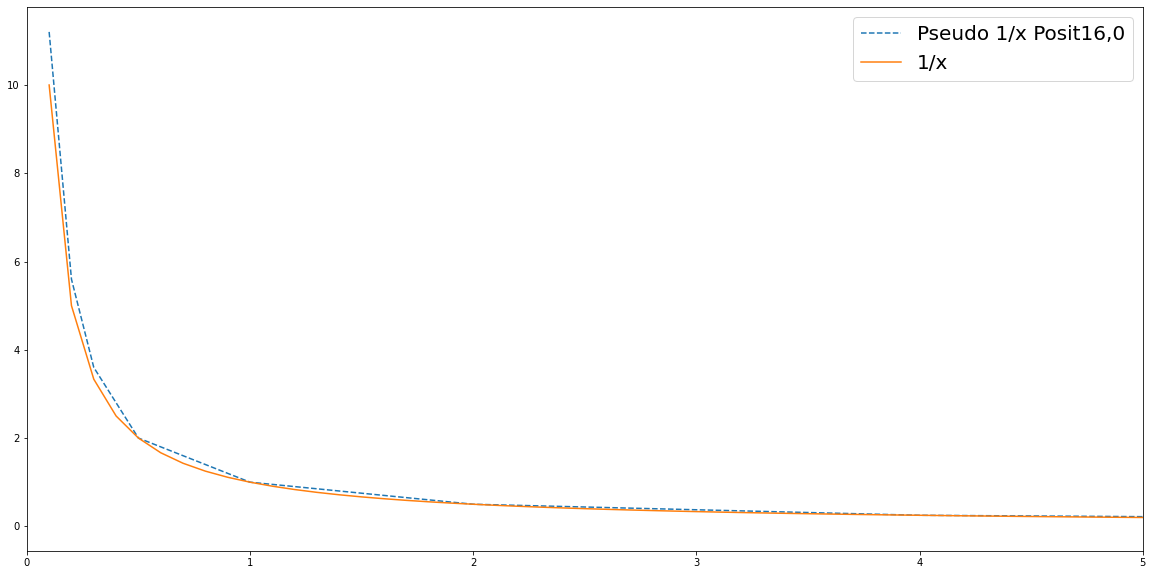
\includegraphics[width=\linewidth]{img/invPosit160.png}
    \caption{Comparison between exact inverse and decoding-free inverse for \posit{16}{0}}
    \label{fig:invPosit160}
\end{figure}

Now, let $x, y = \frac{1}{x}$ be two posits encoded with, respectively $s_x,k_x, f_x$ and $s_y = s_x, k_y, f_y$. Since there is an inversion, if $x \in [-1,1]$ then $y \in (-\infty, -1] \cup [1,\infty)$ (or vice-versa). We want to express $x \cdot y \sim 1$ using the posit representation of a real:
\begin{equation}\label{eqn:positx0prodInverse}
    x \cdot y = 2^{k_x+k_y} \cdot \left[ \left (1 + \frac{f_x}{2^{2^{nbits + k_x - 2}}} \right ) \cdot \left (1 + \frac{f_y}{2^{2^{nbits - k_y - 3}}} \right ) \right] \sim 1
\end{equation}.

We need to distinguish two cases:
\begin{itemize}
    \item[a)]$f_x = 0$, i.e. x is a pure exponential number and has an exact inversion in the posit space representation
    \item[b)] $f_x \neq 0$, i.e. x has also a fractional part and it has not an exact inversion in the posit space representation
\end{itemize}

Indicating with $P$ the integer representing the posit number, we can test the case as follows (i.e. the number is a pure exponential one if): 
\begin{equation}
    P\ \mathbf{and}\ (P - 1) = 0
\end{equation}.

\paragraph{Case a)} When in case a), we know that $k_y = -k_x$ (from inversion of \eqref{eqn:positRealValueExp0}). If we substitute this in \eqref{eqn:positx0prodInverse} we obtain:
\begin{equation}
    x \cdot y = 2^{0} \cdot \left[ \left (1 + \frac{f_x}{2^{2^{nbits + k_x - 2}}} \right ) \cdot \left (1 + \frac{f_y}{2^{2^{nbits + k_x - 3}}} \right ) \right] \sim 1
\end{equation}

We then develop the product inside the square brackets, discarding the product between the fraction themselves, introducing no approximation since $f_x = f_y = 0$:

\begin{equation}
    x \cdot y = 2^{0} \cdot \left[ 1 + \frac{f_x}{2^{2^{nbits + k_x - 2}}}  + \frac{f_y}{2^{2^{nbits + k_x - 3}}} \right] \sim 1
\end{equation}

Since the number must be equal to $1$, we impose the fractional part to be $0$, therefore:
\begin{equation}
    f_x + 2\cdot f_y = 0
\end{equation}

Since we already know that $f_x$ and $f_y$ are $0$, this holds by construction. 

Therefore, in this case the only transformation needed is $k_y = -k_x$. Since $k_x \leq 0$, changing the sign reflects on the length being increased by $1$. This means that the regime bits must be flipped and another bit of the same value must be appended to the regime. Since $f_x = 0$, if we invert it and add $1$ we get a bit set on the F-th least significant bit - i.e. on the former regime stop-bit. Wrapping everything up, we can obtain the inverse of $x$ with this expression, being $X$,$Y$ the integer numbers representing the posits:
\begin{equation}
    Y = X\ \mathbf{xor}\ (2^{nbits - 1} - 1) + 1
\end{equation}

\paragraph{Case b)} When in case b), $k_y = -k_x - 1$ (again from the inversion of \eqref{eqn:positRealValueExp0}). If we substitute this again \eqref{eqn:positx0prodInverse} we obtain:
\begin{equation}
    x \cdot y = 2^{-1} \cdot \left[ \left (1 + \frac{f_x}{2^{2^{nbits + k_x - 2}}} \right ) \cdot \left (1 + \frac{f_y}{2^{2^{nbits + k_x - 2}}} \right ) \right] \sim 1
\end{equation}

Again, we develop the product inside square brackets, discarding the fraction product, now introducing an approximation:

\begin{equation}
    x \cdot y = 2^{-1} \cdot \left[ 1 + \frac{f_x}{2^{2^{nbits + k_x - 2}}}  + \frac{f_y}{2^{2^{nbits + k_x - 2}}} \right] \sim 1
\end{equation}

Since the product must be $\sim 1$, we solve by $f_y$, obtaining:
\begin{equation}
\left\{\begin{matrix}
k_y = -k_x - 1 \\
f_y = 2^{F_x} - f_x
\end{matrix}\right.
\end{equation}

When changing the sign of $k_x$, we are acting like in case a), increasing the length of the regime by $1$ and changing its sign. However, now we also subtract $1$ from it, thus maintaining the regime length identical. This equals just flipping the regime bits.  For the fraction, we are subtracting an integer on $F_x$ bits - that is $f_x$ - from the value $2^F{_x}$. This again is equal to flipping $f_x$ bits and adding $1$. Since the case of $f_x = 0$ is not possible in b), this operation will never overflow $F_x$ bits, hence we can flip all the posit bits (excluding the sign) and add $1$. Wrapping everything up, let $X,Y$ be the integers representing the posits:

\begin{equation}
    Y = X\ \mathbf{xor}\ (2^{nbits - 1} - 1) + 1
\end{equation}.


We obtained that, in both cases a) and b), the formulation for the inversion is the same, so we can fuse the two into one. However, the second case introduces, inevitably, an approximation since we discarded the product between fractions inside the square brackets.


\subsubsection{$\mathbf{2\cdot x}$ and $\mathbf{x/2}$}

Let us proceed with the $y = 2\cdot x$ operation. For this operation we need to distinguish three ranges for the real value $r$:


\begin{itemize}
    \item[a)] $r \in (-0.5,0] \cup [0,0.5) \xrightarrow{} 2\cdot r \in (-1,1)$
    \item[b)] $r \in (-1,-0.5] \cup [0.5,1) \xrightarrow{} 2\cdot r \in (-2,-1] \cup [1,2) $
    \item[c)] $r \in (-\infty, -1] \cup [1, \infty)  \xrightarrow{} 2\cdot r \in (-\infty, -2] \cup [2, \infty)$
\end{itemize}

Regardless of the case we are in, we can write the following expression for the operation $y = 2 \cdot x$:

\begin{equation}
    y = 2 \cdot x = (-1)^{s_x} \cdot 2^{k_x + 1} \cdot \left(1 + \frac{f_x}{2^{F_x}} \right) 
\end{equation}

This means that, for all the cases, $k_y = k_x + 1$

For symmetry, we can focus only on the positive quadrant of the posit ring. The values $0.5,1,2$ are, respectively, represented by the integers $2^{nbits - 3}, 2^{nbits - 2}, 2^{nbits - 2} + 2^{nbits - 3}$.

\paragraph{Case a)} When $x \in [0,0.5)$ we know that $k_x \leq 0$, therefore $l_x = -k_x$. We also know that $y = 2\cdot x = \in [0,1)$, therefore $k_y \leq 0$ and $l_y = -k_y$. If we substitute the equivalence  $k_y = k_x + 1$ we obtain:
\begin{equation}
    l_y = - (k_x + 1) = l_x - 1
\end{equation}


In case a), we know that both $k_x, k_y$ will be in the form $000 \dots 01$. In particular, after multiplying by $2$, the regime length of $y$ will be shorter by 1. This corresponds to shifting the posit one position to the left. Since we are operating on positive numbers, we are guaranteed that the sign is preserved. Let $X,Y$ be the integer for the posits that represent $x,y$:
\begin{equation}
    Y = \mathbf{lls} (X,1) = 2 \cdot X
\end{equation}

where $\mathbf{lls}(X,N)$ is the logical left shift of the integer $X$ of $N$ positions.

\paragraph{Case b)} When $x \in [0.5,1)$ we know that $k_x \leq 0$ again. Hence, $l_x = -k_x$. In this case, $y = 2\cdot x \in [1,2)$, thus $k_y \geq 0$ and $l_y = k_x + 2$. Substituting the equivalence $k_y = k_x + 1$ we obtain:
\begin{equation}
    l_y = 2 - l_x
\end{equation}

Note that when $esbits = 0$, the range expressed in \eqref{eqn:highestFractionBits} is $[0.5,2)$ This means that $\forall x \in [0.5,2), l_x = 1$ and, as a consequence, we will always have $l_y = 2 - l_x = 1$. While $l_x = 1$ for a negative $k_x = -1$, $l_y = 1$ for a positive $k_y = 1$. This means that we need to flip the regime bits. Since we are in the region with the minimum number of regime bits (i.e. 2 regime bits, including the stopping bit), we just need to flip the 2 most significant bits (ignoring the sign). Let $X,Y$ be the integer for the posits that represent $x,y$:
\begin{equation}
    Y = X\ \mathbf{xor}\ (2^{nbits - 2} + 2^{nbits - 3})
\end{equation}


\paragraph{Case c)} When $x \in [1,\infty)$ we know that both $k_x \geq 0$ and $k_y \geq 0$. Therefore, $l_x = k_x + 1$ and $l_y = k_y + 1$. Substituting the equivalence $k_y = k_x + 1$ we obtain:
\begin{equation}
    l_y = l_x + 1
\end{equation}

In this case, the regime bits are in the format $111 \cdots 10$. When we multiply by two we are increasing the regime and the regime length by $1$. This means that we need to put a single bit set in front of the regime and then shift the posit to the right (possibly discarding the fraction least significant bit). Let $X,Y$ be the integer for the posits that represent $x,y$:
\begin{equation}
    Y = (X\ \mathbf{or}\ 2^{nbits - 1}) \cdot 2^{-1}
\end{equation}

Note that we can elaborate in the same way for the $x/2$ operation: this case is omitted because it is symmetrical to the previous one and symmetrical would be the results obtained. 



\subsubsection{Unitary complement: $\mathbf{1-x}$}

Suppose we are in the $[0,1]$ range and we want to perform the \textit{unitary complement} of a number $x$, that is:
\begin{equation}
    y = 1 - x    
\end{equation}

As seen before in \eqref{eqn:posit0expUnitary}, in the unitary range the posit integer $P = 2^{F_p} + f_p$. 

To derive an expression for this complement operation we can write $x + y = 1$ and expand the terms:
\begin{equation}
    2^{k_x} \cdot \left(1 + \frac{f_x}{2^{F_x}} \right) + 2^{k_y} \cdot \left(1 + \frac{f_y}{2^{F_y}} \right) = 1
\end{equation}

When in the unitary range we already know that $k \leq 1$ and $F = nbits - 2 + k$ for both $x$ and $y$. If we substitute this in both the terms of the addition we obtain:
\begin{equation}
    2^{k_x} + \ 2^{k_y} + \frac{f_x + f_y}{2^{nbits - 2}} = 1
\end{equation}

We multiply both sides by $2^{nbits - 2}$ obtaining:
\begin{equation}
    2^{F_x} + 2^{F_y} + f_x + f_y = 2^{nbits - 2}
\end{equation}

We then apply  \eqref{eqn:posit0expUnitary}, obtaining the expression needed to compute $y = 1 - x$:
\begin{equation}
    X + Y = 2^{nbits - 2} \xrightarrow{} Y = 2^{nbits - 2} - X
\end{equation}



\subsubsection{Sigmoid}
\begin{figure}
    \centering
    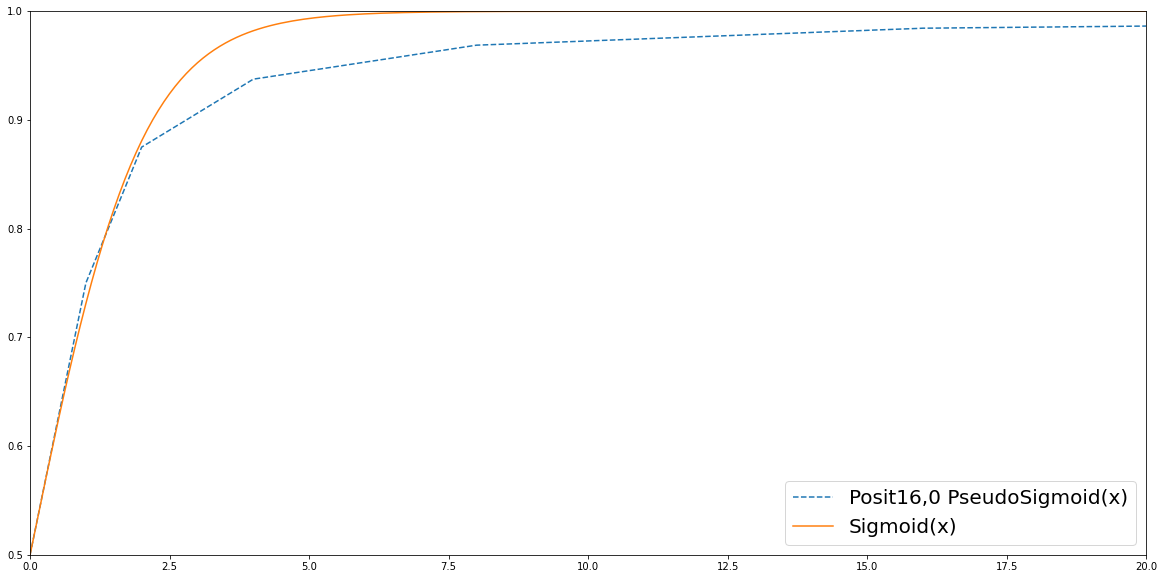
\includegraphics[width=\linewidth]{img/sigmoidPosit160.png}
    \caption{Actual sigmoid vs plot of the integer representation of a \posit{16}{0}}
    \label{fig:posit160Sigmoid}
\end{figure}

In \cite{gustafson2017beating}, John L. Gustafson et al. observed a particular property of the posit representation when plotting the integer value representing the posit and the correspondent real value.

The sigmoid curve is a very well-known activation function for neural networks:
\begin{equation}
    \mathbf{sigmoid}(x) = \frac{1}{1 + e^{-x}}
\end{equation}

If we look at Figure \ref{fig:posit160Sigmoid} we can see that the actual sigmoid curve is very similar to the curve obtained by plotting the value of the integer $P$ representing a posit $p$ for any correspondent real value $r$. However, the plot for $P$ must be scaled and translated to match the sigmoid output in $[0,1]$. The scaling and translation are performed as follows: let $\hat{S}(x)$ be the \textit{pseudo-sigmoid} shown in figure \ref{fig:posit160Sigmoid}, and $X$ the integer representing the posit associated to the real value $x$:
\begin{equation}
    \hat{S}(x) = \frac{X}{2^{nbits}} + \frac{1}{2}
\end{equation}

In \cite{gustafson2017beating} the authors reported another version of this transformation, obtaining the posit integer representation for the sigmoid output from the posit integer representation of its input. Let $Y$ be the integer posit representation for the sigmoid $\hat{S}(x)$ and $X$ the posit integer representation associated to the real value $x$:
\begin{equation}\label{eqn:pseudoSigmoidPosit0}
    Y = \left ( 2^{nbits - 2} + \frac{X}{2} \right ) \cdot \frac{1}{2}
\end{equation}

As pointed out in \cite{coco2020sensors}, the two expressions are equivalent.

\subsubsection{Hyperbolic tangent}

\begin{figure}
    \centering
    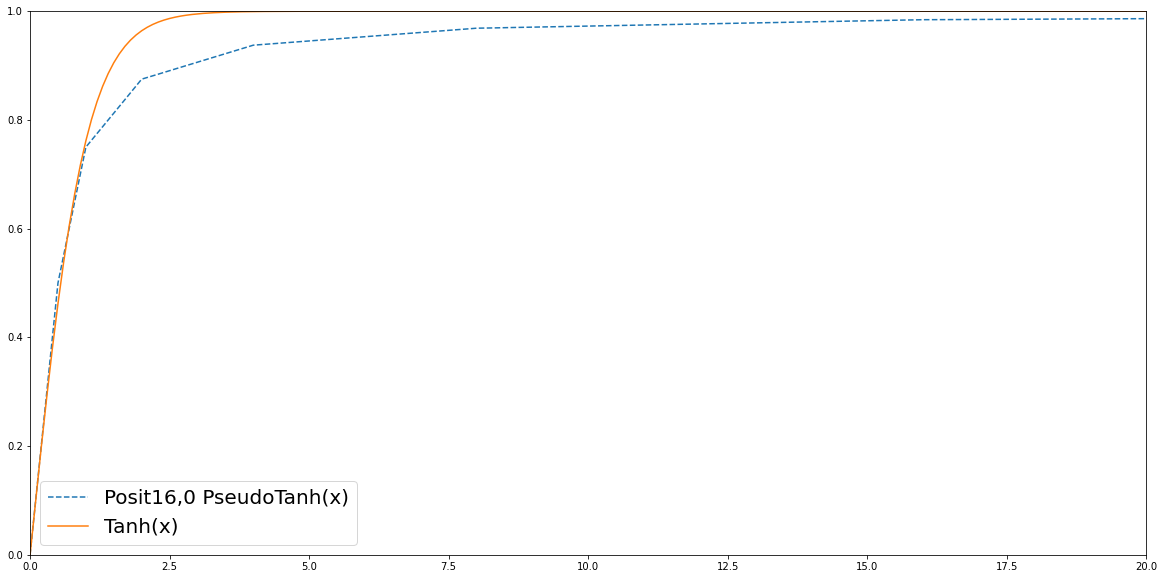
\includegraphics[width=\linewidth]{img/tanhPosit160.png}
    \caption{Hyperbolic tangent comparison between actual and pseudo version.}
    \label{fig:pseudoTanhPosit0}
\end{figure}

The hyperbolic tangent is another commonly used activation function in neural networks. Its expression is quite similar to the sigmoid:
\begin{equation}
    \mathbf{tanh}(x) = \frac{e^{2x}-1}{e^{2x}+1} 
\end{equation}

We can obtain this expression from the sigmoid by applying a scale and a transformation:

\begin{equation}
   \mathbf{tanh}(x) =  2 \cdot \mathbf{sigmoid}(2 \cdot x) - 1
\end{equation}

We can rework the previous expression as follows:
\begin{equation}
    \mathbf{tanh}(x) = - ( 1 - 2\cdot \mathbf{sigmoid}(2\cdot x))
\end{equation}

Suppose we only consider negative values for $x$ for symmetry. We know that the $2\cdot x$ operation can be done without decoding with \posit{x}{0}. Since we are dealing with negative numbers, the output of the sigmoid will be in $[0,1/2]$. Again, multiplying this number by $2$ can be done without decoding the posit and the output will be in $[0,1]$. Therefore, we can apply the $1-y$ operation without decoding the posit. Finally, we can change the sign with a 2's complement of the representation.

If we substitute the sigmoid with the pseudo-sigmoid seen in \eqref{eqn:pseudoSigmoidPosit0} we obtain a decoding-free \textit{pseudo hyperbolic tangent}.

\subsubsection{Extended Linear Unit}

\begin{figure}
    \centering
    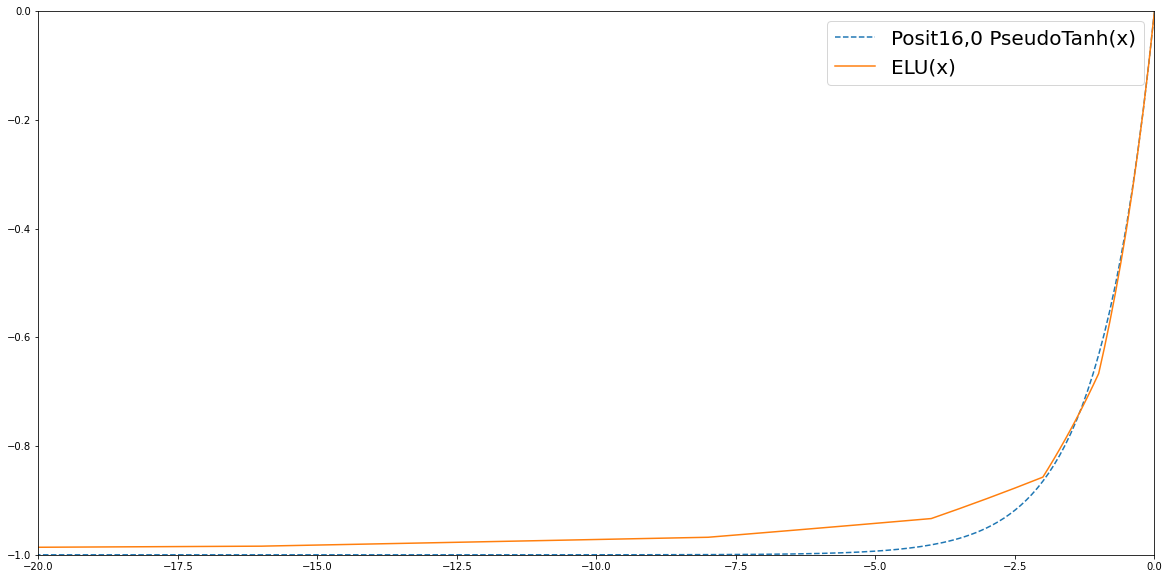
\includegraphics[width=\linewidth]{img/eluPosit160.png}
    \caption{ELU comparison between actual and pesudo version.}
    \label{fig:pseudoEluPosit0}
\end{figure}


The Extended Linear Unit (ELU) is another commonly used activation function in neural networks, mainly adopted to avoid vanishing gradients of S-shaped functions like a sigmoid and hyperbolic tangent.

The formulation of the ELU function is the following:

\begin{equation}
\mathbf{elu}(x)=\left\{\begin{matrix}
x & x \geq 0 \\
\alpha \cdot (e^x - 1) & x < 0  \\
\end{matrix}\right.
\end{equation}

The case for $x \geq 0$ is straightforward, so we focus on the $\alpha \cdot (e^x - 1)$ part. In particular, we consider the case where $\alpha = 1$, hence:
\begin{equation}
    \mathbf{elu}(x) = (e^x - 1) = 2 \cdot \left [ \frac{1}{2\cdot \mathbf{sigmoid}(-x)} - 1 \right]
\end{equation}

We can start from the sigmoid obtained before. We firstly negate the argument to have a sigmoid output in $[0.5,1]$. We can then invert without decoding obtaining an output in $[1,2]$. This output is divided by $2$, obtaining an output in $[0.5,1]$. We can apply the $1-y$ operation without decoding and then multiply everything by $2$ to obtain the final result in \eqref{eqn:sigm_twinvm1}.

\begin{align}
   \label{eqn:sigm_mx}\textnormal{sigmoid}(-x) = \frac{1}{1+e^{x}}  & \\
   \label{eqn:sigm_invx}1/\textnormal{sigmoid}(-x) = 1+e^x & \\
   \label{eqn:sigm_invtw}1/(2\cdot\textnormal{sigmoid}(-x)) = \frac{1+e^x}{2}& \\
   \label{eqn:sigm_invm1}1/(2\cdot\textnormal{sigmoid}(-x))-1 = \frac{1+e^x}{2} - 1 = \frac{e^x-1}{2} & \\
  \label{eqn:sigm_twinvm1}2\cdot[1/(2\cdot\textnormal{sigmoid}(-x))-1] = e^x -1&
\end{align}

If we substitute the sigmoid function with the pseud-sigmoid seen in \eqref{eqn:pseudoSigmoidPosit0} we obtain a decoding-free \textit{pseudo-ELU}.




\section{Arithmetic operations on posits}\label{sec:posit_ops}

In this section, we cover the different phases of binary operations between posits.

\subsection{Input conditioning and posit decoding}\label{input_conditioning_section}

Before the decoding of the posit operands, we make use of some logic meant to discriminate different cases of posit configurations. These are those cases where either one of the operands is $0$ (i.e. actual $0$ and NaR), or when the operation leads to straightforward output. All these cases can be reduced to simple ones that, similarly to the \textit{fast operations}, can be resolved without decoding the posit value. Handling these conditions upfront is important since it simplifies the rest of the logic for the operations.

\hypertarget{special_cases_link}{~}
\textit{special} and \textit{trivial} cases are those where, respectively:
\begin{itemize}
\item one of the inputs is \textit{special} (e.g. NaR or inf), which leads to a \textit{special} output
\item the output of a given operation is \textit{special} and this can be directly inferred from the inputs (e.g. division by zero).
\end{itemize}


If one of these cases is caught, the result is produced without decoding.


The possible combinations, for each of the four operation, are tabulated in \ref{table:table_posit_op_combination}, with a distinction between \textit{special} and \textit{trivial} cases.

Special cases are colored in \textcolor{red}{red}, and trivial are colored in \textcolor{orange}{orange}.
Each posit value can either be \textit{special}, i.e. $\in \{0$, \mbox{NaR}\}, or \textit{non-special}.

\begin{table}
\begin{center}
\begin{tabular}{ cc }   % top level tables, with 2 columns
addition & subtraction \\
\begin{tabular}{||c c c | c||}
    \hline
    $p_1$ & op & $p_2$ & $p_{out}$ \\ [0.5ex]
    \hline\hline
    $0$ & $+$ & $0$ & \textcolor{red}{$0$} \\
    \hline
    $0$ & $+$ & NaR & \textcolor{red}{NaR} \\
    \hline
    $0$ & $+$ & $p_2$ & \textcolor{yellow}{$p_2$} \\ %%%% https://www.overleaf.com/learn/latex/Using_colours_in_LaTeX
    \hline
    NaR & $+$ & $0$ & \textcolor{red}{NaR} \\
    \hline
    NaR & $+$ & NaR & \textcolor{red}{NaR} \\
    \hline
    NaR & $+$ & $p_2$ & \textcolor{red}{NaR} \\
    \hline
    $p_1$ & $+$ & $0$ & \textcolor{yellow}{$p_1$} \\
    \hline
    $p_1$ & $+$ & NaR & \textcolor{red}{NaR} \\
    \hline
    $p_1$ & $+$ & $p_2$ & \textcolor{green}{$p_1 + p_2$} \\
    \hline %%% 2 more trivial cases
    $p_1$ & $+$ & $-p_1$ & \textcolor{yellow}{$0$} \\
    \hline
    $-p_2$ & $+$ & $p_2$ & \textcolor{yellow}{$0$} \\
    \hline
\end{tabular} &
\begin{tabular}{||c c c | c||}
    \hline
    $p_1$ & op & $p_2$ & $p_{out}$ \\ [0.5ex]
    \hline\hline
    $0$ & $-$ & $0$ & \textcolor{red}{$0$} \\
    \hline
    $0$ & $-$ & NaR & \textcolor{red}{NaR} \\
    \hline
    $0$ & $-$ & $p_2$ & \textcolor{yellow}{$-p_2$} \\ %%%% https://www.overleaf.com/learn/latex/Using_colours_in_LaTeX
    \hline
    NaR & $-$ & $0$ & \textcolor{red}{NaR} \\
    \hline
    NaR & $-$ & NaR & \textcolor{red}{NaR} \\
    \hline
    NaR & $-$ & $p_2$ & \textcolor{red}{NaR} \\
    \hline
    $p_1$ & $-$ & $0$ & \textcolor{yellow}{$p_1$} \\
    \hline
    $p_1$ & $-$ & NaR & \textcolor{red}{NaR} \\
    \hline
    $p_1$ & $-$ & $p_2$ & \textcolor{green}{$p_1 - p_2$} \\
    \hline %%% 2 more trivial cases
    $p_1$ & $-$ & $p_1$ & \textcolor{yellow}{$0$} \\
    \hline
    $p_2$ & $-$ & $p_2$ & \textcolor{yellow}{$0$} \\
    \hline
\end{tabular}\\ \\
\end{tabular}
\end{center}
\begin{center}
\begin{tabular}{ cc }   % top level tables, with 2 columns
multiplication & division \\
\begin{tabular}{||c c c | c||}
    \hline
    $p_1$ & op & $p_2$ & $p_{out}$ \\ [0.5ex]
    \hline\hline
    $0$ & $*$ & $0$ & \textcolor{red}{$0$} \\
    \hline
    $0$ & $*$ & NaR & \textcolor{red}{NaR} \\
    \hline
    $0$ & $*$ & $p_2$ & \textcolor{yellow}{$0$} \\ %%%% https://www.overleaf.com/learn/latex/Using_colours_in_LaTeX
    \hline
    NaR & $*$ & $0$ & \textcolor{red}{NaR} \\
    \hline
    NaR & $*$ & NaR & \textcolor{red}{NaR} \\
    \hline
    NaR & $*$ & $p_2$ & \textcolor{red}{NaR} \\
    \hline
    $p_1$ & $*$ & $0$ & \textcolor{yellow}{$0$} \\
    \hline
    $p_1$ & $*$ & NaR & \textcolor{red}{NaR} \\
    \hline
    $p_1$ & $*$ & $p_2$ & \textcolor{green}{$p_1 * p_2$} \\
    \hline
\end{tabular} &
\begin{tabular}{||c c c | c||}
    \hline
    $p_1$ & op & $p_2$ & $p_{out}$ \\ [0.5ex]
    \hline\hline
    $0$ & $/$ & $0$ & \textcolor{red}{NaR} \\
    \hline
    $0$ & $/$ & NaR & \textcolor{red}{NaR} \\
    \hline
    $0$ & $/$ & $p_2$ & \textcolor{yellow}{$0$} \\ %%%% https://www.overleaf.com/learn/latex/Using_colours_in_LaTeX
    \hline
    NaR & $/$ & $0$ & \textcolor{red}{NaR} \\
    \hline
    NaR & $/$ & NaR & \textcolor{red}{NaR} \\
    \hline
    NaR & $/$ & $p_2$ & \textcolor{red}{NaR} \\ %%%%
    \hline
    $p_1$ & $/$ & $0$ & \textcolor{yellow}{NaR} \\
    \hline
    $p_1$ & $/$ & NaR & \textcolor{red}{NaR} \\
    \hline
    $p_1$ & $/$ & $p_2$ & \textcolor{green}{$p_1 / p_2$} \\
    \hline
\end{tabular} \\
\end{tabular}
\end{center}
\caption{Table operation cases for any posit combination}
\label{table:table_posit_op_combination}
\end{table}







In order to simplify the logic concerning addition/subtraction, we can already enforce an order between the inputs, so that $p_1$ and $p_2$ carry, respectively, the largest and smaller value (in absolute terms). At the same time, we reserve a flag indicating whether the sign of the two numbers is concordant or not. This observation will be used from now on to simplify the reasoning on the operational implementation.




In the following sections, we cover the implementation of Posit binary operations. For simplicity we will refer to the real value of a posit as follows:
\begin{equation}\label{eqn:posit_equation}
    p = (-1)^{s} \cdot 2^{te} \cdot (1.f)
\end{equation}
Where $te$ is the exponent-regime joint value:
\begin{equation}
    te = (2^{2^{esbits}})^{k} \cdot 2^{e} = 2^{2^{esbits}\cdot k + e}
\end{equation}

\subsection{Addition and Subtraction}\label{Addition_and_Subtraction}

Due to the similarities between the addition and subtraction operations, we will discuss their implementation together, highlighting where the two operations differ.


Given two posits, $p_1$ and $p_2$, expressed as \eqref{eqn:posit_equation}, the goal is to find the tuple $(s_{out}, k_{out}, e_{out}, f_{out})$ such that the following holds:
\begin{equation}\label{equ:addition_equation_001}
    \underbrace{\big[ (-1)^{s_1} \cdot 2^{te_1} \cdot (1.f_1) \big]}_{p_1} \pm \underbrace{\big[ (-1)^{s_2} \cdot 2^{te_2} \cdot (1.f_2) \big]}_{p_2} = \underbrace{ (-1)^{s_{out}} \cdot \overbrace{\big(2^{2^{esbits}}\big)^{k_{out}} \cdot 2^{e_{out}}}^{2^{te_{out}}} \cdot (1.f_{out})}_{p_{out}}
\end{equation}

We can generalize for rounding inexactness, obtaining the following:

\begin{equation}
\begin{gathered}
    (s_{out}, k_{out}, e_{out}, f_{out}): \\
    \min | \big[ (-1)^{s_1} \cdot 2^{te_1} \cdot (1.f_1) \pm (-1)^{s_2} \cdot 2^{te_2} \cdot (1.f_2) \big] - \big[ (-1)^{s_{out}} \cdot 2^{te_{out}} \cdot (1.f_{out}) \big] |
\end{gathered}
\end{equation}


The following always requires that
\begin{equation}\label{equ:p1_greater_p2}
|p_1| \ge |p_2|
\end{equation}
and they are not  is \textit{special}.
A constant $b$ (as in \textit{bias}) is defined as
\begin{equation}\label{equ:b_bias}
\begin{aligned}
% b & = \big( 2^{es} \cdot k_1 + e_1 \big) - \big( 2^{es} \cdot k_2 + e_2 \big) \\
%   & = te_1 - te_2 \geq 0
b \triangleq te_1 - te_2
\end{aligned}
\end{equation}
Given (\ref{equ:p1_greater_p2}) $b \ge 0$, and $s_{out} \leftarrow s_1$. $te_2$ is expanded to $te_1 - (te_1 - te_2)$ so that $2^{te_2}$ becomes $2^{te_1} \cdot 2^{-b}$ and the scale factor $2^{te_1}$ can be brought out. Finally, the left-hand side of (\ref{equ:addition_equation_001}) can be simplified to
\begin{equation}
(-1)^{s_1} \cdot 2^{te_1} \cdot \big[ \underbrace{(1.f_1) \pm (1.f_2) \cdot 2^{-b}}_{1.f_{out}}\big]
\end{equation}
which can be interpreted also as a sequence of bit-wise operations.
Then, we handle the fractional components; we sum them together, considering that the notation $(1.f)_2$\footnote{using explicit subscript notation to notify the base} encapsulates all the numbers $F_i \in [(1.0)_2, (1.111\dots)_2 ] \equiv [1.0_{10},  2.0_{10})$.

The factor $2^{-b}$ applies a right shift to $(1.f)_2$ by $b$ positions:
$$
(1.f)_2 \cdot 2^{-b} \equiv (\underbrace{0.0000\dots0000}_{b}1f)_2 \in (0.0_{10}, 1.0_{10}]
$$



Therefore, the addition and subtraction operations can generate values respectively in the range of:
\begin{itemize}
    \item \textit{addition}: $(1.f_1) + [(1.f_2) \cdot 2^{-b}] \in [1, 4)^{*}$
    \item \textit{subtraction}: $(1.f_1) - [(1.f_2) \cdot 2^{-b}] \in [0, 2)^{**}$
\end{itemize}
We can interpret them as fixed point numbers \texttt{Fx<2,\_>} and \texttt{Fx<1,\_>}\footnote{\texttt{\_} signifying undetermined a priori fixed point total size}, where $2$ and $1$ are the number of bits required to represent the largest integers $3^{*}$ and $1^{**}$.

This is is where the addition and subtraction flow slightly diverge: in order to re-normalize the result of the fractional addition/subtraction into the $(1.f_{out})$ configuration we have two different approaches:

    \subsubsection{Addition}
    the fraction is shifted right by $1$ if the most significant bit is $1$, i.e. $(1.f_1) + (1.f_2) \cdot 2^{-b} \ge 2.0$. 
    This drops the least significant bit which is useless if such a bit is a $0$. Otherwise, if it's a $1$ the information regarding such loss must be preserved and used later on: for that a signal named \textit{is\_truncated} is used. Finally, the right shift is matched in the exponent by increasing the value $te$ by 1.
    \subsubsection{Subtraction}
    the fraction must be shifted left by a variable amount ($lz$), i.e. the number of leading zeros, for normalization. This is where the second instance of the leading-zero-counter is employed (besides the one used for the decoding). The exponent compensation is done by decreasing the value $te$ by the number of leading zeros.
    $$
    2^{te} \cdot (\overbrace{0.00\dots00}^{lz}1f) \equiv 2^{te - lz} \cdot (1.f)
    $$

\begin{figure}
    \begin{center}
    % \includegraphics[height=0.7\textheight]{assets/figures/addition_flow.pdf}
    \includegraphics[width=\textwidth]{figures/addition_flow.pdf}
    \caption{Posit algebraic sum algorithmic flow}
    \label{fig:additionflow}
    \end{center}
\end{figure}

An example of the algorithmic flow for the posit algebraic sum is shown in Figure \ref{fig:additionflow}.

\subsection{Multiplication}\label{Multiplication}

As before, we have two posit expressed as (\eqref{eqn:posit_equation}); the goal is finding the tuple $(s_{out},$ $k_{out}, e_{out}, f_{out})$ such that:


\begin{equation}\label{equ:multiplication_equation_001}
    \big[ (-1)^{s_1} \cdot 2^{te_1} \cdot (1.f_1) \big] \cdot \big[ (-1)^{s_2} \cdot 2^{te_2} \cdot (1.f_2) \big] =(-1)^{s_{out}} \cdot \overbrace{\big(2^{2^{ES}}\big)^{k_{out}} \cdot 2^{e_{out}}}^{2^{te_{out}}} \cdot (1.f_{out})
\end{equation}

Again, we need to consider rounding inexactness:

\begin{equation}
\begin{gathered}
    (s_{out}, k_{out}, e_{out}, f_{out}): \\
    \min \left| \big[ (-1)^{s_1} \cdot 2^{te_1} \cdot (1.f_1) \cdot (-1)^{s_2} \cdot 2^{te_2} \cdot (1.f_2) \big] - \big[ (-1)^{s_{out}} \cdot 2^{te_{out}} \cdot (1.f_{out}) \big] \right|
\end{gathered}
\end{equation}
Simplifying the equation, we obtain the following:
\begin{equation}
\begin{gathered}
    (-1)^{s_1 \oplus s_2}  \cdot \big[ 2^{te_1} \cdot 2^{te_2} \big] \cdot \big[ (1.f_1) \cdot (1.f_2) \big]
\end{gathered}
\end{equation}

Where $s_1$ and $s_2$ are \textit{xor}-ed together to get the sign $s_{out}$ and the total exponents $te_1$ and $te_2$ summed up to give $te_{out}$. 
$(1.f_1) \cdot (1.f_2)$ results in a number $\in [1, 4)$, and just like in the addition -- if not already -- it is readjusted to its normalized format by means of a right-shift and an increment of $te$.


\begin{figure}
    \begin{center}
    % \includegraphics[height=0.7\textheight]{assets/figures/posit_mul_flow.pdf}
    \includegraphics[width=\textwidth]{figures/posit_mul_flow.pdf}
    \caption{Posit multiplication algorithmic flow}
    \label{fig:mulflow}
    \end{center}
\end{figure}

An example of the algorithmic flow for the posit algebraic sum is shown in Figure \ref{fig:mulflow}.

\subsection{Division}



Similarly to the addition/subtraction and multiplication, we have two posit expressed as (\eqref{eqn:posit_equation}), the goal is finding the tuple $(s_{out}, k_{out}, e_{out}, f_{out})$ such that
the following holds:
\begin{equation}\label{equ:division_equation_001}
    \frac{\big[ (-1)^{s_1} \cdot 2^{te_1} \cdot (1.f_1) \big]}{\big[ (-1)^{s_2} \cdot 2^{te_2} \cdot (1.f_2) \big]} = (-1)^{s_{out}} \cdot \overbrace{\big(2^{2^{ES}}\big)^{k_{out}} \cdot 2^{e_{out}}}^{2^{te_{out}}} \cdot (1.f_{out})
\end{equation}

Again, we can account for rounding inexactness:


\begin{equation}
\begin{gathered}
    (s_{out}, k_{out}, e_{out}, f_{out}): \\
    \min \left| \frac{ (-1)^{s_1} \cdot 2^{te_1} \cdot (1.f_1)}{(-1)^{s_2} \cdot 2^{te_2} \cdot (1.f_2)} - \big[ (-1)^{s_{out}} \cdot 2^{te_{out}} \cdot (1.f_{out}) \big] \right|
\end{gathered}
\end{equation}
Simplifying the left-hand side of (\ref{equ:division_equation_001}), we obtain
\begin{equation}
\begin{gathered}
    \frac{(-1)^{s_1}}{(-1)^{s_2}} \cdot \frac{2^{te_1}}{2^{te_2}} \cdot \frac{(1.f_1)}{(1.f_2)}
\end{gathered}
\end{equation}
which identically to the multiplication, suggests that $s_{out} = s_1 \oplus s_2$ and $te_{out} = te_1 - te_2$.
From the mathematical standpoint it comes off as not too dissimilar than a product, as seen in section \ref{Multiplication}; the only difference is the result falling within the range
\begin{equation}\label{equ:min_max_frac_0010032}
\begin{aligned}
\left[\min{\frac{(1.f_1)}{(1.f_2)}}, \max{\frac{(1.f_1)}{(1.f_2)}} \right] &= \left[\frac{\min{(1.f_1)}}{\max{(1.f_2)}}, \frac{\max{(1.f_1)}}{\min{(1.f_2)}} \right] = \\
&= \left[\frac{1.0}{2.0^{-}}, \frac{2.0^{-}}{1.0} \right] =\\
&= \left(0.5, 2.0 \right) = \\
&= \left[(0.111\dots)_2, (1.111\dots)_2 \right]
\end{aligned}
\end{equation}
range rather than the product's $[1.0, 4.0)$ range.


If we remember that $(1.f)$ is does not belong to $\mathbb{R}$, but rather to $ \mathbb{Q}$, we can multiply both numerator and denominator such that they are two integer numbers:
\begin{equation}\label{divunsignedinteger00001}
\frac{1.\overbrace{011\dots0001001}^{F-bits}}{1.\underbrace{110\dots0001111}_{F-bits}} \equiv \frac{1011\dots0001001 \cdot \cancel{2^{-F}}}{1110\dots0001111 \cdot \cancel{2^{-F}}}
\end{equation}
and the result is the one of an integer division. Consequence of (\ref{equ:min_max_frac_0010032}), the result will have either a $0$ or $1$ as most significant bit. 

The critical part of the division operation is the one in Equation \eqref{divunsignedinteger00001}. Integer division can be performed in different ways, each with a trade-off between accuracy and resulting hardware complexity. We will deepen on this topic in Section \ref{Approximated_Algorithms}. 




\subsection{Normalization}


\textit{Normalization} consists in the conversion of a general FIR representation, i.e. the output of sum, multiplication or division, to a posit bit-string. This is typically independent of the operation computed before.


The two terms $k'$ and $e$ must be unpacked from the total exponent ($te$) term (\eqref{eqn:posit_equation}):
\begin{equation}\label{k_and_exp_from_totalexp}
\begin{cases}
    k' \leftarrow \left \lfloor \dfrac{te}{2^{ES}} \right \rfloor \\
    e \leftarrow te - 2^{ES} \cdot k
\end{cases}
\end{equation}
This $k'$ however is not yet the $k$ that comes up in the posit expression (\eqref{eqn:posit_equation}) as it might be out of the bounds of the maximum $k$ representable by a $N$-bits posit regime field. If that does indeed happen, $k$ will be clipped at the maximum or minimum value respectively.

When $k'$ is fixed, it follows that the length of the regime can be also determined. Then, the actual size of the exponent is inferred from the regime field size and the posit parameters; finally, the fractional field size is computed as the remaining bits, if any.

Finally, we need to accommodate for the fraction bits that fall off the posit size, if any. That turns out to be an implicit \textit{rounding to lowest}.

However, depending on the specific rounding scheme dictated by the design, a few more operations must be considered.

Assuming the rounding scheme desired is the standardized \textit{round to nearest even}, we consider 3 bits from the fraction  (Figure \ref{fig:fraction_before_rounding}):
\begin{itemize}
\item guard bit (G): the least significant bit of the sequence of digits that fit the fraction field of the final posit,
\item round bit (R): the most significant bit of the sequence of discarded digits,
\item sticky bit (S): $|S^{\dagger}$ i.e. the \textit{or-reduction}\footnote{adopting the Verilog nomenclature, the \textit{or-reduction} operator (\texttt{|}) applies the bitwise \textit{or} to the elements of a vector and returns a scalar.
% \texttt{|bits} returns $1$ if either bit of \texttt{bits} is $1$.
} of the sequence of bits to the right of the round bit (i.e. the discarded bits).
\end{itemize}

These bits will be used to complete the rounding of the posit, applying the correct \textit{to nearest} policy.




\begin{figure}
    \begin{center}
    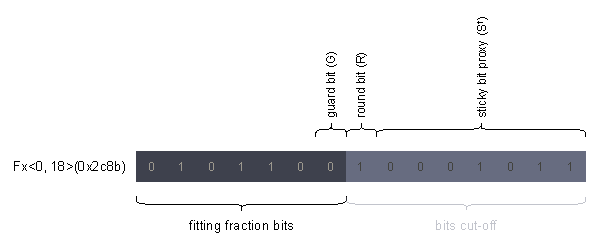
\includegraphics[width=\textwidth]{figures/bits-fraction.drawio.pdf}
    \caption{Bit-string layout of the fraction before rounding, with (G, R, S) bits highlighted}
    \label{fig:fraction_before_rounding}
    \end{center}
\end{figure}


\section{In-depth: division of fractions}\label{Approximated_Algorithms}
In this section, we will address the different existing solutions to compute the fractional part division.
% \footnote{explicit base 2 notation}
\begin{equation}
\frac{(1.f_1)}{(1.f_2)}
\end{equation}

When implemented in hardware, different non-negligible trade-offs come into play.

There are three main families of division algorithms \cite{muller_hardware_2010}. 

\begin{itemize}

\item Digit-recurrence (DR) algorithms, such as the family of SRT algorithms named after Sweeney, Robertson, and Tocher, %[344, 408]
generalize the paper-and-pencil algorithm. They produce one digit of the result at each iteration. Each iteration performs three tasks (just like the pencil-and-paper method): (i) determine the next quotient digit, (ii) multiply it by the divider, and (iii) subtract it from the current partial remainder to obtain a partial remainder for the next iteration.
In binary, there are only two choices of quotient digits, 0 or 1; therefore, the iteration reduces to one subtraction, one test, and one shift. 
A binary digit-recurrence algorithm can therefore be implemented on any processor as soon as it is able to perform integer addition.

One important thing about digit-recurrence algorithms is that they are exact. Starting from fixed-point numbers $X$ and $D$, they compute at iteration $i$ an $i$-digit quotient $Q_i$ and a remainder $R_i$ such that the identity $X = DQ_i + R_i$ holds.
For floating-point purposes, this means that all the information needed for rounding the result is held in the pair $(R_i, Q_i)$. In practice we limit the number of digits for the division result to $p$, introducing an approximation.
%In practice, to round to precision $p$, one needs $p$ iterations to compute $Q_p$, then possibly a final addition on $Q_p$ depending on a test on $R_p$.


\item Polynomial approximation can also be used to evaluate $1/x$ to the required accuracy. %[430].
Note that, mathematically speaking, functional iterations evaluate a polynomial in the initial approximation error. % [88].

\item Functional iteration algorithms generalize the Newton-Raphson iteration for approximating the function $1/x$. They make sense mostly on processors having a hardware multiplier. The number of iterations is much less than in digit-recurrence algorithms ($\mathcal{O}(\log p)$ versus $\mathcal{O}(p)$), but each iteration involves multiplications and is, therefore, more expensive. These latter two methods may be combined.
\end{itemize}

\subsection{Approximated reciprocal}

In order to compute an approximated reciprocate, we can think of exploiting the Taylor series technique\footnote{Wikipedia. 2022. "Taylor series." Wikimedia Foundation. Last modified October 4, 2022. https://en.wikipedia.org/wiki/Taylor\_series.} around $ 0.75 = mean([0.5, 1))$.


However, this approach presents some inconveniences:
\begin{itemize}
\item it requires $6$ fixed-point products\footnote{$3$ due to 3rd-order term $x*x*x*3.1604\dots$ + $2$ + $1$},
\item it is accurate just around the point where the series is expanded, as shown in figure \ref{fig:relative_error_00001}.
\end{itemize}
A way to circumvent the latter issue comes from employing the Chebyshev polynomials. They are used to provide the best approximation not only around a given point but across an interval.
As a trade-off, the better control over the accuracy across this interval comes at the cost of increased computational complexity, compared to the plain Taylor expansion.


Applying the third-order Chebyshev polynomials \cite{Hale2015}formula to $1/x$ across the interval $(0.5, 1)$ we obtain
\begin{equation}\label{equ:3rd_order_Chebyshev_polynomial_equation}
f_{cp_3} = 5.65685 - 11.75737x + 10.64818x^2 - 3.54939 x^3 + \mathcal{O}(x^4)
\end{equation}
which, from the visual comparison with other approximations (figure \ref{fig:relative_error_00001}) seems to return a better approximation of the $1/x$ function across the interval. However, similarly to the Taylor expansion, it still suffers from the long chain of fixed-point products.

A different idea comes from \cite{drom}, with a fast technique for approximated reciprocate computation. In particular, this approach offers three main advantages: (i) no dividers, except division by powers of $2$; (ii) minimal amount of multipliers; (iii) integer arithmetic only.


The following routine is indeed hardware friendly, as it employs just two integer multiplications and a bit shift.

\begin{verbatim}
def reciprocal(a):
    b = 1.466 - a
    c = a * b
    d = 1.0012 - c
    e = d * b
    out = e * 4
    return out
\end{verbatim}


\begin{figure}
    \centering
    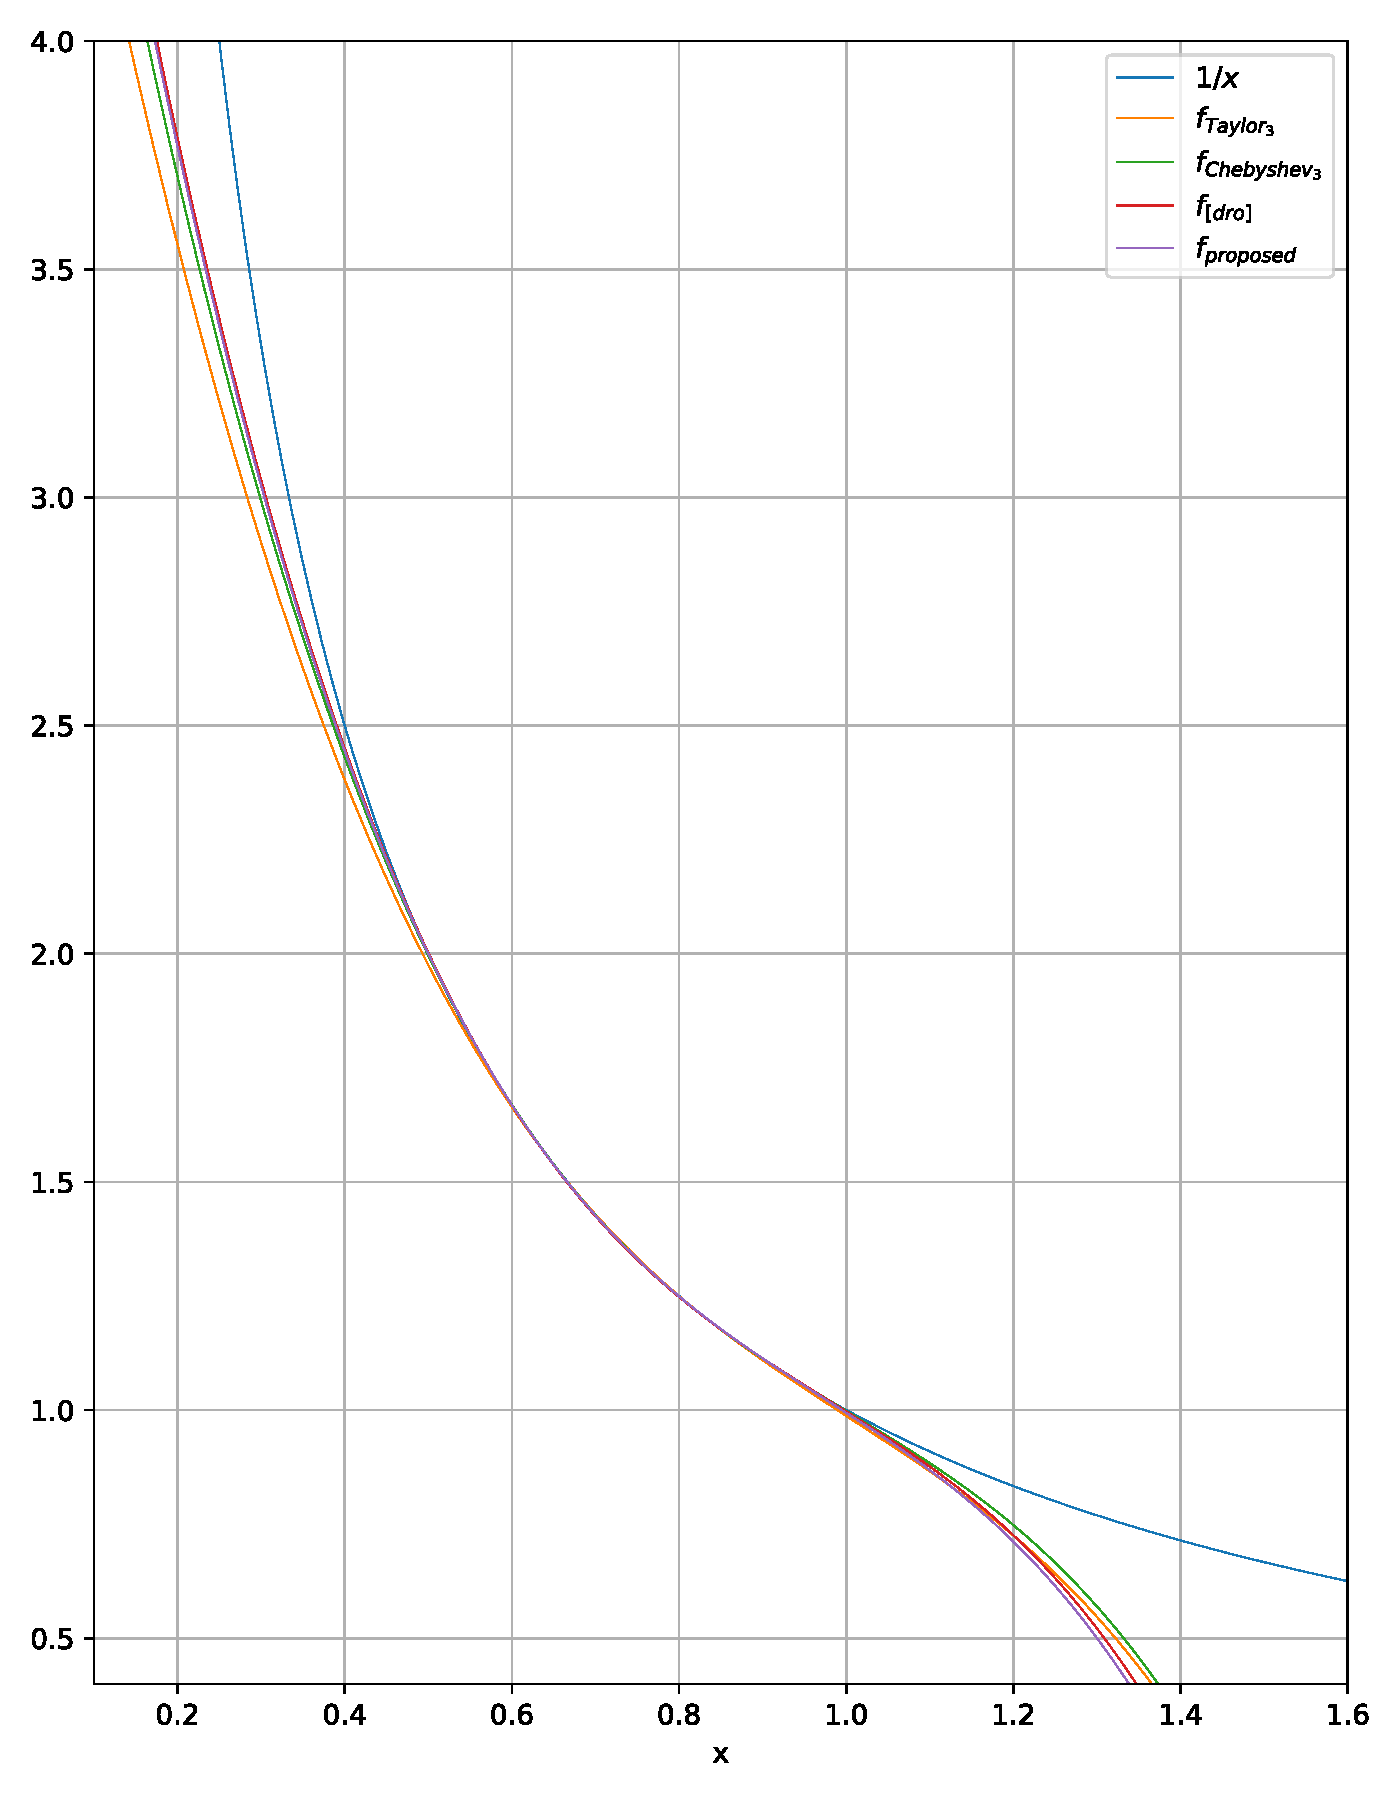
\includegraphics[width=0.75\textwidth]{figures/reciprocate_real_vs_taylor_vs_drom.pdf}
    \caption{Comparison of $1/x$ vs \cite{drom} vs 3rd order Taylor polynomial vs 3rd order Chebyshev polynomial vs proposed solution (i.e. optimized \cite{drom})}
    \label{fig:0203012875432985734}
\end{figure}

\begin{figure}
    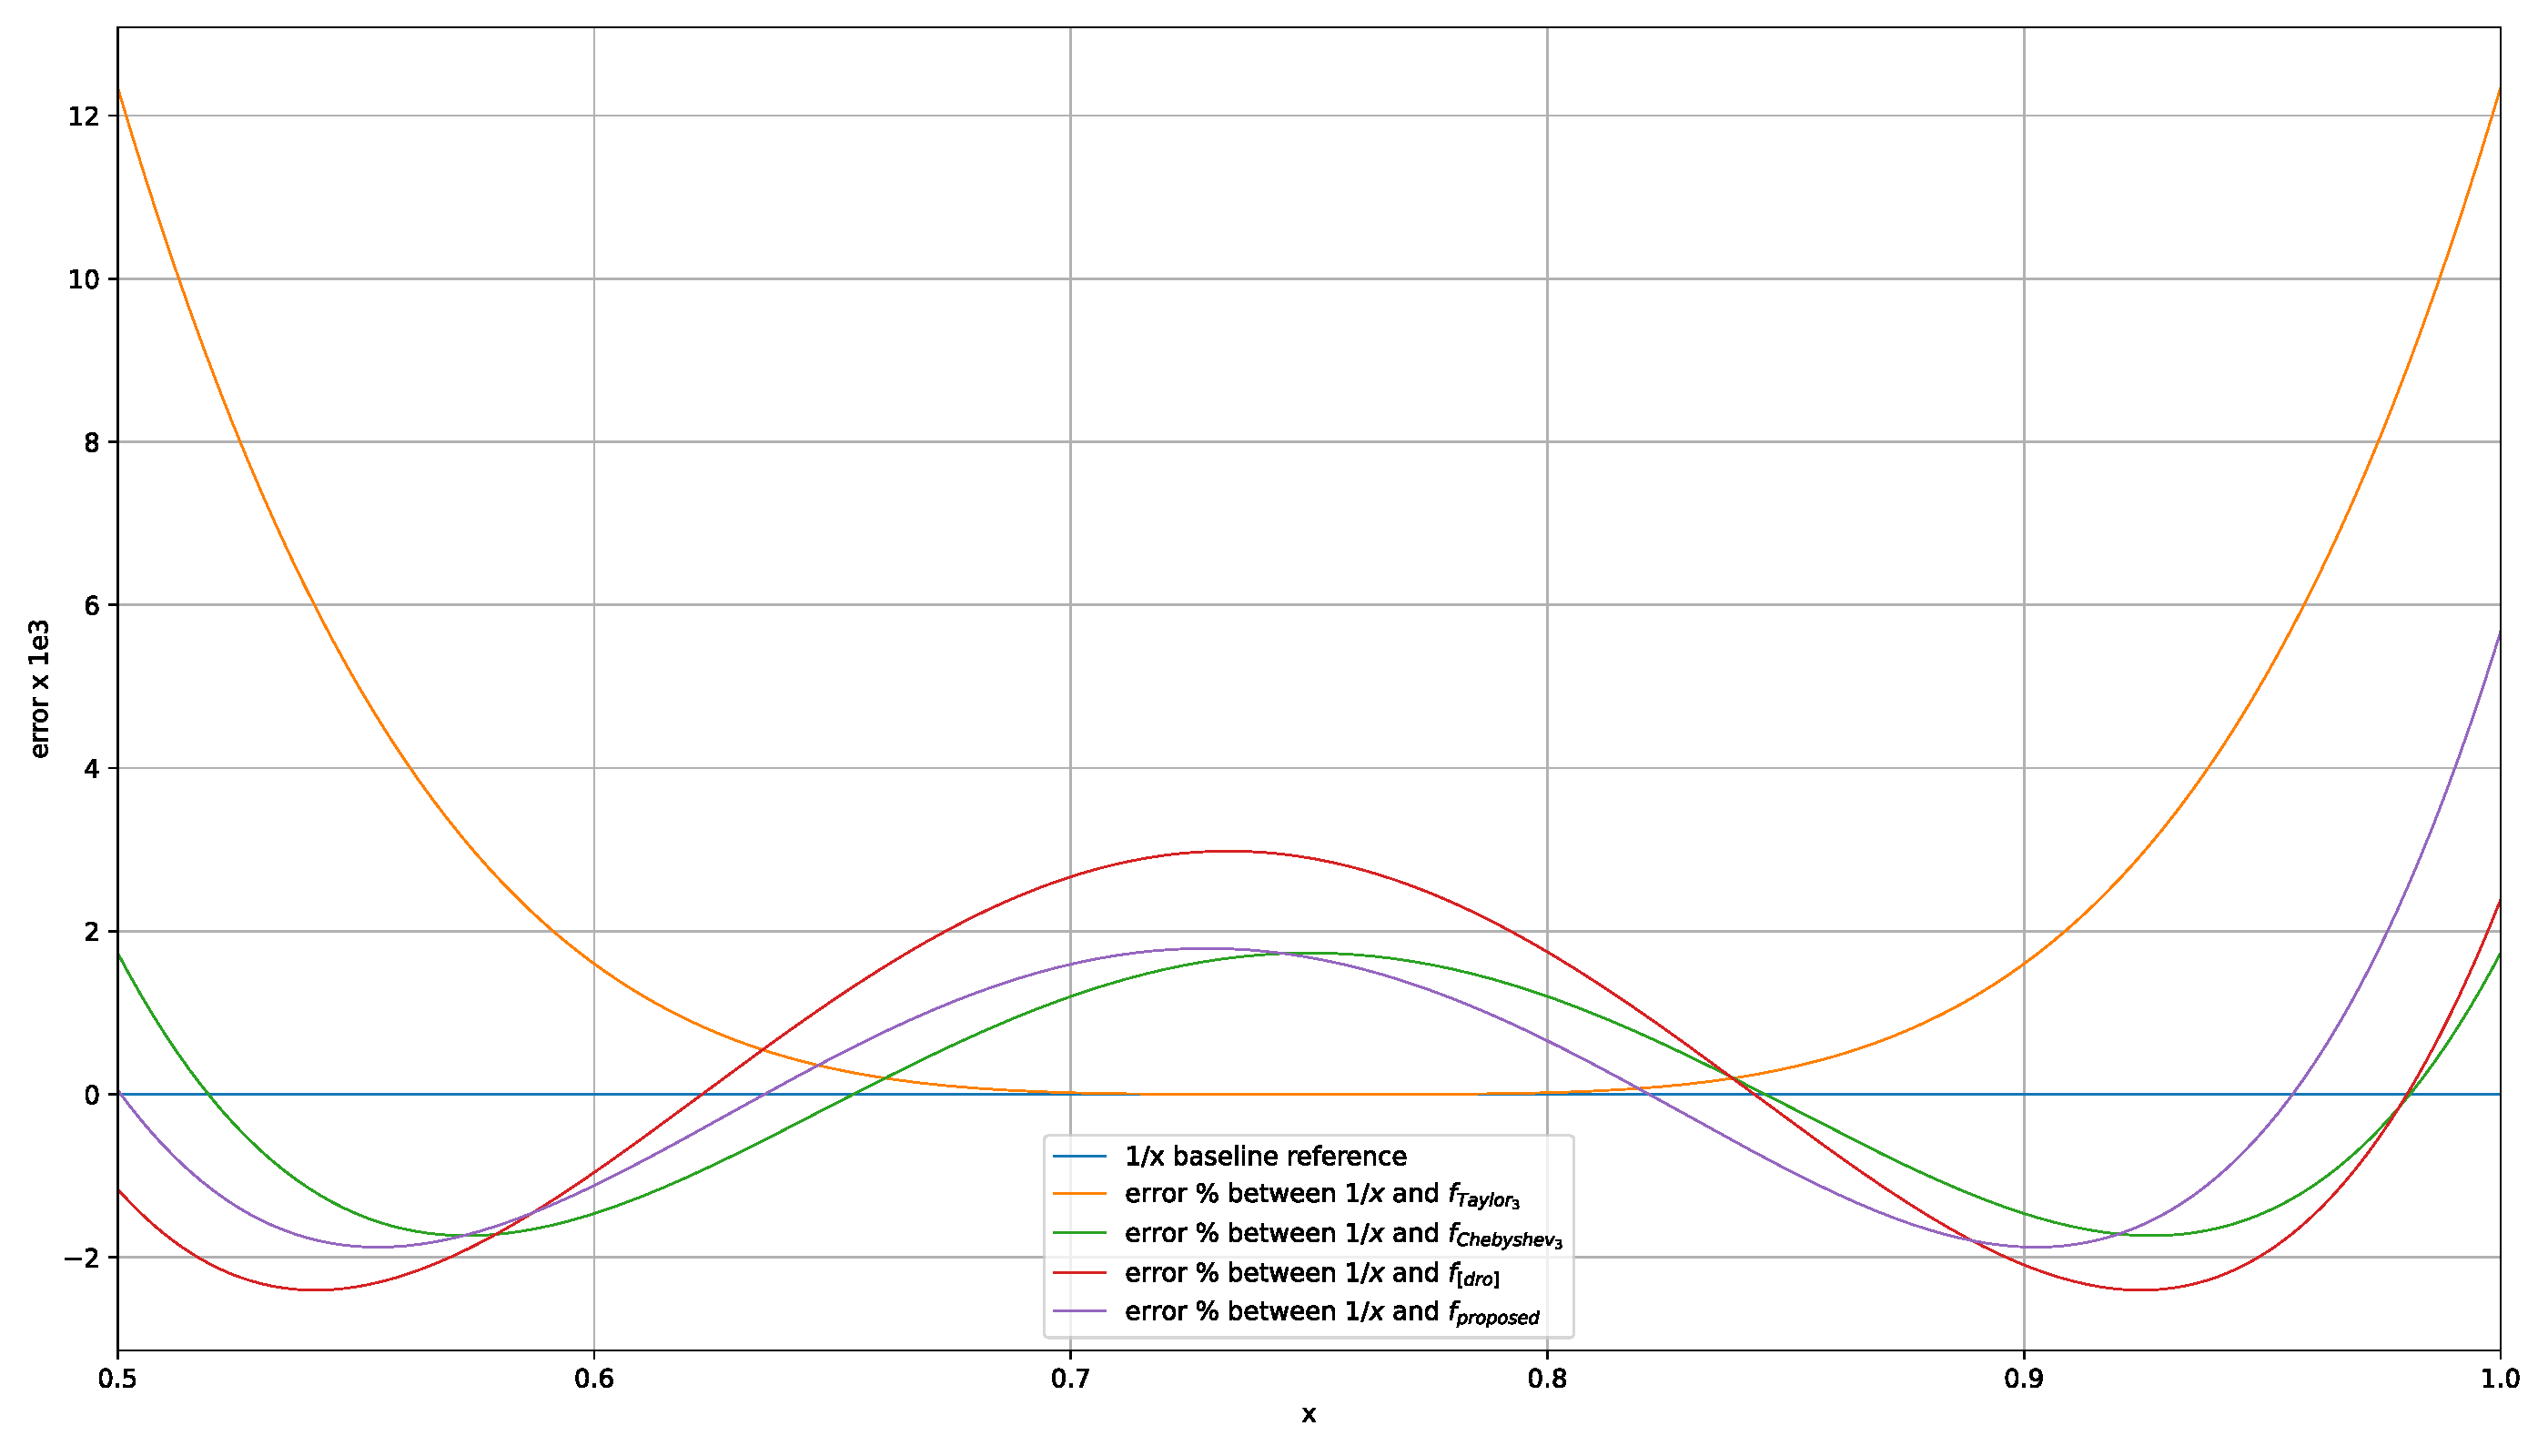
\includegraphics[width=1\textwidth]{figures/reciprocate_real_vs_taylor_vs_drom_error.pdf}\caption{Relative error against reference $1/x$}\label{fig:relative_error_00001}
\end{figure}
\begin{figure}
    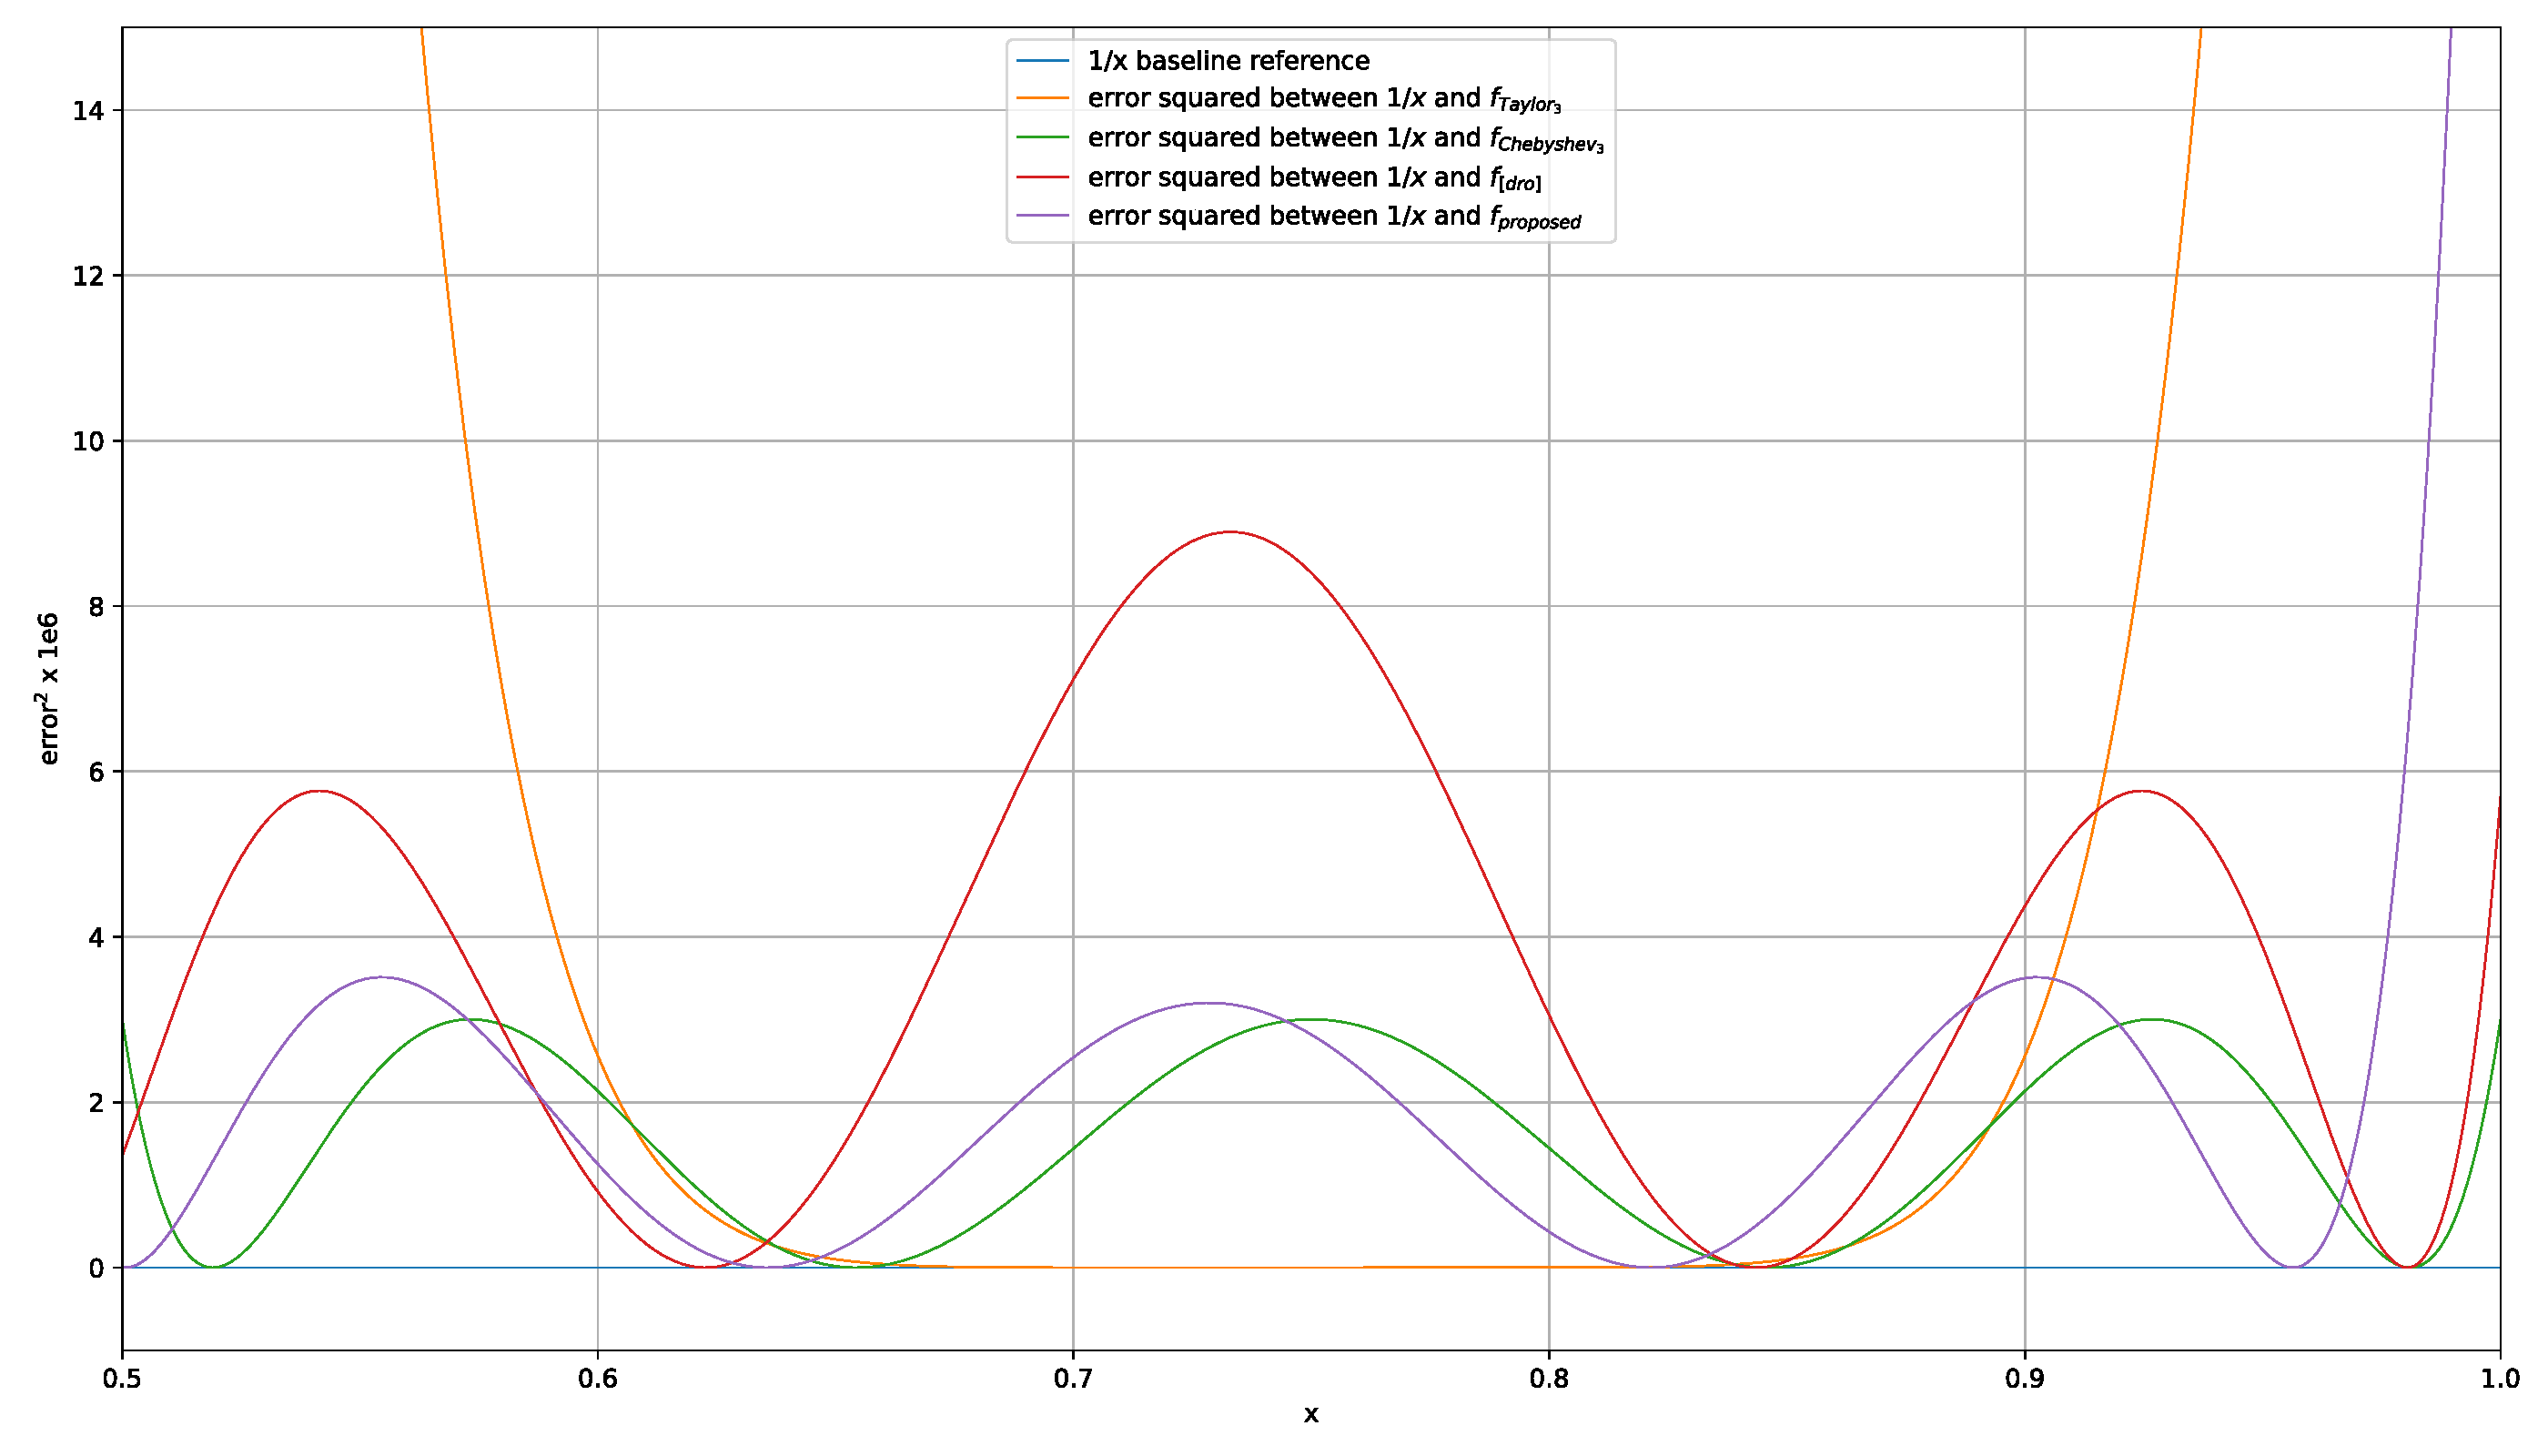
\includegraphics[width=1\textwidth]{figures/reciprocate_real_vs_taylor_vs_drom_error_squared.pdf} 
    \caption{Squared relative error against reference $1/x$}
    \label{fig:020301280980435232835} 
\end{figure} 

If we expand the routine into a  third-order polynomial (\ref{equ:expanded_drom_modified_polynomial}, \ref{equ:expanded_drom_0000}) similar to the previous ones, we can see that this is a modified Chebyshev polynomial with the highest grade coefficient rounded to the closest power of two -- $4$ in this case.
This constraint on the highest grade coefficient reduces the long-chained multiplication required by the original Chebyshev polynomial approximation (\ref{equ:3rd_order_Chebyshev_polynomial_equation}), with a slight degradation in accuracy.
\begin{equation}\label{equ:expanded_drom_modified_polynomial}
\begin{aligned}
f(a, k_1, k_2) &= 4 \cdot e = 4 \cdot d \cdot b = \\
&= 4 \cdot (k_2 - c) \cdot (k_1 - a) = \\
&= 4 \cdot (k_2 - a \cdot b) \cdot (k_1 - a) = \\
&= 4 \cdot [k_2 - a \cdot (k_1 - a)] \cdot (k_1 - a) = \\
&= 4 \cdot (k_2 - k_1 a + a^2) \cdot (k_1 - a) = \\
&= 4 \cdot (k_1 k_2 - k_2 a - k_1^2 a + 2 k_1 a^2 - a^3) = \\
&= 4 k_1 k_2 - 4(k_1^2 + k_2) a + 8 k_1 a^2 - 4 a^3
\end{aligned}
\end{equation}

Let $e^2$ be an error function to compare the accuracy of the different methods presented before. The function $e^2$ corresponds to the underlying area below the curves in Figure \ref{fig:020301280980435232835}. The value $rerr$ indicates the relative error between the real and the approximated function\footnote{$|rerr|$ would have given a comparably meaningful Function of Merit, however, the function must be differentiable in the entire domain, hence $rerr^2$}.


\begin{figure}
    \centering
    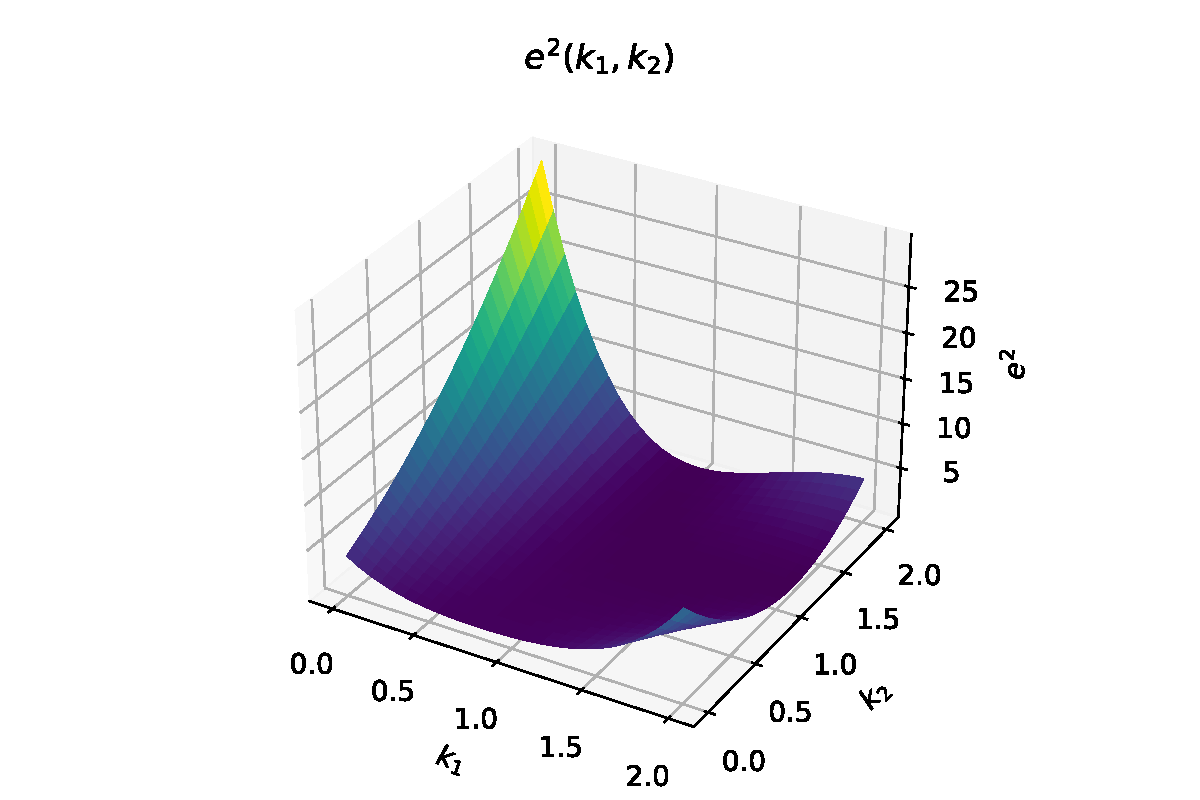
\includegraphics[
        %scale=1
        width=1\linewidth,]{figures/3d_plot_error_squared.pdf}
    \caption{\\$e^2(k_1, k_2)$}
    \label{fig:errorsquared3dplot}
\end{figure}
    
Let $f_{[dro]}$ be the Chebyshev polynomial defined using the coefficients as in \cite{drom}:

\begin{equation}\label{equ:expanded_drom_0000}
\begin{aligned}
f_{[dro]}(a) &= f(a, k_1=1.466, k_2=1.0012) = \\
&= 5.8710368 - 12.601424 a + 11.728 a^2 - 4 a^3
\end{aligned}
\end{equation}

 \begin{equation}\label{equ:equation_e_squared_k1k2}
            \begin{aligned}
            e^2(k_1, k_2) &=  \int_{1/2}^{1} rerr^2(x, k_1, k_2)\ dx = \\
            &= \int_{1/2}^{1} \left( \frac{f(x, k_1, k_2) - 1/x}{1/x} \right)^2 dx = \\
            &= \int_{1/2}^{1} \left( \frac{k_1 k_2 - 4(k_1^2 + k_2) x + 8 k_1 x^2 - 4 x^3 - 1/x}{1/x} \right)^2 dx = \\
            &= \frac{31 k_{1}^{4}}{10} - \frac{15 k_{1}^{3} k_{2}}{2} - \frac{21 k_{1}^{3}}{2} + \frac{14 k_{1}^{2} k_{2}^{2}}{3} + \frac{93 k_{1}^{2} k_{2}}{5} + \\ 
            &+ \frac{1339 k_{1}^{2}}{84} - \frac{15 k_{1} k_{2}^{2}}{2} - \frac{75 k_{1} k_{2}}{4} - \frac{375 k_{1}}{32} + \frac{31 k_{2}^{2}}{10} + \\ 
            &+ \frac{577 k_{2}}{84} + \frac{5507}{1440}
            \end{aligned}
        \end{equation}
        
We may want to know which are the optimal $k_1$ and $k_2$ such that:
\begin{equation}\label{equ:opt_k1_k2_eq}
(k_{1_{opt}}, k_{2_{opt}}): \min\{e^2(k_1, k_2)\}
\end{equation} 

For that the following system of equations (\ref{equ:opt_k1_k2_eq}) must be solved:
\begin{equation}\label{equ:opt_k1_k2_eq_partial}
\begin{cases}
\dfrac{\partial}{\partial k_1} e^2(k_1, k_2) = 0 \\
\dfrac{\partial}{\partial k_2} e^2(k_1, k_2) = 0
\end{cases}
\end{equation} 
\iffalse
$$
\begin{cases}
k_{1_{opt}} = 1.4567844114901045 \\
k_{2_{opt}} = 1.0009290026616422
\end{cases}
$$
\fi
which gives $(k_{1_{opt}} = 1.4567844114901045,\ k_{2_{opt}} = 1.0009290026616422)$, yielding a $36.4\%$ improvement over \cite{drom}'s $e^2$. Figure \ref{fig:are_barplot} shows a comparison of the relative accuracy of the above-mentioned functions and techniques compared to $1/x$.

\begin{figure}
    \begin{center}
    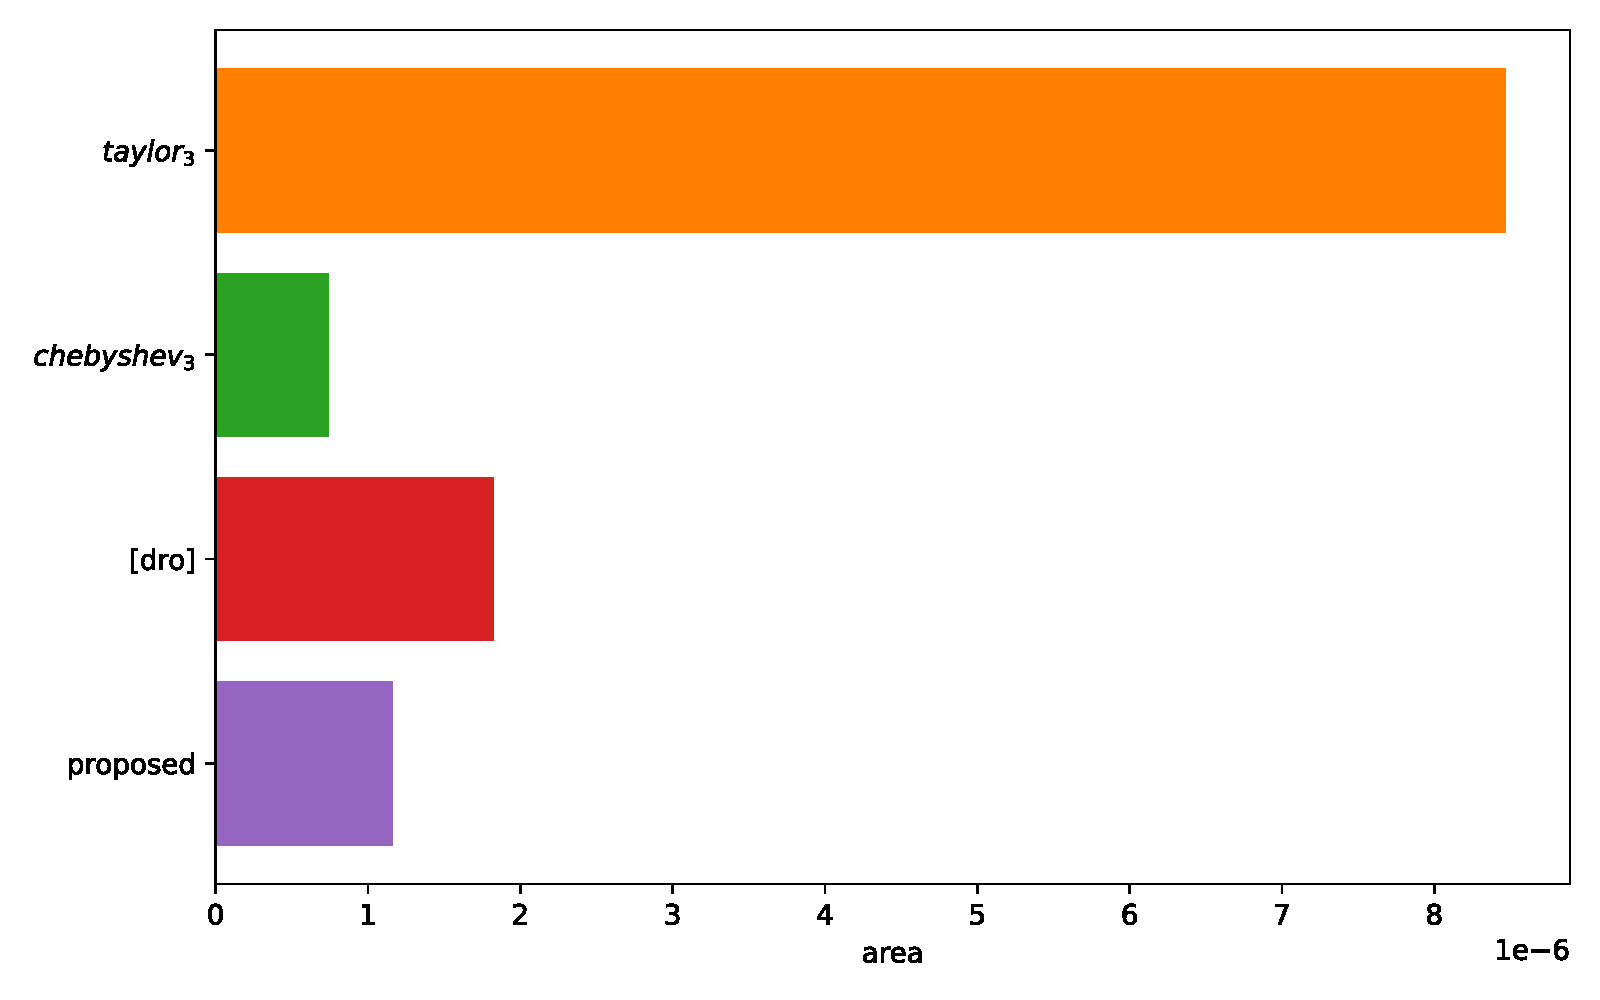
\includegraphics[width=0.4\textwidth]{figures/barplot_area_error.pdf}
    \caption{Barplot error area. $taylor_3$ vs $chebyshev_3$ vs \cite{drom} vs proposed}
    \label{fig:are_barplot}
    \end{center}
\end{figure}


Using the optimal $k_1$ and $k_2$ coefficients -- i.e. (i) Chebyshev-like polynomial, and (ii) highest grade coefficient being a power of $2$\footnote{so that the bit shift trick can be performed, as opposed to yet another multiplication} -- we can now use the following algorithm to perform the approximated reciprocal:

\begin{lstlisting}[label=alg:reciprocal_approx_modified_drom]
def reciprocal(a):
    b = k1_opt - a
    c = a * b
    d = k2_opt - c
    e = d * b
    out = e << 2
    return out
\end{lstlisting}

The numerical bounds of the result of each step in the algorithm can be determined so that we can set the correct fixed-point representation, allocating enough bits.

The input is a mantissa, hence contained in $[1, 2)$: in order to fit in the range required by the algorithm, that is $[0.5, 1)$, we divide by $2$, or, we just operate a one-bit right shift. Similarly, a division by $2$ is required when the algorithm terminates to restore the pre-normalization value.


Figure \ref{fig:reciprocal_unsigned_workflow} shows the flow of the procedure. 



\begin{itemize}
    \item \texttt{a} $\in [0.5, 1) \equiv A $ \dotfill \texttt{Fx<0, F>}
    \item \texttt{b} $\in (0.45702824, 0.95702824] $ \dotfill \texttt{Fx<0, F>}
    \item \texttt{c} $\in (0.45702824, 0.5307166278550605) $ \dotfill \texttt{Fx<0, 2F>}
    \item \texttt{d} $\in (0.47022002214493963, 0.54390841) $ \dotfill \texttt{Fx<0, 2F>}
    \item \texttt{e} $\in (0.24858150334349846, 0.4999731144222473) $ \dotfill \texttt{Fx<0, 3F>}
    \item \texttt{out} $\in (0.9943260133739938, 1.9998924576889892) $ \dotfill \texttt{Fx<1, 3F>}
\end{itemize}



    

\begin{figure}
    \centering
    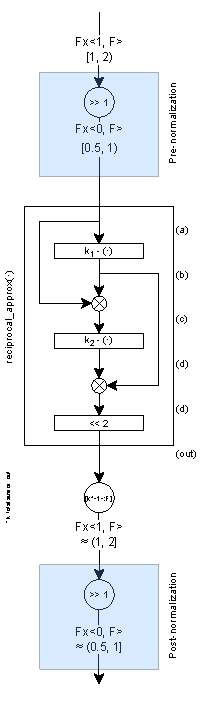
\includegraphics[width=0.28\textwidth]{figures/reciprocal_unsigned.drawio.pdf}
    \caption{Reciprocal unsigned workflow}
    \label{fig:reciprocal_unsigned_workflow}
\end{figure}

\subsection{Ahead-of-time reciprocal}\label{aot_reciprocal_lut_technique}

The previous solution presents a reduced result's precision (due to the approximated reciprocate) with the benefit of a reduction in required hardware resources.
Another solution called \textit{Ahead Of Time} computation of the reciprocate, helps with the accuracy drop seen before: the core idea is that instead of computing the reciprocate on-demand, we store the reciprocates inside a look-up table (as in \cite{PACoGen}). Such a look-up table takes $N$ bits representing the $N$ most significant bits of the fraction as input and will output the $M$ most significant bits of the reciprocate of the input.

\begin{figure}[h!]
    \begin{center}
    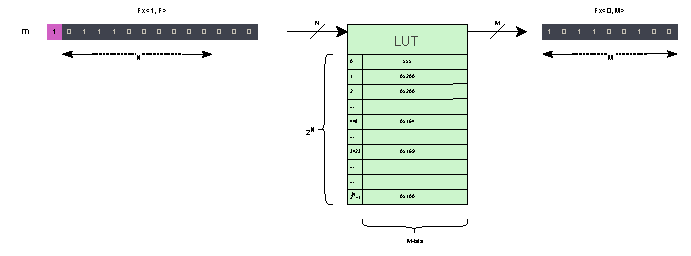
\includegraphics[width=1\textwidth]{figures/lut.drawio.pdf}
    \caption{Look Up Table example, taking P$\langle 16,1 \rangle(0x71c0)$'s mantissa as input}
    \label{fig:lut_drawio_example}
    \end{center}
\end{figure}

Concerning the same posit, $P\langle 16,1 \rangle(0x71c0)$, figure \ref{fig:lut_drawio_example} gives an example of the mechanism: i) the fraction field is adjusted to $N$ bits (this can be either a bit-expansion or a bit-compression); ii) the value represented by those bits is used to index the element in the look-up table resulting in the $M$ most significant bits of the reciprocate of the full input mantissa.

The lookup table gives another degree of freedom: $N$ and $M$ can be set independently from the posit size to account for the trade-off between resource utilization and required accuracy for the reciprocate.


\subsection{Newton-Raphson}\label{Newton_Raphson}


In numerical analysis, the Newton–Raphson method \cite{Hale2015_a} is a root-finding algorithm which produces successively better approximations of the roots of a real-valued function. The most basic version starts with a single-variable function $f$ defined for a real variable $x$, the function's derivative $f'$, and an initial guess $x_0$ for a root of $f$.
If the function satisfies sufficient assumptions and the initial guess is close, then the algorithm is guaranteed to converge to a root of $f$. The iterative scheme for the algorithm is shown in \eqref{equ:newon_raphson_generalized_equation}:

\begin{equation}\label{equ:newon_raphson_generalized_equation}
x_{n+1} = x_n - \frac{f(x_n)}{f'(x_n)}
\end{equation}

This technique can be exploited to solve the problem of interest by noticing that if we consider a function whose root is such that $x = 1/k$, e.g.
\begin{equation}
f(x) = \frac{1}{x} - k
\end{equation}
with derivative
$$
f'(x) = -\frac{1}{x^2}
$$
where $n$ is the number whose reciprocate we are after and $x$ the reciprocate itself, the Newton Raphson method gives
\begin{equation}
\begin{aligned}
x_{n+1} &= x_n - \frac{f(x_n)}{f'(x_n)} = \\
& = x_n - \frac{\dfrac{1}{x_n} - k}{-\dfrac{1}{x_n^2}} = \\
& = x_n\ (2 - k \cdot x_n)
\end{aligned}
\end{equation}
which yields a valid approximation so long as the initial guess $x_0 \in (0, 2/k)$, to not make the iteration diverge.


 % uncomment if you want part I
\chapter{Implementing a multi-architecture posit library}


\section{Overview of existing posit libraries}

In this chapter we will focus on presenting and analyzing posit libraries, including the one created and maintained by us. We will consider the \texttt{C++} based libraries.
Having software support for a new type is of utmost importance. A software library supporting posits should have the following properties:
\begin{enumerate}
    \item Can hot-swap the binary32 \textit{float} type without changing much code
    \item Supports a wide range of posit configurations, typically defined at compile time
    \item Avoids to implement posit operations directly using a $1:1$ hardware correspondence in software 
\end{enumerate}

Property 1) is typically obtained by having a posit type that overloads most of the basic arithmetic operators (e.g. +,-,*,/ and their variations). Furthermore, machine learning and linear algebra applications make extensive use of numerical \textit{traits} to calibrate the algorithms. Therefore, a good posit library should also implement them to fulfil property 1). 

Property 2) can be achieved by templetization of the code. In particular, we should have, at minimum, $2$ template parameters: one for the number of bits $nbits$ and one for the number of exponent bits $esbits$. We will see  in the following sections that we can achieve more degrees of freedom with more templates parameter.

Property 3) is strictly related to the computing performance of the library. In this phase, we pretend not to have any hardware support for the library. Therefore, software emulation of posits occurs. This can be done either by exactly reproducing what a posit-enabled hardware would perform for the various operations or relying on a back-end format for computations. Such a format should have complete hardware support to handle computations efficiently. Property 3) can also be fulfilled with pre-computation of posit operations, thus creating software look-up tables that can be addressed to obtain result of operations without actually computing them.


\subsection{SoftPosit}

SoftPosit \cite{softposit} is one of the first open-source posit libraries appeared. The core is \textit{C} based, but the library offers interfaces for C++, Python and Julia. 

While the core C library obviously does not offer operator overloading, the included C++ API interface offers such feature. However, there is no support for numerical traits inside the C++ interface. Therefore the property 1) we expressed before is not completely satisfied by this library.

SoftPosit offers the following posit configurations:
\begin{itemize}
    \item \posit{32}{2}
    \item \posit{16}{1}
    \item \posit{8}{0}
\end{itemize}

\lstinputlisting[caption={Example of use of SoftPosit with a \posit{8}{0}},label={lst:softPosit8}]{snippets/softposit8example.c}

The posit type is represented by a C \texttt{struct} called  \texttt{posit<bits>\_t}, where \texttt{<bits>} is the number of posit bits. Posit values are stored as signed integers. The size of the integer depends on the size of the posit considered:

\begin{itemize}
    \item \posit{32}{2}: \texttt{posit32\_t} stored in a \texttt{int32\_t}
    \item \posit{16}{1}: \texttt{posit16\_t} stored in a \texttt{int16\_t}
    \item \posit{8}{0} : \texttt{posit8\_t}  stored in a \texttt{int8\_t}
\end{itemize}

These configurations are statically typed inside the library so there is no flexible way to express a desired configuration for the posit at compile time (except for deeply modifying the library). Therefore, property 2) does not hold in this case.

Looking at the internals of SoftPosit we can see that each operation between posit is represented by a function in the format \texttt{p<bits>\_<op>}, where \texttt{<bits>} is the number of posit bits and \texttt{<op>} is the name of the operation (e.g. 'add').

Listing \ref{lst:softPosit8} and \ref{lst:softPosit16} show an example of the C API used to sum two \posit{8}{0} or two \posit{16}{1}.



\lstinputlisting[caption={Example of use of SoftPosit with a \posit{16}{0}},label={lst:softPosit16}]{snippets/softposit16example.c}


Posit operations are implemented following the hypothetical hardware implementation of a posit processing core; indeed, the evaluation of operations not only involves the decoding of the posit to its fields, but also manipulation of such fields to perform the operations. Due to this choice also the property 3) cannot hold.

\section{The cppPosit core}\label{sec:cppPositCore}

The cppPosit library revolves around the idea of a highly template-ized type that can bet dropped in place of the C++ native \texttt{float} in any application. 

The main class of the library is the \textit{posit} class, as reported in Listing \ref{lst:positClassCore}.  

\lstinputlisting[caption={Posit class core},label={lst:positClassCore}]{snippets/positclass.cpp}

The template meaning is the following:
\begin{itemize}
    \item \texttt{class T}: storage (or holder) type for the posit. Typically aligned to power of 2. For example: \texttt{int8\_t}, \texttt{int16\_t}, \texttt{int32\_t}
    \item \texttt{totalbits}, \texttt{esbits}: respectively, the posit parameters for $nbits$ and $esbits$ as shown in previous sections.
    \item \texttt{FT}: backend type for the posit: can be a fixed-point or a floating-point backend (more on this in the following section).
    \item \texttt{positSpec}: specific class to represent a configuration for posit with \textit{Infinity} or \textit{Not a Real} for the North point of the posit ring.
\end{itemize}

The template also enforces some controls over its arguments. Indeed, the value \texttt{totalbits} needs to be lower or equal than the size of the storage type \texttt{T}. Furthermore, the backend type \texttt{FT} needs to be big enough to contain the dynamic range of the represented posit.


\subsection{Operation levels}

When considering posits, we can classify its operations in 4 different levels:

\begin{itemize}
    \item $\mathcal{L}_1$: level-one operations are implemented with a direct manipulation of the posit bit representation (e.g. all the fast-approximated operations seen in previous chapter lie in this level).
    \item $\mathcal{L}_2$: level-two operations need the decoding of the posit into its fields (sign, regime, exponent and fraction). Typically these operations are used to obtain one of the posit fields to manipulate it (e.g. increasing the regime when doubling a posit with more than 0 exponent bits).
    \item $\mathcal{L}_3$: level-three operations require to decode the posit as in $\mathcal{L}_2$ and build the joint regime-exponent value. This operations are required to transform a posit into a format in the FIR space as seen in Section \ref{sec:fir}. A common use of these operations is indeed the conversion of a posit to another floating point format (e.g. IEEE binary32).
    \item $\mathcal{L}_4$: level-four operations require the transformation of a posit to its backend,to compute operators like $+,*,-,/$ and others.
\end{itemize}

\subsection{One frontend, different backends}

As described in the previous Subsection, one of the template arguments of the posit class is the backend type, used to control the actual implementation of posit operations in $\mathcal{L}_4$.

We have 3 different class of backends implemented in cppPosit:
\begin{itemize}
    \item Integral backend (\texttt{Unpacked}): the posit backend is actually the integer where it is stored and the computations are performed emulating an ideal posit processing unit hardware (this is completely similar to the softposit approach).
    \item Floating point backend (\texttt{BackendFloat}): posit computation in $\mathcal{L}_4$ are not performed on the posit representation. Instead, the posit is transformed to a floating point number (e.g. binary32 or binary64) through the FIR representation and then computation are performed using native hardware support for such formats. At the end, the result is converted back to posit. 
    \item Fixed point backend (\texttt{BackendFixed}): this backend exploits fixed-point arithmetic to perform posit computation. Similar to the floating point backend, posit numbers are converted to fixed-point before computations and are reconstructed from fixed-point result after the operations.
\end{itemize}

A particular note on the \texttt{BackendFixed} backend must be outlined: in the library we identify the fixed point backend with a \texttt{FixedTrait} trait template, that contains the number of bits of the fixed point integer to be used. We enforce that this amount of bits is enough to contain the posit dynamic. 

Given a fixed point $Fx$on $L$ bits, we know that the maximum representable value is $2^{L/2 - 1}$ (rounded upwards considering the additional $L/2$ fractional bits). On the other hand, the maximum posit value is $\text{maxposit} = useed^{(nbits - 2)}$. We then need to impose that $max(Fx) \geq maxposit$: 

\begin{equation}
    2^{\frac{L}{2} - 1} \geq  useed^{(nbits - 2)}
\end{equation}

\begin{equation}
    2^{\frac{L}{2} - 1} \geq 2^{2^{esbits} \cdot (nbits - 2)}
\end{equation}

\begin{equation}
    \frac{L}{2} \geq 2^{esbits} \cdot (nbits - 2) + 1
\end{equation}

\begin{equation}
    L \geq 2^{esbits + 1} \cdot (nbits - 2) + 2
\end{equation}

Table \ref{tab:fixedPointToPositSize} summarizes the requirements for the fixed point backend for different posit configurations.

\begin{table}[]
\centering
\caption{Summary of required Fixed point bits for different posit configurations}
\label{tab:fixedPointToPositSize}
\begin{tabular}{lllll}

bits & esbits & useed & min(L) & Fixed point bits \\ \hline
8    & 0      & 2     & 14     & 16               \\
8    & 1      & 4     & 26     & 32               \\
8    & 2      & 16    & 50     & 64               \\
16   & 0      & 2     & 30     & 32               \\
16   & 1      & 4     & 58     & 64               \\
16   & 2      & 16    & 114    & 128              \\ \hline
\end{tabular}
\end{table}

Listing \ref{lst:positDefinitionCppPosit} shows some examples of posit definitions using different backends. A particular definition is the last one. Indeed, we can use more than the needed bits for the fixed point as a posit backend. Doing so, we can reach the point where the fixed point is big enough to hold accumulation of posit values, thus obtaining an accumulator similar to a \textit{quire}.

Having this possibility means that we can implement \textit{multiply-add} operations where consecutive accumulation of posit-posit multiplication are represented on a fixed point big enough not to introduce any rounding during all the process.  

\lstinputlisting[caption={Different Posit definition inside cppPosit},label={lst:positDefinitionCppPosit}]{snippets/positDefinitions.cpp}



\subsection{Fast operations with 0 exponent bits}

As we described in previous Section the cppPosit library has a class of operations in $\mathcal{L}_0$ that can be carried out with bit manipulations of the posit bit representation. We already discussed the accuracy impact of these operations in Section \ref{subsec:fastArithOps}. In \cite{coco_et_al_jrtip_2020, coco2020sensors} we also evaluated the impact on the processing time of such operations, in particular the activation functions.

\begin{figure}
    \centering
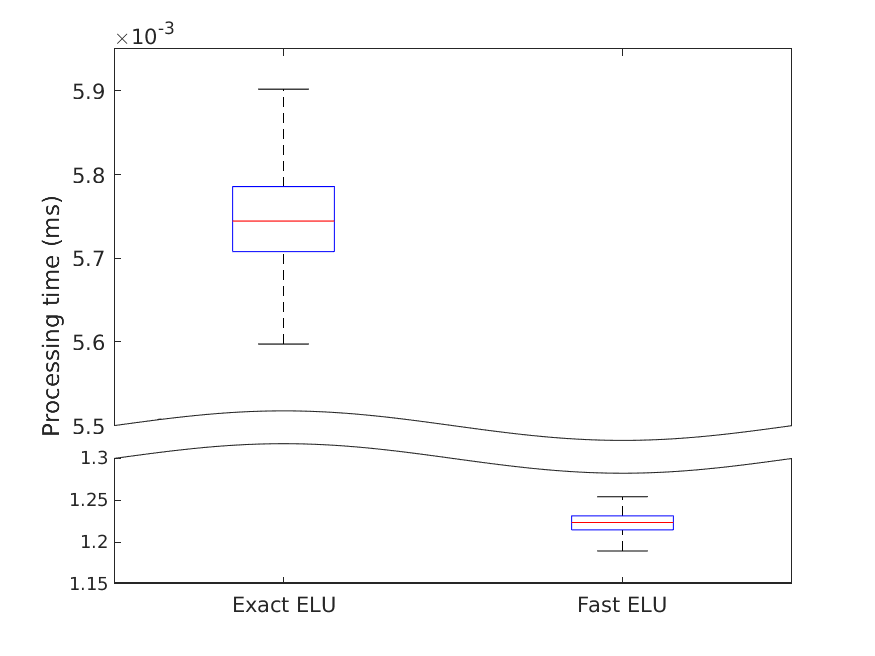
\includegraphics[width=\linewidth]{img/eluTimeComparison.png}
    \caption{Time comparison on the execution of the ELU activation function on the entire \posit{8}{0} domain}
    \label{fig:posit80EluTimeComparison}
\end{figure}

\begin{figure}
    \centering
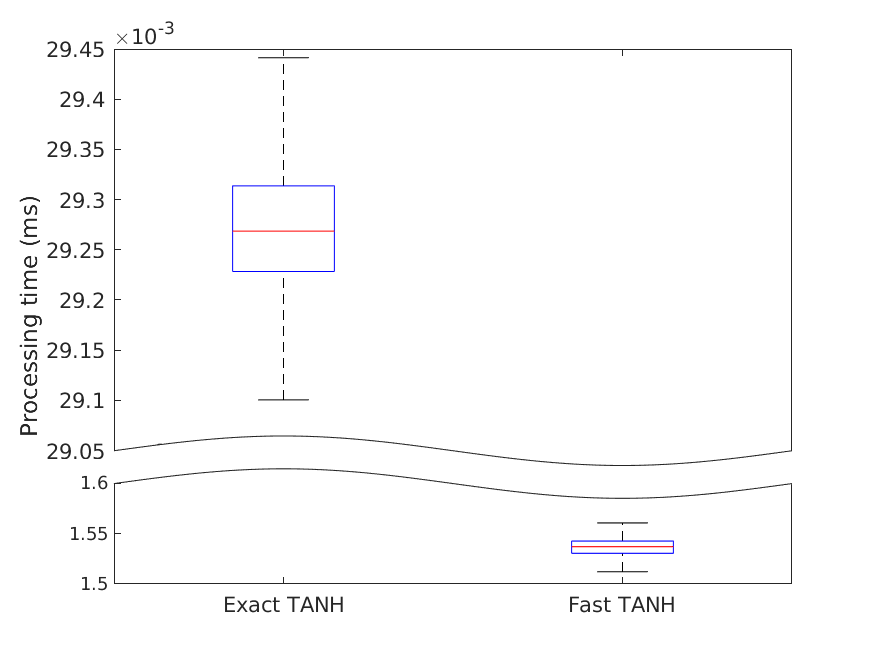
\includegraphics[width=\linewidth]{img/tanhTimeComparison.png}
    \caption{Time comparison on the execution of the TANH activation function on the entire \posit{8}{0} domain}
    \label{fig:posit80ETanhTimeComparison}
\end{figure}

Figures \ref{fig:posit80EluTimeComparison} and \ref{fig:posit80ETanhTimeComparison} show the processing time of the ELU and TANH activation functions evaluated on the entire \posit{8}{0} domain (256 samples). The evaluation was carried out on a 7-th generation \texttt{Intel i7-7560U} processor, running Ubuntu Linux \texttt{18.04}, equipped with \texttt{GCC 8.3}. As we can see from the two plots it is clear how the approximated version outperforms the exact version both in mean value and in variance, being more reliable in the variation of time elapsed for the computation. This stems from the fact that the fast version is evaluated entirely on the ALU, that is traditionally a fixed-latency unit in most of the general purpose processors.

\section{Posit tabulation and logarithmic tabulation}

In the absence of proper hardware support of a Posit Processing Unit (PPU) there still is the need for speeding up the computation. An interesting mean to cope with this problem is the pre-computation of some useful Posit operators in look-up tables. These LUTs become useful when the number of bits is low (e.g. $nbits < 12$).
The core idea is to generate tables for the most important arithmetic operations (addition/subtraction and multiplication/division) for all combination of a given Posit configuration $nbits,esbits$.
Moreover, some interesting functions can be tabulated, in order to speedup their computation, like \textit{logarithm} or \textit{exponentiation}.
Given a $nbits$ bit Posit, with a naive approach, a table will be \[ T \in P^{R \times C} \] where: \[ R=C=2^{nbits}   \]
Depending on the underlying storage type \texttt{T}, each table entry will occupy \texttt{b=sizeof(T)} bits. Typically there will be between $N=8$ and $N=10$ tables for a Posit configuration. This means that the overall space occupation will be \[ S=N \cdot (R \cdot C) \cdot b \]
Table \ref{tab:table_occup} shows different per-table occupation of different Posits configurations. As reported,only Posits with $8$ and $10$ bits have reasonable occupation, considering current generation of CPUs. In fact we can obtain a considerable speedup when one or more tables can be entirely contained inside the cache.

\begin{table}[H]
\centering
\caption{Table occupation for various configurations}
\label{tab:table_occup}
\begin{tabular}{ccc}
\hline \textbf{Total bits (X)}
           & \textbf{Storage type bits (b)}   
           & \textbf{Per-table occupation}
\\ \hline
 \textbf{8} & $8$ & $64$ \textit{KB}\\ \hline
 \textbf{10} & $16$ & $2$ \textit{MB} \\ \hline
 \textbf{12}& $16$ & $32$ \textit{MB} \\ \hline
 \textbf{14}& $16$ & $512$ \textit{MB}\\ \hline
  \textbf{16} & $16$ & $8$ \textit{GB}\\ \hline
\end{tabular}
\end{table}


In order to reduce both LUT size and their number we can exploit some arithmetic properties:
\begin{itemize}
    \item Addition and subtraction are respectively symmetric and anti-symmetric. The two tables can be merged into one and only one half of it is required (above or below the main diagonal).
    \item Multiplication and division can be simplified through logarithm properties. Given $p=x\cdot y$, we can apply $log$ operator on both sides (see \cite{arnold2003interval}), thus obtaining $\log(p) = \log(x\cdot y)$. From logarithm properties this results in \[\log(p) = \log(x)+\log(y)\] Finally, going back with exponentiation we get: \[ p = e^{\log(x)+\log(y)} \] Since tabulation of single operators scales linearly with the Posit size, it is feasible only to store $\exp,\log$ instead of multiplication and division, thus exploiting addition/subtraction LUT for the computation. 
    \item We can compact multiplication tables even more by exploiting the fast inversion (L1) shown in Section \ref{subsec:fastArithOps}. Suppose to have two Posit numbers $x,y$ and their reciprocates, if we want to provide every multiplication or division combination we would build a LUT like in Table \ref{tab:tab_mul_full}. This table would result in 16 entries for only 4 numbers, hence not manageably growing with Posit size. If we apply the L1 inversion and symmetry of negative values, we only need to store the operations for $x\cdot y$ and $x/y$, thus resulting in a LUT size of only 2 elements for the same amount of numbers, as shown in Table \ref{tab:tab_mul_color}.
\end{itemize}

\begin{table}[]
\centering
\caption{All the possible combinations for multiplying and dividing two Posit numbers.}
\label{tab:tab_mul_full}
\begin{tabular}{ccccc}
\hline
\textbf{}     & \textbf{1/x} & \textbf{x} & \textbf{-1/x} & \textbf{-x} \\ \hline
\textbf{1/y}  & 1/xy         & x/y        & -1/xy         & -x/y        \\ \hline
\textbf{y}    & y/x          & xy         & -y/x          & -xy         \\ \hline
\textbf{-1/y} & -1/xy        & -x/y       & 1/xy          & -x/y        \\ \hline
\textbf{-y}   & -y/x         & -xy        & -y/x          & xy          \\ \hline
\end{tabular}
\end{table}

\begin{table}[]
\centering
\caption{All the possible combinations for multiplying and dividing two Posit numbers: all the cells in \textcolor{blue}{blue} correspond to the same LUT entry and the remaining ones correspond to another LUT entry.} \
\label{tab:tab_mul_color}
\begin{tabular}{ccccc}
\hline
\textbf{}     & \textbf{1/x} & \textbf{x} & \textbf{-1/x} & \textbf{-x} \\ \hline
\textbf{1/y}  & \textcolor{blue}{1/xy}         & x/y        & \textcolor{blue}{-1/xy}         & -x/y        \\ \hline
\textbf{y}    & y/x          & \textcolor{blue}{xy}         & -y/x          & \textcolor{blue}{-xy}         \\ \hline
\textbf{-1/y} & \textcolor{blue}{-1/xy}        & -x/y       & \textcolor{blue}{1/xy }         & -x/y        \\ \hline
\textbf{-y}   & -y/x         &\textcolor{blue}{ -xy}        & -y/x          & \textcolor{blue}{xy}          \\ \hline
\end{tabular}
\end{table}

\section{cppPosit in high performance computing environments}
\subsection{ARM Scalable Vector Extension (SVE)}

The ARM Scalable Vector Extension (SVE, \cite{svewhitepaper}) is a vector extension for the ARM AArch64 architecture supported by the ARMv8 instruction set. The main difference between SVE and other single-instruction multiple-data (SIMD) engines (Intel AVX/SSE or ARM NEON) is that it does not specify any width for vector registers, but it provides some constraints for it. The vector register widths must be multiple of $128$ up to $2048$ bits. This approach, called Vector Length Agnostic (VLA), allows us to implement only one vectorized version of our operations, exploiting both auto-vectorization and ARM ACLE (ARM C Language Extensions), without the need to target specific hardware platforms.

\begin{figure}
	\centering    
    \begin{bytefield}[bitwidth=1.5em]{16}
      \colorbitbox{lightcyan}{16}{\scriptsize{Z0 (0..L)}}&\\\\
        \wordbox[]{1}{$\vdots$}\\\\
        \colorbitbox{lightcyan}{16}{\scriptsize{Z31 (0..L)}}&
       
    \end{bytefield}
    \caption{ARM SVE Z Data registers: 32 vector length agnostic register where $L=128\cdot k, k \in [1,16]$}
	\label{fig:zregs}
\end{figure}

\begin{figure}
	\centering    
    \begin{bytefield}[bitwidth=1.5em]{16}
      \colorbitbox{lightgreen}{16}{\scriptsize{P0 (0..P)}}&\\\\
        \wordbox[]{1}{$\vdots$}\\\\
        \colorbitbox{lightgreen}{16}{\scriptsize{P15 (0..P)}}&
       
    \end{bytefield}
    \caption{ARM SVE P predicate registers: 16 vector length agnostic register where $P = Z/8$}
	\label{fig:pregs}
\end{figure}


SVE architecture introduces new kind of registers:
\begin{itemize}
    \item \textit{Z registers}: 32 registers with configurable width, from $128$ to $2048$ bit, as said above. These registers are meant to be data registers. SVE allows to interpret data in Z registers as $8$ bits (bytes), $16$ bits (half-words), $32$ bits (words) and $64$ bits (double-words). For instance, referring to posits, a $2048$ bit Z register can hold up to 256 posit$\left <8,X\right>$ (in any exponent configuration).
    \item \textit{P registers}: 15 predicate registers, with one bit to control each byte in a Z register (a $2048$ bit Z register will be controlled by $256$ bit P register). Each bit in the P register is interpreted as a boolean. A predicate lane, made by $1$ to $8$ predicate bits indicates whether the correspondent lane (when using a Z register) is active or not, depending on the least significant bit.
\end{itemize}


\subsection{RISCV Vector Extension}

The RISC-V \cite{riscvisa} architecture is a modular, open-source and royalty-free instruction set architecture (ISA) and comprises both 32 and 64-bit flavours. The overall ISA is composed of smaller sub-ISAs among which there are the base subsets. These subsets are referred as \textit{base integer instruction sets} and identified by the letter \texttt{I}. Besides, a RISC-V based architecture can present some other extensions; some of them are referred to as \textit{frozen}. This means that their encoding and behaviour has been ratified and will not change during the current draft of the architecture. These extensions include integer multiplication/division operations (\texttt{M}), single (\texttt{F}), double (\texttt{D}) precision floating point operations (following the IEEE 754 Float standard) and atomic instructions (\texttt{A}).

A very interesting and under development extension is the vector one (\texttt{V}). This extension aims to provide single-instruction multiple-data (SIMD) capabilities to the RISC-V architecture. By design, this extension can seamlessly exploit either the CPU registers or a special vector co-processor for hardware acceleration. Any RISC-V based architecture implementing this extension will define some parameters:
\begin{itemize}
    \item Number of vector registers (standard is $32$)
    \item $vlen$: size (in bits) of the vector registers (e.g. $256$)
    \item $elen$: maximum supported size for a single element (e.g. $64$ for a 64-bit integer or double)
\end{itemize}

The idea behind the vector extension is the same of the ARM scalable vector extension (SVE) architecture \cite{armintr}; there is not a predetermined vector length (as happens in the Intel SIMD extensions) but a special instruction \texttt{vsetvl}. This instruction takes as input a requested vector length $vreql$ and returns the granted vector length $vgrant$ as in next expression:
\begin{equation*} %\label{eqn:vsetvl}
    vgrant = \min\left(vlen,vreql\right)
\end{equation*}

This design allows porting an application between RISC-V architectures, without re-writing a single line of code and, in case of furtherly compatible architectures, without recompilation. Moreover, this will help us later when simulating the same program with different vector configurations.

\subsection{cppPosit vector implementation}

In this section, we introduce the vectorized extension of the cppPosit library, aimed to provide the vector version of the posit operations. Firstly, we need to take into account the differences between different operational levels. L1 and L2 operations are the easiest one to be vectorized; they only require bit manipulation of unsigned or signed integers plus additional encoding and decoding steps. Instead, L3 and L4 operations need to be brought back at the chosen backend and then, in case of hardware floating-point we can use native SIMD vectorization if any.

In order to provide a more general and abstract interface to posit vectorized operations, the architecture has separate posit vector frontend and a specialized posit vector backend that, in the paper case, implements the vectorized operations using ARM ACLE for SVE.

\begin{figure*}
\centering
\begin{tikzpicture} 
\umlclass[template=PositT,x=-4,y=0]{PositSVEBackend}{}
{+ vFastSigmoid(vector op,vector dst)  : void } 
\umlclass[type=interface,template=PositT,x=0,y=3]{PositVectorizedFrontend}{}
{+ vFastSigmoid(vector op,vector dst) : void} 
\umlimpl{PositSVEBackend}{PositVectorizedFrontend}
\umlclass[template=PositT,x=4,y=0]{PositRVVBackend}{}
{+ vFastSigmoid(vector op,vector dst) : void} 
\umlimpl{PositRVVBackend}{PositVectorizedFrontend}
\end{tikzpicture}

\caption{UML class diagram for the overall implementation of vectorized operations on posits. Both ARM SVE (left) and RISC-V (right) vectorized operations are supported by our cppPosit library}
\label{fig:cppPositvect}
\end{figure*}

When implementing vectorized operations we have a common template to follow: 
\begin{itemize}
    \item Prologue: we need to prepare the data to be fed to the SIMD engine. For posits and L1 operations, this means preparing a vector with the signed integer representing the posits. In the SVE case this means loading into the $Z$ registers the posit holder type content (e.g. \texttt{int16\_t} for posit$\left<16,X\right>$) using the \texttt{svld1(...)} intrinsic. For L3/4 operations we need instead to unpack the posit to the underlying backend (fixed, floating or tabulated) and load the backend type into registers as well, performing full decoding of the posit type.
    \item Body: the body contains all the arithmetic and logic functions needed to apply the considered operation. In the SVE case, this may contain the SVE intrinsics that operate on the $Z$ vector registers that contain the posit data. For instance, when implementing the fastSigmoid function we will use the built-in intrinsics \texttt{svasr\_x(...)} for the first right shift and \texttt{sv\-add\_x(...)} for the sum. The first performs the same right shift on all the vector elements while the second performs the addition of the value $(1\ll nbits-2)$ to all the vector elements.
    \item Epilogue: we need to build back the posit into the result vector from the signed integer we have just manipulated in the function body. For SVE this means invoking the \texttt{svst1(...)} intrinsic on the SVE result pointer obtained in the previous step. For L3/4 operations we need instead to pack the posit up to the frontend, performing a full encoding of the posit type.
\end{itemize}

When vectorizing non-L1 operations that require the posit to be decoded in its components (sign, regime, exponent and fraction) we need to take into account two phases of the prologue. The first and simplest one is the posit conversion to the underlying signed integer holder type, that is the cost of a pointer cast from the posit type to the holder one. This step has practically no cost. The second and hardest one is the vectorization of the posit decoding step since it involves many operations and branches on the bit-string. After this decoding, the function body is the same as applying vectorization to the backend type (native ARM floats in our case).

The same behaviour holds for the epilogue as well.
Predictably, both prologue and epilogue for non-L1 operations will introduce some kind of overhead in function computation, due to the conversion of the posit at the underlying backend. This means that, to see real effectiveness of this vectorized approach we need to test this on large-sale data and SVE vector sizes.



\begin{algorithm}
 \caption{Posit decoding algorithm (simplified): \textit{signBit} is the posit most significant bit, \textit{extraBits} takes into account of underlying holder type that may not be aligned with the posit size (e.g. \posit{10}{x} stored in an $int16\_t$ type), \textit{positHolderMSB} is the holder type most significant bit. The \textit{findLeftMostSet} function is used to find the index of the first set bit starting from the most significant bit. It is commonly known as \textit{count leading zeroes} (CLZ). The \textit{getBitSetLeft(bitstring,n)} is used to extract \textit{n} bits from \textit{bitstring} starting from the most significant one.}
 \label{alg:positdec}
 \begin{algorithmic}[1]
 \renewcommand{\algorithmicrequire}{\textbf{Input:}}
 \renewcommand{\algorithmicensure}{\textbf{Output:}}
 \Require positRepresentation
 \Ensure sign,regime,exponent,fraction
    \State \textbf{sign} = (positRepresentation \& signBit) != 0
    \State pa = sign ? -positRepresentation : positRepresentation
    \State pars = pa $\ll$ (extraBits+1)
    \State stop = (pars \& positHolderMsb) != 0
    \State index = stop ? findLeftMostSet($\sim$pars) : findLeftMostSet(pars)
    \State \textbf{regime} = stop ? index - 1 : -index
    \State regimeLength = index + 1
    \State pars = pars $\ll$ regimeLength
    \State \textbf{exponent} = getBitSetLeft(pars,esbits)
    \State \textbf{fraction} = pars $\ll$ esbits \Comment{Fraction in MSBs}
\end{algorithmic} 
\end{algorithm}


\begin{algorithm}
 \caption{Float to posit conversion algorithm (simplified). The \textit{pack} function at line 11 is used to build the posit representing integer using the field built in the algorithm: if the sign is negative, we firstly compute the posit for the positive value than we apply the 2's complement to the posit fields to change sign.}
 \label{alg:positenc}
 \begin{algorithmic}[1]
 \renewcommand{\algorithmicrequire}{\textbf{Input:}}
 \renewcommand{\algorithmicensure}{\textbf{Output:}}
 \Require floatRepresentation
 \Ensure positRepresentation
\State sign = (floatRepresentation \& floatSignBit) != 0
\State fExponent = (floatRepresentation $\ll$ 1) $\gg$ 24
\State normFExponent = fExponent - 127
\State fFraction = (floatRepresentation $\ll$ 9) \Comment{Fraction in MSBs}
\State pRegime = normFExponent/esbits
\State pRegimeBits = pRegime + 1
\State expBits = min(nbits - pRegimeBits - 1,esbits)
\State fracBits = nbits - pRegimeBits - 1 - expBits
\State pExp = normFExponent - pRegime 
\State pFrac = fFraction $\gg$ (nbits - fracbits)
\State positRepresentation = pack(sign,pRegime,pExp,pFrac)
\end{algorithmic} 
\end{algorithm}

\begin{algorithm}
 \caption{ Count Leading Zeros (CLZ) function implemented using bit manipulation only: an example for a 16-bit integer}
 \label{alg:clz}
 \begin{algorithmic}[1]
   \renewcommand{\algorithmicrequire}{\textbf{Input:}}
 \renewcommand{\algorithmicensure}{\textbf{Output:}}
 \Require unsignedInt16
 \Ensure firstSet
  \State firstSet = (bitString $>$ 0xFF) $\ll$ 3; bitstring $\gg$ firstSet
  \State q = (bitString $>$ 0xF) $\ll$ 2; bitstring $\gg$ q
  \State firstSet = firstSet $|$ q
  \State q = (bitString $>$ 0x3) $\ll$ 1; bitstring $\gg$ q
  \State firstSet = firstSet $|$ q
  \State firstSet = firstSet $|$ (bitString $\gg$ 1)
 \end{algorithmic}
\end{algorithm}

\section{Posit-based linear algebra in vector processors}
\subsection{Exploiting integer-only arithmetic in L1 operations}
\subsection{L2-4 operations: general problem formulation}
\subsection{Two examples: convolution and matrix multiplication}

 % uncomment if you want part I

\chapter{Deep Neural Networks and posits}
\section{Tailoring neural networks and posits together}

When considering posit numbers for DNNs, we need to take into account that the highest density of posit numbers is in the range $[-useed,useed]$. This range indeed represents half of the posit projective circle. This can be exploited to design networks that are more proficient when used together with posit numbers. This can be addressed in different ways, as discussed on next subsections.

\subsection{Activation functions} When choosing activation functions we need to consider the output range of the functions. For example, if we consider the ReLU activation function, it discards all the negative numbers passed as argument flattening them to $0$. Furthermore the sigmoid function, limiting the output in $[0,1]$ discards the precious high-density region $[-1,0]$. Instead, the hyperbolic tangent can fully exploit the region $[-1,1]$. However, being modern deep neural network architectures very deep (the number of layers is huge), S-shaped functions like hyperbolic tangent suffer from vanishing gradients, thus they are not acceptable in the training process. The ELU function and in general Scaled Extended Linear Units (SELUs, \cite{NIPS2017_6698}), manages to cover a higher range, typically parameterized by two real factors $\alpha$ and $\beta$ : $[-\alpha \cdot \beta,+\infty]$.

\subsection{Distribution of values} When stacking layers in a deep model we need to care about the right-shifting of value distributions during forwarding passes. Adding a batch normalization layer \cite{Ioffe:2015:BNA:3045118.3045167} after some convolution and activation steps can manage to re-scale the values by subtracting the batch mean and dividing it by its standard deviation. This will result in a value distribution with a null mean value and unitary standard deviation, thus fitting the needs already explained. 

\subsection{Loss strategies} If we want to perform low-precision inference without loosing too much accuracy (e.g. switching to posit$\left <8,0\right>$ for inference) we may need to take into account the dynamic range of such types (e.g. posit$\left <8,0\right>$ has a range $[-64,64]$). This means that, during the training, we must penalise high network weights. This can be addressed by using different types of regularization. In \cite{kukaka2017regularization}  are shown recent trends in regularization for neural networks. For example a weight decay approach (see \cite{plaut1986experiments}) with a decay rate of $\lambda$ adds the following L2 regularization term to the loss: \[R(w) = \lambda \cdot \frac{1}{2} \cdot \left | w \right |^2_2 . \] This has been proven to reduce overfit and training error in \cite{Krizhevsky:2017:ICD:3098997.3065386}. In general, avoiding overfitting can help in maintaining low weight values. Therefore the use of other layers designed to help with a generalization like dropout layer \cite{JMLR:v15:srivastava14a} can be useful as well.


\subsection{Data pre-processing} When considering low precision inference we also need to take into account the encoding of data fed to the neural network. For example, if we take an RGB dataset, we will find each pixel encoded in each channel as an integer in $[0,255]$. If we feed this type of data to a posit$\left <8,0\right>$ network, it will result in values above $64$ to be clipped down to the maximum value. Moreover, we are not exploiting the negative axis. To address this problem, we may apply a re-scaling of the encoding before even training the network. Simply re-scaling the image in $[-1,1]$ is not always a good solution, since it may result in an unacceptable loss of information. Another important point in the posit circle is the $useed = \pm 2^{2^{es}}$ point, that is strictly connected to the dynamic range of a posit $\pm useed^{nbits-2}$. For example, re-scaling an image in the range $[-useed,useed]$ of posit$\left <8,0\right>$ (thus having the pixel encoded in $[-2,2]$), has been proven to be effective encoding during both training (with higher precision types) and inference phase (with low precision types). The formula to re-scale the value $p$ of each pixel is therefore: \[ n(p) = 2\cdot useed \cdot \frac{p}{255} - useed. \]

\section{Results on deep neural networks}

In this Section we present several results on the use of Posits in deep neural networks; indeed, to prove the capability of Posit to be able to \textit{replace} IEEE binary32 numbers in such applications, we integrated the cppPosit library within two neural network libraries:
\begin{itemize}
    \item tinyDNN\footnote{\url{https://github.com/tiny-dnn/tiny-dnn}}: a minimal C++ header-only library, very useful for debugging the posit format.
    \item Tensorflow\footnote{\url{https://www.tensorflow.org}}: one of the most common neural network libraries with a wide proposal of pre-trained models and applications.
\end{itemize}

We used the following network models:
\begin{itemize}
    \item LeNet-5 like convolutional neural network (\cite{lecunlenet}), \
    \item EfficientNet deep convolutional neural network (\cite{tan2020efficientdet})
    \item Single Shot Detector (with $300\times 300$ input images) (\cite{Liu_2016})
\end{itemize}

We used the following evaluation datasets:
\begin{itemize}
    \item MNIST: hand-written digits recognition benchmark \cite{lecun-mnisthandwrittendigit-2010}, $32\times32$ grey scale images
    \item GTSRB: German Traffic Sign Recognition benchmark \cite{stallkamp2011gtrsb}, $32\times32$ RGB images
    \item CIFAR10: general purpose image recognition benchmark \cite{Krizhevsky09learningmultiple}, $32\times32$ RGB images
    \item ImagenetV2: additional test-set that uses the same Imagenet classes but with new images \cite{recht2019imagenet}, $224\times224$ RGB images
    \item Pascal VOC 2007: object detection dataset \cite{pascal-voc-2007}, $300\times300$ RGB images
\end{itemize}


\begin{table}[H]
\centering
\caption{Inference (test-set) accuracy on small, edge convolutional neural network trained with binary32, on different small datasets.}
\vspace{1em}
\begin{tabular}{lccc}
\hline
\multicolumn{1}{l}{} & \multicolumn{3}{c}{LeNet-5 like CNN} \\ 
\multicolumn{1}{l}{} & MNIST      & GTRSB      & CIFAR10    \\ \hline
binary32              & 98.86\%    & 91.9\%     & 83.5\%     \\
\posit{16}{1}            & 98.83\%    & 91.8\%     & 83.5\%     \\
p\posit{16}{0}            & 98.50\%    & 90.5\%     & 83\%       \\
bfloat16             & 98.86\%    & 91.9\%     & 82\%       \\
\posit{8}{0}             & 98.34\%    & 90.4\%     & 78\%       \\
bfloat8              & 69.57\%    & 80.45\%    & 67.5\%     \\ \hline
\end{tabular}
\label{tab:small}
\end{table}

\begin{table}[H]
\centering
\caption{Inference accuracy test on very deep neural networks with big datasets (again, pre-trained using binary32).}
\vspace{1em}
\label{tab:big_perf}
\begin{tabular}{lcc}
\hline
\multicolumn{1}{c}{} & \begin{tabular}[c]{@{}c@{}}EfficientNetB0 + ImagenetV2\\ (accuracy)\end{tabular} & \begin{tabular}[c]{@{}c@{}}SSD300 + VOC 2007\\ (mean avg. precision)\end{tabular} \\ \hline
binary32              & 81.9\%                                                                           & 80.39\%                                                                           \\
\posit{16}{2}            & 79.7\%                                                                           & 78.49\%                                                                           \\
bfloat16             & 78.9\%                                                                           & 73.29\%                                                                           \\ \hline
\end{tabular}
\end{table}
 % uncomment if you want part I
\chapter{Lightweight Posit Processing Unit for data compression}\label{chap:posit_hw}




\section{The RISCV Instruction Set Architecture}

\lettrine{T}{he} RISC-V \cite{riscvisa} architecture is a modular, open-source and royalty-free instruction set architecture (ISA) and comprises both 32 and 64-bit architectures. The ISA is built out of small sub-ISAs. The base subsets are referred as \textit{base integer instruction sets} and identified by the letter \texttt{I}. Furthermore, a RISC-V-based architecture has additional extensions; some extension is \textit{frozen} since their encoding and behaviour has been already ratified and cannot change during the current revision of the ISA. These extensions are integer multiplication/division operations (\texttt{M}), single (\texttt{F}), double (\texttt{D}) precision floating point operations (following the IEEE 754 Float standard) and atomic instructions (\texttt{A}). In order to access the RISC-V architecture for customization of the ISA and program execution there are two ways:
\begin{itemize}
    \item The RISC-V ISA simulator (also known as Spike \cite{riscvisasim}). This simulator fully emulates the instruction set of a 64-bit RISC-V with all the extensions said above, but also with vectorization support. It provides a high-level interface to customize the instruction set, simply adding the opcodes and the behaviour of the instructions, all in C++. In order to execute compiled binaries on the Spike simulator, we must pass through the RISC-V proxy kernel, which embeds the \textit{Berkeley Boot Loader} and allows us to execute statically linked RISC-V binaries. This also comes with a customizable high-level interface where we can define the instruction opcodes. The combination of Spike and the proxy kernel allows us to execute any RISC-V binary on any other architecture for which it is compiled (e.g. x86) machine. To compile and link RISC-V binaries we used the official GCC cross compiler from the RISC-V organization repository. This allowed us to produce RISC-V binaries on an x86 host.
    \item The Ariane RISC-V FPGA core. This core is a 6-stage (2-stage speculative frontend, instruction decoding, issuing, executing and committing), single-issue, in-order CPU. It embeds a 64-bit RISC-V instruction set with \texttt{I, M, A, C} subsets. It also supports \texttt{M, S, U} privilege levels, allowing the possibility to execute any Unix-like operative system on it. The core is completely open-source and extensible using SystemVerilog.
\end{itemize}

\section{Lightweight Posit Processing Unit (PPU)}

In \cite{ppulight}, we leveraged the RISC-V custom opcode space to introduce new posit instructions inside a RISC-V processor core.
However, we decided to diverge from previous works in two different ways, one at the hardware level and the other at the software level:
\begin{itemize}
    \item At the hardware level we decided to keep our PPU$^{light}$ as light as possible, in order to adhere to RISC-V minimalism, without bringing too much additional complexity to the RISC-V core. Thus, we did not introduce new posit registers but we decided to re-use the integer ALU registers also for posit operands. This simplified extremely the integration of our PPU$^{light}$ design inside the RISC-V core. On the other hand, we only implemented conversion instructions between posits, IEEE 32-bit floats  and fixed-points, enabling quire support at a software level. Note that, once converted to a fixed-point, the sum of two posits is simply the sum of two integers: this means that we can perform true posit floating-point-like computations without involving the IEEE FP32 floating point unit at all. As a trade-off, this is, not a lossless conversion between posits and fixed-point format.
    
    Furthermore, we decided to support only $8$ and $16$ bit posits. This is because $16$-bit posits proved to be as good as IEEE floats in deep learning applications \cite{deeppositron,positnn,9066876}. Furthermore, having support for $8$-bit posits allows very fast arithmetic without having significant accuracy degradation (\cite{coco_et_al_ieeespm_2020,coco2020sensors}).
    \item At the software level we decided not to modify any element of the C compiler toolchain, making the overall software library completely portable on any modern RISC-V C compiler. We indeed make use of inline assembly instruction emission directly from C code, then wrapped in a high-level intrinsic interface. Everything is finally self-contained inside a single header file.
\end{itemize}

As a consequence of these two points, we assert that our light PPU can be used in two different ways (see Figure \ref{fig:use_cases}):
\begin{itemize}
    \item If the RISC-V processor embeds an FPU, the PPU$^{light}$ can be used as a wrapper, providing data compression by a factor up to 4, with little accuracy degradation. The cost of compression and decompression is the cost of converting a posit to a float and vice-versa.
    \item If the RISC-V processors do not embed an FPU or we want to exploit only the ALU, the PPU$^{light}$ can function as a wrapper of fixed-point representation. Indeed, once we have converted between posit and fixed-point, the basic arithmetic operations can be computed just with the ALU. Also note that, for half of the posit domain, that is the $[-1,1]$ range, the conversion between posit and the fixed point is a simple left shift of $2$ positions followed by $0$ padding on the most significant bits to reach desired fixed-point size.
\end{itemize}

Figure \ref{fig:use_cases} shows an example of the two possible approaches: in the top one, we employ the PPU$^{light}$ alongside the  FPU  and  the  ALU,  supporting  both  floating  point  and fixed  point  as  a  back-end  of  our  operation.  In  the  bottom one, we put the  PPU$^{light}$ in a scenario where only the ALU is present, thus enabling posit computation with a pure fixed-point approach. Note that in both cases, our approach is non-disruptive. This means that the existing architecture remains untouched, with just the addition of a new module. From a software-level perspective, this offers the highest transparency possible.


\begin{figure}
    \centering
    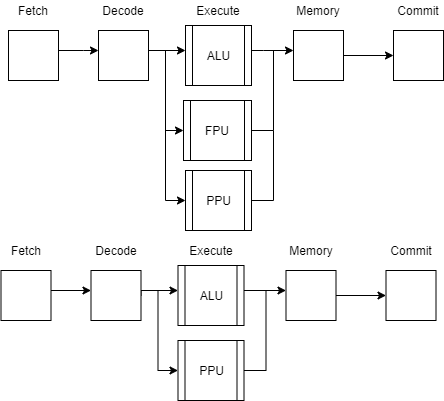
\includegraphics[width=0.5\linewidth]{img/use_cases.png}
    \caption{A visualization of the two possible use cases of the PPU$^{light}$. }
    \label{fig:use_cases}
\end{figure}


We extended the RISC-V ISA to support posit operations keeping in mind the minimalism of RISC-V. The core idea is to implement basic posit operations (addition, multiplication and others) using other wider types as backends. Therefore, we did not introduce new ad-hoc registers for posits. Instead, we aimed to reuse existing floating point and integer registers, providing conversion instructions from/to floating point (on float registers) and fixed point (on integer registers) numbers. 

Note that, unlike floating point numbers, when converting between posit and fixed point, the size of the latter depends on the posit characteristics. From now on we will refer to  a fixed point with $N$ overall bits and $N/2$ bits for the mantissa  as fx$\left<N\right>$. Then, a posit$\left<8,0\right>$ will be converted to fx$\left<16\right>$,  a posit$\left<16,0\right>$ to fx$\left<32\right>$ and a posit$\left<16,1\right>$ to fx$\left<64\right>$.

Since we employ posits with an overall size of 16 or 8 bits, we are performing a \hl{lossy} data compression by a factor of 2 or 4 if we start from an IEEE FP32 format (maintaining a similar \hl{inference} accuracy, in machine learning and neural network tasks, as demonstrated in our previous works \cite{coco_et_al_ieeespm_2020,coco2020sensors}). Moreover, even if we use a wider backend to perform computations, the data expansion is performed only within the posit processing unit. Therefore, we are transferring compressed data from memory to CPU integer/float registers. This means that just by using posits as a \hl{lossy} compressed information storage can reduce the amount of data transferred up to a factor 4.

The instruction encoding uses the suffix \texttt{'b0001011} (6 least significant bits) that is reserved for custom ISA extension.

As listed in Table \ref{tab:rvxposit}, we added the following instructions:
\begin{itemize}
    \item Floating point and posit conversions
    \begin{itemize}
        \item \texttt{FCVT.S.P8/FCVT.P8.S}: \\Float to/from posit$\left<8,0\right>$ conversion
        \item \texttt{FCVT.S.P16.0/FCVT.P16.0.S}:\\ Float to/from posit$\left<16,0\right>$ conversion
        \item \texttt{FCVT.S.P16.1/FCVT.P16.1.S}: \\Float to/from posit$\left<16,1\right>$
    \end{itemize}
    \item Fixed point and posit conversions
    \begin{itemize}
        \item \texttt{FXCVT.H.P8/FXCVT.P8.H}: \\fx$\left<16\right>$ to/from posit$\left<8,0\right>$ conversion
        \item \texttt{FXCVT.W.P16.0/FXCVT.P16.0.W}:\\ fx$\left<32\right>$ to/from posit$\left<16,0\right>$ conversion
        \item \texttt{FXCVT.L.P16.1/FXCVT.P16.1.L}: \\fx$\left<64\right>$ to/from posit$\left<16,1\right>$
    \end{itemize}   
    \item Posit to posit conversions
    \begin{itemize}
        \item \texttt{FCVT.P8.P16.0/FCVT.P16.0.P8}: \\posit$\left<8,0\right>$ to/from posit$\left<16,0\right>$ conversion
        \item \texttt{FCVT.P16.1.P16.0/FCVT.P16.0.P16.1}:\\
        posit$\left<16,1\right>$ to/from posit$\left<16,0\right>$ conversion
        \item \texttt{FCVT.P8.P16.1/FCVT.P16.1.P8}:
        \\posit$\left<16,1\right>$ to/from posit$\left<8,0\right>$ conversion
        \end{itemize}       
\end{itemize}

\begin{table*}
\caption{Instruction listing for RISC-V RVXposit extension}
\begin{small}
\begin{center}
\begin{tabular}{p{0in}p{0.4in}p{0.05in}p{0.05in}p{0.05in}p{0.05in}p{0.4in}p{0.6in}p{0.4in}p{0.6in}p{0.7in}l}
&
\multicolumn{1}{l}{\instbit{31}} &
\multicolumn{1}{r}{\instbit{27}} &
\instbit{26} &
\instbit{25} &
\multicolumn{1}{l}{\instbit{24}} &
\multicolumn{1}{r}{\instbit{20}} &
\instbitrange{19}{15} &
\instbitrange{14}{12} &
\instbitrange{11}{7} &
\instbitrange{6}{0} \\
\cline{2-11}

&
\multicolumn{4}{|c|}{1100000} &
\multicolumn{2}{c|}{00010} &
\multicolumn{1}{c|}{rs1} &
\multicolumn{1}{c|}{000} &
\multicolumn{1}{c|}{rd} &
\multicolumn{1}{c|}{0001011} & FCVT.S.P8 \\
\cline{2-11}


&
\multicolumn{4}{|c|}{1100000} &
\multicolumn{2}{c|}{00011} &
\multicolumn{1}{c|}{rs1} &
\multicolumn{1}{c|}{000} &
\multicolumn{1}{c|}{rd} &
\multicolumn{1}{c|}{0001011} & FCVT.S.P16.0 \\
\cline{2-11}


&
\multicolumn{4}{|c|}{1100000} &
\multicolumn{2}{c|}{00011} &
\multicolumn{1}{c|}{rs1} &
\multicolumn{1}{c|}{010} &
\multicolumn{1}{c|}{rd} &
\multicolumn{1}{c|}{0001011} & FCVT.S.P16.1 \\
\cline{2-11}


&
\multicolumn{4}{|c|}{1101000} &
\multicolumn{2}{c|}{00010} &
\multicolumn{1}{c|}{rs1} &
\multicolumn{1}{c|}{000} &
\multicolumn{1}{c|}{rd} &
\multicolumn{1}{c|}{0001011} & FCVT.P8.S \\
\cline{2-11}


&
\multicolumn{4}{|c|}{1101000} &
\multicolumn{2}{c|}{00011} &
\multicolumn{1}{c|}{rs1} &
\multicolumn{1}{c|}{000} &
\multicolumn{1}{c|}{rd} &
\multicolumn{1}{c|}{0001011} & FCVT.P16.0.S \\
\cline{2-11}


&
\multicolumn{4}{|c|}{1101000} &
\multicolumn{2}{c|}{00011} &
\multicolumn{1}{c|}{rs1} &
\multicolumn{1}{c|}{010} &
\multicolumn{1}{c|}{rd} &
\multicolumn{1}{c|}{0001011} & FCVT.P16.1.S \\
\cline{2-11}


&
\multicolumn{4}{|c|}{1100000} &
\multicolumn{2}{c|}{00010} &
\multicolumn{1}{c|}{rs1} &
\multicolumn{1}{c|}{001} &
\multicolumn{1}{c|}{rd} &
\multicolumn{1}{c|}{0001011} & FXCVT.H.P8 \\
\cline{2-11}


&
\multicolumn{4}{|c|}{1100000} &
\multicolumn{2}{c|}{00011} &
\multicolumn{1}{c|}{rs1} &
\multicolumn{1}{c|}{001} &
\multicolumn{1}{c|}{rd} &
\multicolumn{1}{c|}{0001011} & FXCVT.W.P16.0 \\
\cline{2-11}


&
\multicolumn{4}{|c|}{1100000} &
\multicolumn{2}{c|}{00011} &
\multicolumn{1}{c|}{rs1} &
\multicolumn{1}{c|}{011} &
\multicolumn{1}{c|}{rd} &
\multicolumn{1}{c|}{0001011} & FXCVT.L.P16.1 \\
\cline{2-11}


&
\multicolumn{4}{|c|}{1101000} &
\multicolumn{2}{c|}{00010} &
\multicolumn{1}{c|}{rs1} &
\multicolumn{1}{c|}{001} &
\multicolumn{1}{c|}{rd} &
\multicolumn{1}{c|}{0001011} & FXCVT.P8.H \\
\cline{2-11}


&
\multicolumn{4}{|c|}{1101000} &
\multicolumn{2}{c|}{00011} &
\multicolumn{1}{c|}{rs1} &
\multicolumn{1}{c|}{001} &
\multicolumn{1}{c|}{rd} &
\multicolumn{1}{c|}{0001011} & FXCVT.P16.0.W \\
\cline{2-11}


&
\multicolumn{4}{|c|}{1101000} &
\multicolumn{2}{c|}{00011} &
\multicolumn{1}{c|}{rs1} &
\multicolumn{1}{c|}{011} &
\multicolumn{1}{c|}{rd} &
\multicolumn{1}{c|}{0001011} & FXCVT.P16.1.L \\
\cline{2-11}


&
\multicolumn{4}{|c|}{1101000} &
\multicolumn{2}{c|}{00010} &
\multicolumn{1}{c|}{rs1} &
\multicolumn{1}{c|}{001} &
\multicolumn{1}{c|}{rd} &
\multicolumn{1}{c|}{0001011} & FXCVT.P8.H \\
\cline{2-11}


&
\multicolumn{4}{|c|}{1101000} &
\multicolumn{2}{c|}{00011} &
\multicolumn{1}{c|}{rs1} &
\multicolumn{1}{c|}{001} &
\multicolumn{1}{c|}{rd} &
\multicolumn{1}{c|}{0001011} & FXCVT.P16.0.W \\
\cline{2-11}


&
\multicolumn{4}{|c|}{1101000} &
\multicolumn{2}{c|}{00011} &
\multicolumn{1}{c|}{rs1} &
\multicolumn{1}{c|}{011} &
\multicolumn{1}{c|}{rd} &
\multicolumn{1}{c|}{0001011} & FXCVT.P16.1.L \\
\cline{2-11}


&
\multicolumn{4}{|c|}{1100000} &
\multicolumn{2}{c|}{00010} &
\multicolumn{1}{c|}{rs1} &
\multicolumn{1}{c|}{100} &
\multicolumn{1}{c|}{rd} &
\multicolumn{1}{c|}{0001011} & FCVT.P8.P16.0 \\
\cline{2-11}


&
\multicolumn{4}{|c|}{1100000} &
\multicolumn{2}{c|}{00011} &
\multicolumn{1}{c|}{rs1} &
\multicolumn{1}{c|}{100} &
\multicolumn{1}{c|}{rd} &
\multicolumn{1}{c|}{0001011} & FCVT.P16.0.P8 \\
\cline{2-11}


&
\multicolumn{4}{|c|}{1101000} &
\multicolumn{2}{c|}{00011} &
\multicolumn{1}{c|}{rs1} &
\multicolumn{1}{c|}{111} &
\multicolumn{1}{c|}{rd} &
\multicolumn{1}{c|}{0001011} & FCVT.P16.1.P16.0 \\
\cline{2-11}


&
\multicolumn{4}{|c|}{1101000} &
\multicolumn{2}{c|}{00010} &
\multicolumn{1}{c|}{rs1} &
\multicolumn{1}{c|}{101} &
\multicolumn{1}{c|}{rd} &
\multicolumn{1}{c|}{0001011} & FCVT.P16.1.P8 \\
\cline{2-11}


&
\multicolumn{4}{|c|}{1100000} &
\multicolumn{2}{c|}{00011} &
\multicolumn{1}{c|}{rs1} &
\multicolumn{1}{c|}{110} &
\multicolumn{1}{c|}{rd} &
\multicolumn{1}{c|}{0001011} & FCVT.P8.P16.1 \\
\cline{2-11}


&
\multicolumn{4}{|c|}{1101000} &
\multicolumn{2}{c|}{00011} &
\multicolumn{1}{c|}{rs1} &
\multicolumn{1}{c|}{101} &
\multicolumn{1}{c|}{rd} &
\multicolumn{1}{c|}{0001011} & FCVT.P16.0.P16.1 \\
\cline{2-11}


\end{tabular}
\end{center}
\end{small}
\label{tab:rvxposit}
\end{table*}


Once the instructions have been encoded we need to provide a high-level interface to use them. The idea is to implement a C intrinsic for each instruction exploiting the inline assembly \texttt{\_\_asm\_\_} operator to emit the byte code associated with the specific instruction.
This approach avoids us to implement the code generation inside the compiler. Instead, we let the compiler choose the proper registers for the intrinsic exploiting C/C++ register allocation with the keyword \texttt{register}.

Listing \ref{lst:fcvtin} shows an intrinsic example for the float to posit$\left<8,0\right>$ conversion. The many \texttt{.set} directives are used to set RISC-V register identifiers. The \texttt{.byte} directive is used to emit the four bytes that compose the instruction. Comparing the four bytes of the instruction with the encoding in Table \ref{tab:rvxposit} we can see that both \texttt{rs1} and \texttt{rd} (source and destination register) are not being explicitly set in the intrinsic. Finally, the two register allocations in the function header use the RISC-V standard register names for input and output passing.
\vspace{1em}
\begin{lstlisting}[
  caption=Intrinsic example for FCVT.S.P8,
  label=lst:fcvtin,
]
int __fcvt_f32_p8 (float a) {
 register float p1 asm (``fa0") = a;
 register int result asm (``a1");
 __asm__ volatile(
  ``"
  ``.set rfs0,8\n"
  ``.set rfs1,9\n"
  ...
  ``.set op,0xb\n"
  ``.set opf1,0x0\n"
  ``.set opf2,0x2\n"
  ``.set opf3,0x60\n"
  ``.byte  op|((r%[result]&1) <<7),
          ((r%[result]>>1)&0xF)|(opf1<<4)|((r%1&1)<<7),
          ((opf2&0xF) << 4) | ((r%1>>1)&0xF),
          ((opf2>>4)&0x1)|(opf3<<1)"
  : [result] ``=r"(result)
  :``f"(p1), ``[result]"(result));
 return result;
}
\end{lstlisting}

We instrumented the cppPosit library to be compiled with specific flags to directly use said hardware instructions instead of using software emulation. For example, without hardware support, the conversion between float and posit needs a series of bit manipulations, done in software. If we provide PPU support the same conversion results in a single call to the \texttt{FCVT.S.*/FCVT.*.S} instruction. 

This approach has three key aspects:
\begin{itemize}
    \item We implemented some core posit operations that can not be implemented as $\mathcal{L}1$ operations
    \item We discarded other slow instructions that require activation and withdrawal like in an external execution unit.
    \item We may seamlessly run in a super-scalar environment with multiple parallel execution units since we only used native integer and floating point registers.
\end{itemize}



To provide a circuit design for our PPU$^{light}$ we considered several key points to simplify the final logic design:
\begin{itemize}
    \item IEEE floating point values are encoded in a module and sign-like representation while posits are encoded using 2's complement representation. Therefore, when converting from IEEE floats we just ignore the sign and build the positive posit. Then we use the sign to apply the 2's complement to the result if negative.
    \item Given a Posit$\left<16,0\right>$ the size of the regime spans from a minimum of 2 to a maximum of 15 bits. As a result, the mantissa size spans from a minimum of 0 to a maximum of 12 bits. This means that, given a 23-bit mantissa IEEE Float, the 8 least significant bits of the float are set to 0. A similar reasoning holds for Posit$\left<8,0\right>$. 
    \item We can build the Posit$\left<X,0\right>$ regime arithmetically shifting an appropriate value by the $\log_2{X}$ least significant bits of the FP32 normalized exponent. For Posit$\left<16,0\right>$ we shift the signed integer represented by $2^{15}$ (\texttt{8000} in hexadecimal notation, as in Figure \ref{fig:fp_exp_reg_encoder}). For Posit$\left<8,0\right>$, we shift the signed integer represented by $2^{7}$. Furthermore, we always build the regime starting from the absolute value of the normalized FP32 exponent. It can be then transformed to the ``negative" regime in case of negative exponent values as in Figure \ref{fig:fp_exp_reg_encoder}. In this circuit, we take the floating point exponent on 8 bits and produce the regime bits corresponding to that exponent. To generate the regime, we arithmetically shift the signed integer represented by $2^{15}$ (\texttt{'h8000}) by the amount specified by the 4 least significant digits of the floating point exponent. The same procedure holds for both negative and positive exponents, with just a negation at the end to restore the correct sign. 
    \item Decoding the regime is particularly interesting since we need to employ a \emph{find first set} module (or \emph{find first unset}) to evaluate the regime length. The output of the \emph{find first set} module is the index $i$ of the highest set bit (discarding the sign if present). Therefore, as reported in Figure \ref{fig:fp_exp_reg_decoder}, the regime length is actually computed as $l=14-i$. In the end, the $k$-value (which is the non-normalized floating point exponent) is obtained from the regime length as $-l$ or $l+1$, depending on the regime ``sign''. In the circuit of Figure \ref{fig:fp_exp_reg_decoder}, we take the regime field and output the corresponding value of $k$. The core part is represented by the two \textit{find high} modules that help to compute the number of subsequent bit set (or unset). If we subtract this number at the maximum length of the regime (that is $14$, or \texttt{'he} in hexadecimal notation) we get the actual regime length $l$. Finally, if we follow we can retrieve $k$ from $l$.  
\end{itemize}

\begin{figure}
    \centering
    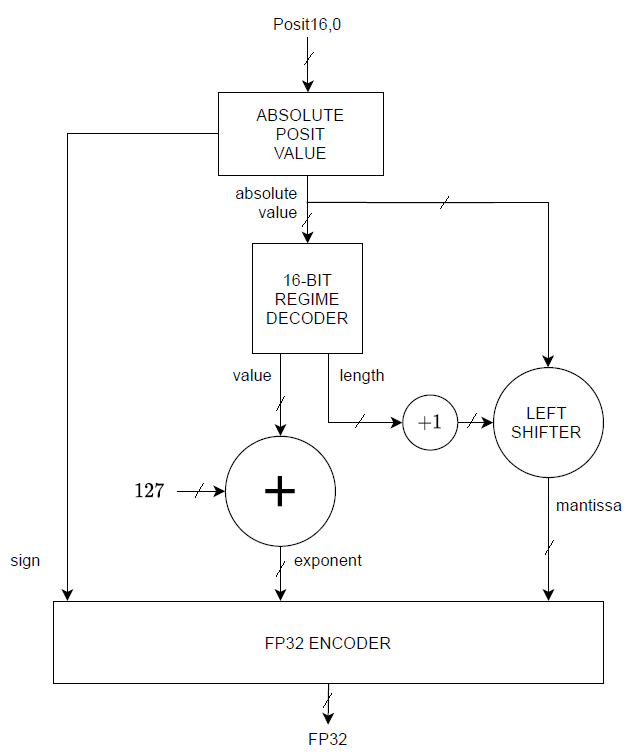
\includegraphics[width=0.5\linewidth]{img/p16_fp32.PNG}
    \caption{Logical circuit for the posit$\left<16,0\right>$ to 32-bit floating point converter.}
    \label{fig:p16_fp32_circ}
\end{figure}

\begin{figure}
    \centering
    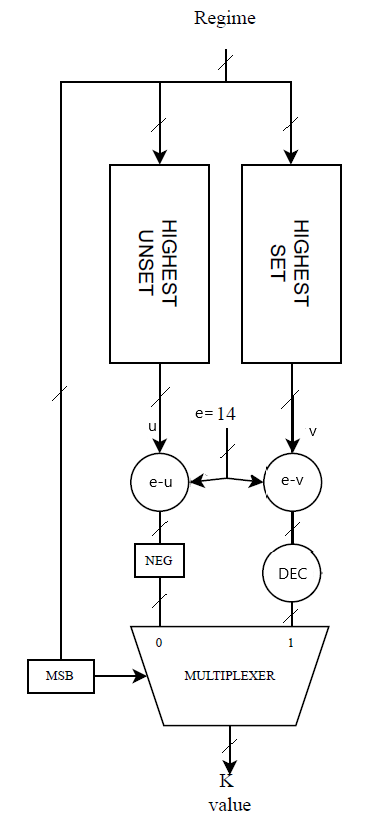
\includegraphics[width=0.56\linewidth]{img/regime_decoder.PNG}
    \caption{Logical circuit for the posit$\left<16,0\right>$ regime \textbf{decoder}}
    \label{fig:fp_exp_reg_decoder}
\end{figure}


In Figure \ref{fig:p16_fp32_circ}, we show \hl{a simplified} circuit for conversion from posit$\left<16,0\right>$ to FP32. The 16-bit regime decoder module is implemented by \hl{the simplified} circuit shown in Figure \ref{fig:fp_exp_reg_decoder}. Note how when converting to IEEE floats we firstly compute the absolute value of the posit number and then convert it to a floating point one. At the end of the circuit, we just replicate the bit sign of the posit in the bit sign of the floating point, being represented in the sign and module. 


In Figure \ref{fig:fp32_p16_circ}, we show \hl{a simplified} circuit for conversion from FP32 to posit$\left<16,0\right>$. The first multiplexer in the cascade of two multiplexers takes the exponent value as input; this input acts as a mask to detect \textit{Not A Real (NaR)} values. The 16-bit regime encoder module is implemented by \hl{the simplified} circuit shown in Figure \ref{fig:fp_exp_reg_encoder}. Note how when converting from IEEE floats we just ignore the sign and build the positive posit and then we use the sign to apply the 2's complement to the result if negative. Furthermore, we build the different posit fields considering their maximum possible length without computing any length but the regime one, making the circuit simpler.

\begin{figure}
    \centering
    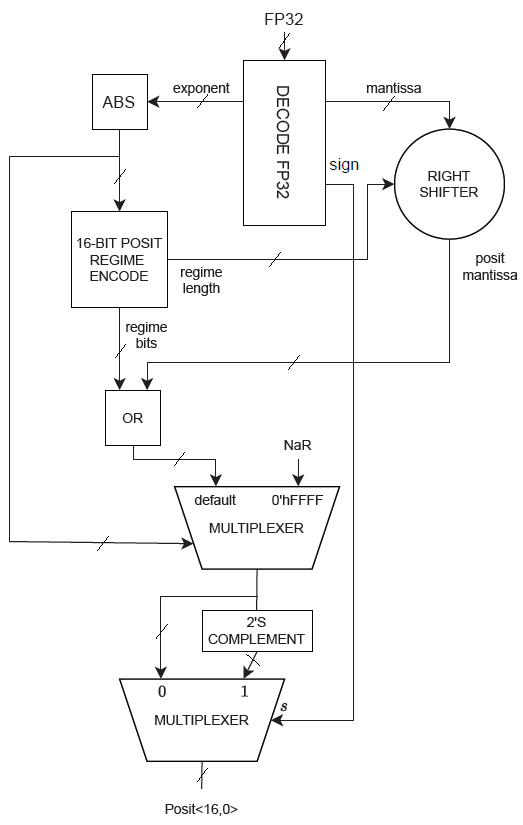
\includegraphics[width=0.5\linewidth]{img/fp32_p16.PNG}
    \caption{Logical circuit for the 32-bit floating point to posit$\left<16,0\right>$ converter. \textit{NaR} is \textit{Not A Real}.}
    \label{fig:fp32_p16_circ}
\end{figure}

\begin{figure}
    \centering
    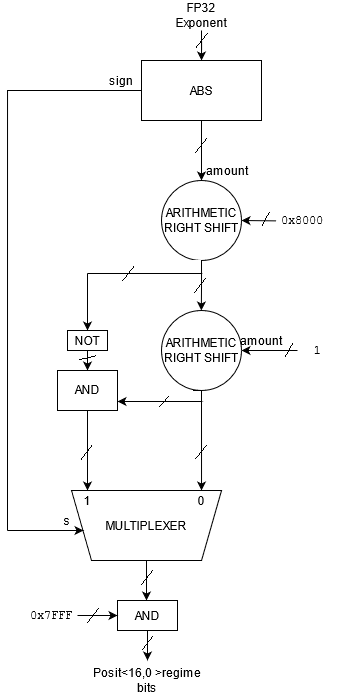
\includegraphics[width=0.5\linewidth]{img/regime_encoder.png}
    \caption{Logical circuit for the posit$\left<16,0\right>$ regime \textbf{encoder}. \textit{Amount} is the number of positions to shift the other input in the \textit{Arithmetic Right Shift} module.}
    \label{fig:fp_exp_reg_encoder}
\end{figure}



%\section{Enabling fast arithmetic operations for reals without decoding}
% Insert further chapters using the following syntax
% \input{Source_Folder_Name/FileName}


\cleardoublepage
\phantomsection
\addcontentsline{toc}{chapter}{\bibname}
\small
\bibliographystyle{plain}
\bibliography{thesis}

\end{document}
